\documentclass[11pt]{article}

% The four macros of the header standard; tools/zenodo/publish_revision.py patches them when it reserves the DOI.
\newcommand{\doctype}{Preprint}
\newcommand{\docversion}{v1.00.000}
\newcommand{\docdate}{8 November 2026}
\newcommand{\versiondoi}{10.5281/zenodo.24053188}
\newcommand{\conceptdoi}{10.5281/zenodo.24053187}
\newcommand{\docidentity}{CAOS\_Contraste, the validation of the risk models of a bank}

% The packages and conventions every Contraste manuscript shares (CAOS_MANAGE conventions/manuscript-content-bar.md
% section 2). A document sets its class, the four header macros and \docidentity, then % The packages and conventions every Contraste manuscript shares (CAOS_MANAGE conventions/manuscript-content-bar.md
% section 2). A document sets its class, the four header macros and \docidentity, then % The packages and conventions every Contraste manuscript shares (CAOS_MANAGE conventions/manuscript-content-bar.md
% section 2). A document sets its class, the four header macros and \docidentity, then \input{../_shared/preamble}.
\usepackage[T1]{fontenc}
\usepackage[utf8]{inputenc}
\usepackage{lmodern}
\usepackage{microtype}
\usepackage[a4paper,margin=2.5cm]{geometry}
\usepackage{amsmath,amssymb,amsthm,mathtools,bm}
\usepackage{graphicx}
\usepackage{booktabs,longtable,tabularx,array,multirow}
\usepackage{siunitx}
\usepackage{algorithm}
\usepackage{algpseudocode}
\usepackage{caption,subcaption}
\usepackage{xcolor}
\usepackage[numbers,sort&compress]{natbib}
\usepackage[hidelinks]{hyperref}
\usepackage{cleveref}
\usepackage{orcidlink}

\sisetup{group-separator={,},group-minimum-digits=4,detect-all}
\graphicspath{{figures/}{../figures/}}
\captionsetup{font=small,labelfont=bf}
\setlength{\LTcapwidth}{\textwidth}

% Theorem environments for the Theory sections of the manuscripts.
\newtheorem{proposition}{Proposition}
\newtheorem{lemma}{Lemma}
\newtheorem{corollary}{Corollary}
\theoremstyle{definition}
\newtheorem{definition}{Definition}
\newtheorem{assumption}{Assumption}
\theoremstyle{remark}
\newtheorem{remark}{Remark}

% Notation shared by the documents (each defines it again in its notation table).
\newcommand{\E}{\mathbb{E}}
\newcommand{\Prob}{\mathbb{P}}
\newcommand{\Var}{\operatorname{Var}}
\newcommand{\Cov}{\operatorname{Cov}}
\newcommand{\VaR}{\operatorname{VaR}}
\newcommand{\ES}{\operatorname{ES}}
\newcommand{\PD}{\mathrm{PD}}
\newcommand{\LGD}{\mathrm{LGD}}
\newcommand{\EAD}{\mathrm{EAD}}
\newcommand{\ECL}{\mathrm{ECL}}
\newcommand{\indic}{\mathbf{1}}
\newcommand{\R}{\mathbb{R}}
\newcommand{\dd}{\,\mathrm{d}}

% The page-1 header block (CAOS_MANAGE conventions/manuscript-header-standard.md). The document defines \doctype,
% \docversion, \docdate, \versiondoi, \conceptdoi and \docidentity before this file; the publishing tool patches the four
% macros of the standard when it reserves the version DOI.
\newcommand{\docrepo}{github.com/fsantibanezleal/CAOS\_Contraste}
\newcommand{\headerblock}{%
\begin{center}
\fbox{\parbox{0.94\textwidth}{\small\raggedright
\textbf{\doctype} \quad$\cdot$\quad \docversion, \docdate \quad$\cdot$\quad Licence CC BY 4.0\\[2pt]
CAOS open-research programme \quad$\cdot$\quad \docidentity\\[2pt]
Version DOI \href{https://doi.org/\versiondoi}{\texttt{\versiondoi}} \quad$\cdot$\quad
concept DOI (always latest) \href{https://doi.org/\conceptdoi}{\texttt{\conceptdoi}}\\[2pt]
Not peer reviewed. Source code, data and computational records: \href{https://\docrepo}{\texttt{\docrepo}}
}}
\end{center}
\vspace{4pt}}
.
\usepackage[T1]{fontenc}
\usepackage[utf8]{inputenc}
\usepackage{lmodern}
\usepackage{microtype}
\usepackage[a4paper,margin=2.5cm]{geometry}
\usepackage{amsmath,amssymb,amsthm,mathtools,bm}
\usepackage{graphicx}
\usepackage{booktabs,longtable,tabularx,array,multirow}
\usepackage{siunitx}
\usepackage{algorithm}
\usepackage{algpseudocode}
\usepackage{caption,subcaption}
\usepackage{xcolor}
\usepackage[numbers,sort&compress]{natbib}
\usepackage[hidelinks]{hyperref}
\usepackage{cleveref}
\usepackage{orcidlink}

\sisetup{group-separator={,},group-minimum-digits=4,detect-all}
\graphicspath{{figures/}{../figures/}}
\captionsetup{font=small,labelfont=bf}
\setlength{\LTcapwidth}{\textwidth}

% Theorem environments for the Theory sections of the manuscripts.
\newtheorem{proposition}{Proposition}
\newtheorem{lemma}{Lemma}
\newtheorem{corollary}{Corollary}
\theoremstyle{definition}
\newtheorem{definition}{Definition}
\newtheorem{assumption}{Assumption}
\theoremstyle{remark}
\newtheorem{remark}{Remark}

% Notation shared by the documents (each defines it again in its notation table).
\newcommand{\E}{\mathbb{E}}
\newcommand{\Prob}{\mathbb{P}}
\newcommand{\Var}{\operatorname{Var}}
\newcommand{\Cov}{\operatorname{Cov}}
\newcommand{\VaR}{\operatorname{VaR}}
\newcommand{\ES}{\operatorname{ES}}
\newcommand{\PD}{\mathrm{PD}}
\newcommand{\LGD}{\mathrm{LGD}}
\newcommand{\EAD}{\mathrm{EAD}}
\newcommand{\ECL}{\mathrm{ECL}}
\newcommand{\indic}{\mathbf{1}}
\newcommand{\R}{\mathbb{R}}
\newcommand{\dd}{\,\mathrm{d}}

% The page-1 header block (CAOS_MANAGE conventions/manuscript-header-standard.md). The document defines \doctype,
% \docversion, \docdate, \versiondoi, \conceptdoi and \docidentity before this file; the publishing tool patches the four
% macros of the standard when it reserves the version DOI.
\newcommand{\docrepo}{github.com/fsantibanezleal/CAOS\_Contraste}
\newcommand{\headerblock}{%
\begin{center}
\fbox{\parbox{0.94\textwidth}{\small\raggedright
\textbf{\doctype} \quad$\cdot$\quad \docversion, \docdate \quad$\cdot$\quad Licence CC BY 4.0\\[2pt]
CAOS open-research programme \quad$\cdot$\quad \docidentity\\[2pt]
Version DOI \href{https://doi.org/\versiondoi}{\texttt{\versiondoi}} \quad$\cdot$\quad
concept DOI (always latest) \href{https://doi.org/\conceptdoi}{\texttt{\conceptdoi}}\\[2pt]
Not peer reviewed. Source code, data and computational records: \href{https://\docrepo}{\texttt{\docrepo}}
}}
\end{center}
\vspace{4pt}}
.
\usepackage[T1]{fontenc}
\usepackage[utf8]{inputenc}
\usepackage{lmodern}
\usepackage{microtype}
\usepackage[a4paper,margin=2.5cm]{geometry}
\usepackage{amsmath,amssymb,amsthm,mathtools,bm}
\usepackage{graphicx}
\usepackage{booktabs,longtable,tabularx,array,multirow}
\usepackage{siunitx}
\usepackage{algorithm}
\usepackage{algpseudocode}
\usepackage{caption,subcaption}
\usepackage{xcolor}
\usepackage[numbers,sort&compress]{natbib}
\usepackage[hidelinks]{hyperref}
\usepackage{cleveref}
\usepackage{orcidlink}

\sisetup{group-separator={,},group-minimum-digits=4,detect-all}
\graphicspath{{figures/}{../figures/}}
\captionsetup{font=small,labelfont=bf}
\setlength{\LTcapwidth}{\textwidth}

% Theorem environments for the Theory sections of the manuscripts.
\newtheorem{proposition}{Proposition}
\newtheorem{lemma}{Lemma}
\newtheorem{corollary}{Corollary}
\theoremstyle{definition}
\newtheorem{definition}{Definition}
\newtheorem{assumption}{Assumption}
\theoremstyle{remark}
\newtheorem{remark}{Remark}

% Notation shared by the documents (each defines it again in its notation table).
\newcommand{\E}{\mathbb{E}}
\newcommand{\Prob}{\mathbb{P}}
\newcommand{\Var}{\operatorname{Var}}
\newcommand{\Cov}{\operatorname{Cov}}
\newcommand{\VaR}{\operatorname{VaR}}
\newcommand{\ES}{\operatorname{ES}}
\newcommand{\PD}{\mathrm{PD}}
\newcommand{\LGD}{\mathrm{LGD}}
\newcommand{\EAD}{\mathrm{EAD}}
\newcommand{\ECL}{\mathrm{ECL}}
\newcommand{\indic}{\mathbf{1}}
\newcommand{\R}{\mathbb{R}}
\newcommand{\dd}{\,\mathrm{d}}

% The page-1 header block (CAOS_MANAGE conventions/manuscript-header-standard.md). The document defines \doctype,
% \docversion, \docdate, \versiondoi, \conceptdoi and \docidentity before this file; the publishing tool patches the four
% macros of the standard when it reserves the version DOI.
\newcommand{\docrepo}{github.com/fsantibanezleal/CAOS\_Contraste}
\newcommand{\headerblock}{%
\begin{center}
\fbox{\parbox{0.94\textwidth}{\small\raggedright
\textbf{\doctype} \quad$\cdot$\quad \docversion, \docdate \quad$\cdot$\quad Licence CC BY 4.0\\[2pt]
CAOS open-research programme \quad$\cdot$\quad \docidentity\\[2pt]
Version DOI \href{https://doi.org/\versiondoi}{\texttt{\versiondoi}} \quad$\cdot$\quad
concept DOI (always latest) \href{https://doi.org/\conceptdoi}{\texttt{\conceptdoi}}\\[2pt]
Not peer reviewed. Source code, data and computational records: \href{https://\docrepo}{\texttt{\docrepo}}
}}
\end{center}
\vspace{4pt}}

% Every number the prose quotes is a macro written by make_numbers.py from the experiment results and the committed documents.
% Generated by make_numbers.py from experiments/results and data/derived: do not edit.
\newcommand{\CmBaseBB}{0.523}
\newcommand{\CmBaseBin}{0.313}
\newcommand{\CmBaseCov}{0.8946}
\newcommand{\CmBaseLight}{green}
\newcommand{\CmBaseM}{3,151}
\newcommand{\CmFairAboveTen}{6}
\newcommand{\CmFairAmber}{4}
\newcommand{\CmFairGreen}{2}
\newcommand{\CmFairGreenHi}{0.1992}
\newcommand{\CmFairGreenLo}{0.1871}
\newcommand{\CmFairGreenOverNull}{3.4}
\newcommand{\CmFairMax}{0.2629}
\newcommand{\CmFairMin}{0.1871}
\newcommand{\CmFairPairs}{6}
\newcommand{\CmFairQMax}{8,113}
\newcommand{\CmFairQMin}{4,485}
\newcommand{\CmHalfBB}{$4.56 \times 10^{-52}$}
\newcommand{\CmHalfBin}{$1.19 \times 10^{-194}$}
\newcommand{\CmHalfCov}{0.7099}
\newcommand{\CmHalfLight}{red}
\newcommand{\CmHalfM}{3,151}
\newcommand{\CmNcal}{1,471}
\newcommand{\CmOneBB}{0.037}
\newcommand{\CmOneBin}{$2.58 \times 10^{-4}$}
\newcommand{\CmOneCov}{0.8800}
\newcommand{\CmOneLight}{amber}
\newcommand{\CmOneM}{3,151}
\newcommand{\CmPoolBB}{$2.86 \times 10^{-20}$}
\newcommand{\CmPoolBin}{$2.16 \times 10^{-207}$}
\newcommand{\CmPoolCov}{0.8089}
\newcommand{\CmPoolLight}{red}
\newcommand{\CmPoolM}{12,604}
\newcommand{\CmQuarterBB}{$2.13 \times 10^{-35}$}
\newcommand{\CmQuarterBin}{$3.69 \times 10^{-127}$}
\newcommand{\CmQuarterCov}{0.7509}
\newcommand{\CmQuarterLight}{red}
\newcommand{\CmQuarterM}{3,151}
\newcommand{\CmRecomputeDiff}{$1.0 \times 10^{-16}$}
\newcommand{\CmResDraws}{199}
\newcommand{\CmResDrop}{0.0857}
\newcommand{\CmResN}{316}
\newcommand{\CmResNullMean}{0.0007}
\newcommand{\CmResNullP}{0.0243}
\newcommand{\CmResP}{0.005}
\newcommand{\CovBBMaxExact}{0.0499}
\newcommand{\CovBBMaxRate}{0.054}
\newcommand{\CovBBOverBound}{0}
\newcommand{\CovEngineMismatches}{0}
\newcommand{\CovExBBA}{0.047}
\newcommand{\CovExBBB}{0.048}
\newcommand{\CovExBBC}{0.050}
\newcommand{\CovExBBMaxTenth}{0.046}
\newcommand{\CovExBBMinTenth}{0.015}
\newcommand{\CovExBinA}{0.059}
\newcommand{\CovExBinB}{0.162}
\newcommand{\CovExBinC}{0.376}
\newcommand{\CovExBinMaxEight}{0.512}
\newcommand{\CovExBinMaxFour}{0.379}
\newcommand{\CovExBinMaxOne}{0.161}
\newcommand{\CovExBinMaxTenth}{0.055}
\newcommand{\CovExBinMinEight}{0.506}
\newcommand{\CovExBinMinFour}{0.370}
\newcommand{\CovExBinMinOne}{0.150}
\newcommand{\CovExBinMinTenth}{0.050}
\newcommand{\CovGridCells}{21}
\newcommand{\CovMcCompare}{46}
\newcommand{\CovMcExactMaxZ}{2.0}
\newcommand{\CovMeanAFive}{0.895}
\newcommand{\CovMeanATen}{0.891}
\newcommand{\CovMeanATwenty}{0.881}
\newcommand{\CovMeanATwo}{0.898}
\newcommand{\CovMeanBFive}{0.896}
\newcommand{\CovMeanBTen}{0.890}
\newcommand{\CovMeanBTwenty}{0.881}
\newcommand{\CovMeanBTwo}{0.898}
\newcommand{\CovMeanCFive}{0.895}
\newcommand{\CovMeanCTen}{0.891}
\newcommand{\CovMeanCTwenty}{0.882}
\newcommand{\CovMeanCTwo}{0.898}
\newcommand{\CovNormalBinA}{0.062}
\newcommand{\CovNormalBinB}{0.166}
\newcommand{\CovNormalBinC}{0.380}
\newcommand{\CovNormalMaxErr}{0.030}
\newcommand{\CovOracleCutA}{0.0368}
\newcommand{\CovOracleCutB}{0.0052}
\newcommand{\CovOracleCutC}{$1.2 \times 10^{-5}$}
\newcommand{\CovPowBBAFive}{0.103}
\newcommand{\CovPowBBATen}{0.248}
\newcommand{\CovPowBBATwenty}{0.731}
\newcommand{\CovPowBBATwo}{0.052}
\newcommand{\CovPowBBBFive}{0.076}
\newcommand{\CovPowBBBTen}{0.190}
\newcommand{\CovPowBBBTwenty}{0.489}
\newcommand{\CovPowBBBTwo}{0.053}
\newcommand{\CovPowBBCFive}{0.079}
\newcommand{\CovPowBBCTen}{0.162}
\newcommand{\CovPowBBCTwenty}{0.414}
\newcommand{\CovPowBBCTwo}{0.050}
\newcommand{\CovPowBinAFive}{0.129}
\newcommand{\CovPowBinATen}{0.292}
\newcommand{\CovPowBinATwenty}{0.772}
\newcommand{\CovPowBinATwo}{0.066}
\newcommand{\CovPowBinBFive}{0.204}
\newcommand{\CovPowBinBTen}{0.372}
\newcommand{\CovPowBinBTwenty}{0.686}
\newcommand{\CovPowBinBTwo}{0.173}
\newcommand{\CovPowBinCFive}{0.412}
\newcommand{\CovPowBinCTen}{0.532}
\newcommand{\CovPowBinCTwenty}{0.769}
\newcommand{\CovPowBinCTwo}{0.389}
\newcommand{\CovPowDoubleAFive}{0.114}
\newcommand{\CovPowDoubleATen}{0.273}
\newcommand{\CovPowDoubleATwenty}{0.752}
\newcommand{\CovPowDoubleBFive}{0.122}
\newcommand{\CovPowDoubleBTen}{0.264}
\newcommand{\CovPowDoubleBTwenty}{0.574}
\newcommand{\CovPowDoubleCFive}{0.164}
\newcommand{\CovPowDoubleCTen}{0.286}
\newcommand{\CovPowDoubleCTwenty}{0.565}
\newcommand{\CovPowEqAFive}{0.103}
\newcommand{\CovPowEqATen}{0.248}
\newcommand{\CovPowEqATwenty}{0.731}
\newcommand{\CovPowEqBFive}{0.069}
\newcommand{\CovPowEqBTen}{0.179}
\newcommand{\CovPowEqBTwenty}{0.469}
\newcommand{\CovPowEqCFive}{0.070}
\newcommand{\CovPowEqCTen}{0.146}
\newcommand{\CovPowEqCTwenty}{0.389}
\newcommand{\CovPowHalfAFive}{0.091}
\newcommand{\CovPowHalfATen}{0.224}
\newcommand{\CovPowHalfATwenty}{0.709}
\newcommand{\CovPowHalfBFive}{0.033}
\newcommand{\CovPowHalfBTen}{0.102}
\newcommand{\CovPowHalfBTwenty}{0.341}
\newcommand{\CovPowHalfCFive}{0.020}
\newcommand{\CovPowHalfCTen}{0.055}
\newcommand{\CovPowHalfCTwenty}{0.211}
\newcommand{\CovPowOracleAFive}{0.103}
\newcommand{\CovPowOracleATen}{0.248}
\newcommand{\CovPowOracleATwenty}{0.731}
\newcommand{\CovPowOracleBFive}{0.069}
\newcommand{\CovPowOracleBTen}{0.179}
\newcommand{\CovPowOracleBTwenty}{0.469}
\newcommand{\CovPowOracleCFive}{0.072}
\newcommand{\CovPowOracleCTen}{0.151}
\newcommand{\CovPowOracleCTwenty}{0.399}
\newcommand{\CovPowSeBBAFive}{0.005}
\newcommand{\CovPowSeBBATen}{0.007}
\newcommand{\CovPowSeBBATwenty}{0.007}
\newcommand{\CovPowSeBBATwo}{0.004}
\newcommand{\CovPowSeBBBFive}{0.004}
\newcommand{\CovPowSeBBBTen}{0.006}
\newcommand{\CovPowSeBBBTwenty}{0.008}
\newcommand{\CovPowSeBBBTwo}{0.004}
\newcommand{\CovPowSeBBCFive}{0.004}
\newcommand{\CovPowSeBBCTen}{0.006}
\newcommand{\CovPowSeBBCTwenty}{0.008}
\newcommand{\CovPowSeBBCTwo}{0.003}
\newcommand{\CovPowSeBinAFive}{0.005}
\newcommand{\CovPowSeBinATen}{0.007}
\newcommand{\CovPowSeBinATwenty}{0.007}
\newcommand{\CovPowSeBinATwo}{0.004}
\newcommand{\CovPowSeBinBFive}{0.006}
\newcommand{\CovPowSeBinBTen}{0.008}
\newcommand{\CovPowSeBinBTwenty}{0.007}
\newcommand{\CovPowSeBinBTwo}{0.006}
\newcommand{\CovPowSeBinCFive}{0.008}
\newcommand{\CovPowSeBinCTen}{0.008}
\newcommand{\CovPowSeBinCTwenty}{0.007}
\newcommand{\CovPowSeBinCTwo}{0.008}
\newcommand{\CovPowSeDoubleAFive}{0.005}
\newcommand{\CovPowSeDoubleATen}{0.007}
\newcommand{\CovPowSeDoubleATwenty}{0.007}
\newcommand{\CovPowSeDoubleBFive}{0.005}
\newcommand{\CovPowSeDoubleBTen}{0.007}
\newcommand{\CovPowSeDoubleBTwenty}{0.008}
\newcommand{\CovPowSeDoubleCFive}{0.006}
\newcommand{\CovPowSeDoubleCTen}{0.007}
\newcommand{\CovPowSeDoubleCTwenty}{0.008}
\newcommand{\CovPowSeEqAFive}{0.005}
\newcommand{\CovPowSeEqATen}{0.007}
\newcommand{\CovPowSeEqATwenty}{0.007}
\newcommand{\CovPowSeEqBFive}{0.004}
\newcommand{\CovPowSeEqBTen}{0.006}
\newcommand{\CovPowSeEqBTwenty}{0.008}
\newcommand{\CovPowSeEqCFive}{0.004}
\newcommand{\CovPowSeEqCTen}{0.006}
\newcommand{\CovPowSeEqCTwenty}{0.008}
\newcommand{\CovPowSeHalfAFive}{0.005}
\newcommand{\CovPowSeHalfATen}{0.007}
\newcommand{\CovPowSeHalfATwenty}{0.007}
\newcommand{\CovPowSeHalfBFive}{0.003}
\newcommand{\CovPowSeHalfBTen}{0.005}
\newcommand{\CovPowSeHalfBTwenty}{0.007}
\newcommand{\CovPowSeHalfCFive}{0.002}
\newcommand{\CovPowSeHalfCTen}{0.004}
\newcommand{\CovPowSeHalfCTwenty}{0.006}
\newcommand{\CovPowSeOracleAFive}{0.005}
\newcommand{\CovPowSeOracleATen}{0.007}
\newcommand{\CovPowSeOracleATwenty}{0.007}
\newcommand{\CovPowSeOracleBFive}{0.004}
\newcommand{\CovPowSeOracleBTen}{0.006}
\newcommand{\CovPowSeOracleBTwenty}{0.008}
\newcommand{\CovPowSeOracleCFive}{0.004}
\newcommand{\CovPowSeOracleCTen}{0.006}
\newcommand{\CovPowSeOracleCTwenty}{0.008}
\newcommand{\CovPowSeZinfAFive}{0.005}
\newcommand{\CovPowSeZinfATen}{0.007}
\newcommand{\CovPowSeZinfATwenty}{0.007}
\newcommand{\CovPowSeZinfBFive}{0.004}
\newcommand{\CovPowSeZinfBTen}{0.006}
\newcommand{\CovPowSeZinfBTwenty}{0.008}
\newcommand{\CovPowSeZinfCFive}{0.004}
\newcommand{\CovPowSeZinfCTen}{0.006}
\newcommand{\CovPowSeZinfCTwenty}{0.008}
\newcommand{\CovPowZinfAFive}{0.113}
\newcommand{\CovPowZinfATen}{0.273}
\newcommand{\CovPowZinfATwenty}{0.752}
\newcommand{\CovPowZinfBFive}{0.076}
\newcommand{\CovPowZinfBTen}{0.190}
\newcommand{\CovPowZinfBTwenty}{0.489}
\newcommand{\CovPowZinfCFive}{0.079}
\newcommand{\CovPowZinfCTen}{0.162}
\newcommand{\CovPowZinfCTwenty}{0.414}
\newcommand{\CovReps}{4,000}
\newcommand{\CovSeBBA}{0.003}
\newcommand{\CovSeBBB}{0.003}
\newcommand{\CovSeBBC}{0.003}
\newcommand{\CovSeBinA}{0.004}
\newcommand{\CovSeBinB}{0.006}
\newcommand{\CovSeBinC}{0.008}
\newcommand{\CovSeDoubleA}{0.004}
\newcommand{\CovSeDoubleB}{0.005}
\newcommand{\CovSeDoubleC}{0.005}
\newcommand{\CovSeEqA}{0.003}
\newcommand{\CovSeEqB}{0.004}
\newcommand{\CovSeEqC}{0.003}
\newcommand{\CovSeHalfA}{0.003}
\newcommand{\CovSeHalfB}{0.002}
\newcommand{\CovSeHalfC}{0.001}
\newcommand{\CovSeOracleA}{0.003}
\newcommand{\CovSeOracleB}{0.004}
\newcommand{\CovSeOracleC}{0.003}
\newcommand{\CovSeZinfA}{0.003}
\newcommand{\CovSeZinfB}{0.003}
\newcommand{\CovSeZinfC}{0.003}
\newcommand{\CovSimBinMaxFour}{0.378}
\newcommand{\CovSimBinMaxOne}{0.162}
\newcommand{\CovSimBinMinFour}{0.361}
\newcommand{\CovSimBinMinOne}{0.148}
\newcommand{\CovSinBBA}{0.045}
\newcommand{\CovSinBBB}{0.051}
\newcommand{\CovSinBBC}{0.048}
\newcommand{\CovSinBinA}{0.057}
\newcommand{\CovSinBinB}{0.157}
\newcommand{\CovSinBinC}{0.361}
\newcommand{\CovSinDoubleA}{0.053}
\newcommand{\CovSinDoubleB}{0.089}
\newcommand{\CovSinDoubleC}{0.124}
\newcommand{\CovSinEqA}{0.045}
\newcommand{\CovSinEqB}{0.052}
\newcommand{\CovSinEqC}{0.046}
\newcommand{\CovSinHalfA}{0.040}
\newcommand{\CovSinHalfB}{0.018}
\newcommand{\CovSinHalfC}{0.007}
\newcommand{\CovSinOracleA}{0.045}
\newcommand{\CovSinOracleB}{0.052}
\newcommand{\CovSinOracleC}{0.048}
\newcommand{\CovSinZinfA}{0.049}
\newcommand{\CovSinZinfB}{0.051}
\newcommand{\CovSinZinfC}{0.047}
\newcommand{\CovTotalCells}{35}
\newcommand{\CovTotalReps}{140,000}
\newcommand{\EngSiSeTwenty}{0.0031}
\newcommand{\EngSiSizeTen}{0.194}
\newcommand{\EngSiSizeTwenty}{0.0395}
\newcommand{\EnvEngine}{1.1.0}
\newcommand{\EnvNumpy}{2.4.6}
\newcommand{\EnvScipy}{1.18.1}
\newcommand{\ExPowBBBTen}{0.177}
\newcommand{\ExPowBBCTen}{0.158}
\newcommand{\ExPowBinBTen}{0.354}
\newcommand{\ExPowBinCTen}{0.533}
\newcommand{\ExPowGapCells}{48}
\newcommand{\ExPowGapMax}{0.019}
\newcommand{\ExPowNodes}{2,000}
\newcommand{\ExPowOracleBTen}{0.166}
\newcommand{\ExPowOracleCTen}{0.149}
\newcommand{\ExPowPairs}{3}
\newcommand{\ExPowShapes}{16}
\newcommand{\GranAllowedFull}{8}
\newcommand{\GranAllowedNineteen}{-1}
\newcommand{\GranAllowedNinetyNine}{3}
\newcommand{\GranAllowedThirtyNine}{0}
\newcommand{\GranExactFull}{0.045}
\newcommand{\GranExactNineteen}{0.000}
\newcommand{\GranExactNinetyNine}{0.040}
\newcommand{\GranExactThirtyNine}{0.025}
\newcommand{\GranSmallestFull}{0.005}
\newcommand{\GranSmallestNineteen}{0.050}
\newcommand{\GranSmallestNinetyNine}{0.010}
\newcommand{\GranSmallestThirtyNine}{0.025}
\newcommand{\HypHeld}{7}
\newcommand{\HypPartial}{0}
\newcommand{\HypRefuted}{3}
\newcommand{\HypTotal}{10}
\newcommand{\LimBinEight}{0.514}
\newcommand{\LimBinFour}{0.381}
\newcommand{\LimBinOne}{0.166}
\newcommand{\LimBinTenth}{0.062}
\newcommand{\NbBBFour}{0.0427}
\newcommand{\NbBBOne}{0.0440}
\newcommand{\NbBBTenth}{0.0460}
\newcommand{\NbBinFour}{0.3893}
\newcommand{\NbBinOne}{0.1587}
\newcommand{\NbBinTenth}{0.0600}
\newcommand{\NbCovReps}{1,500}
\newcommand{\NbFixedFiveT}{0.8500}
\newcommand{\NbFixedFiveZ}{0.2000}
\newcommand{\NbFixedTenT}{0.6667}
\newcommand{\NbFixedTenZ}{0.0833}
\newcommand{\NbPermT}{0.5000}
\newcommand{\NbPermZ}{0.0667}
\newcommand{\NbShiftReps}{60}
\newcommand{\NbSitCutTenZ}{0.0850}
\newcommand{\NbSitCutTwentyZ}{0.0150}
\newcommand{\NbSitReps}{200}
\newcommand{\PowerExactMaxGap}{0.013}
\newcommand{\RankOffBBFour}{0.049}
\newcommand{\RankOffBBOne}{0.047}
\newcommand{\RankOffBinFour}{0.380}
\newcommand{\RankOffBinOne}{0.158}
\newcommand{\RedMinDraws}{100}
\newcommand{\RegionBBHi}{0.926}
\newcommand{\RegionBBLo}{0.874}
\newcommand{\RegionBinHi}{0.918}
\newcommand{\RegionBinLo}{0.881}
\newcommand{\RootSeed}{20261104}
\newcommand{\ShCells}{10}
\newcommand{\ShFixedOracleDiffT}{0.205}
\newcommand{\ShFixedPermDiffT}{0.245}
\newcommand{\ShMeanDropAT}{0.122}
\newcommand{\ShMeanDropAZ}{0.016}
\newcommand{\ShMeanDropBT}{0.136}
\newcommand{\ShMeanDropBZ}{0.015}
\newcommand{\ShMeanDropCH}{0.180}
\newcommand{\ShMeanDropCO}{0.065}
\newcommand{\ShMeanDropCT}{0.133}
\newcommand{\ShMeanDropCZ}{0.017}
\newcommand{\ShMeanDropDT}{0.135}
\newcommand{\ShMeanDropDZ}{0.016}
\newcommand{\ShNAT}{398}
\newcommand{\ShNAZ}{398}
\newcommand{\ShNBT}{400}
\newcommand{\ShNBZ}{400}
\newcommand{\ShNCH}{400}
\newcommand{\ShNCO}{400}
\newcommand{\ShNCT}{400}
\newcommand{\ShNCZ}{400}
\newcommand{\ShNDT}{400}
\newcommand{\ShNDZ}{400}
\newcommand{\ShNullMeanAT}{0.0187}
\newcommand{\ShNullMeanAZ}{0.0173}
\newcommand{\ShNullMeanBT}{0.0152}
\newcommand{\ShNullMeanBZ}{0.0160}
\newcommand{\ShNullMeanCH}{0.0153}
\newcommand{\ShNullMeanCO}{0.0148}
\newcommand{\ShNullMeanCT}{0.0151}
\newcommand{\ShNullMeanCZ}{0.0149}
\newcommand{\ShNullMeanDT}{0.0141}
\newcommand{\ShNullMeanDZ}{0.0146}
\newcommand{\ShOracleCut}{0.098}
\newcommand{\ShOracleDiffSe}{0.032}
\newcommand{\ShOracleDiffT}{0.040}
\newcommand{\ShOracleRateH}{0.927}
\newcommand{\ShOracleRateO}{0.242}
\newcommand{\ShOracleRateT}{0.720}
\newcommand{\ShOracleRateZ}{0.050}
\newcommand{\ShOracleSeH}{0.013}
\newcommand{\ShOracleSeO}{0.021}
\newcommand{\ShOracleSeT}{0.022}
\newcommand{\ShOracleSeZ}{0.011}
\newcommand{\ShPermCUpper}{0.072}
\newcommand{\ShPermExcessFull}{0.009}
\newcommand{\ShPermExcessNinetyNine}{0.009}
\newcommand{\ShPermExcessThirtyNine}{0.011}
\newcommand{\ShPermExcessZExactMax}{2.9}
\newcommand{\ShPermExcessZExactMin}{1.8}
\newcommand{\ShPermExcessZMax}{2.4}
\newcommand{\ShPermExcessZMin}{1.7}
\newcommand{\ShPermOverBound}{0}
\newcommand{\ShPermPooledFull}{0.054}
\newcommand{\ShPermPooledNineteen}{0.000}
\newcommand{\ShPermPooledNinetyNine}{0.049}
\newcommand{\ShPermPooledSeFull}{0.006}
\newcommand{\ShPermPooledSeNineteen}{0.000}
\newcommand{\ShPermPooledSeNinetyNine}{0.005}
\newcommand{\ShPermPooledSeThirtyNine}{0.005}
\newcommand{\ShPermPooledThirtyNine}{0.036}
\newcommand{\ShPermPowerGapMin}{0.093}
\newcommand{\ShPowGapAT}{0.392}
\newcommand{\ShPowGapBT}{0.325}
\newcommand{\ShPowGapCT}{0.245}
\newcommand{\ShPowGapDT}{0.123}
\newcommand{\ShQNinetyFiveAT}{0.351}
\newcommand{\ShQNinetyFiveAZ}{0.149}
\newcommand{\ShQNinetyFiveBT}{0.274}
\newcommand{\ShQNinetyFiveBZ}{0.110}
\newcommand{\ShQNinetyFiveCH}{0.276}
\newcommand{\ShQNinetyFiveCO}{0.162}
\newcommand{\ShQNinetyFiveCT}{0.236}
\newcommand{\ShQNinetyFiveCZ}{0.098}
\newcommand{\ShQNinetyFiveDT}{0.204}
\newcommand{\ShQNinetyFiveDZ}{0.088}
\newcommand{\ShRateFixedFiveAT}{0.709}
\newcommand{\ShRateFixedFiveAZ}{0.254}
\newcommand{\ShRateFixedFiveBT}{0.853}
\newcommand{\ShRateFixedFiveBZ}{0.212}
\newcommand{\ShRateFixedFiveCH}{0.993}
\newcommand{\ShRateFixedFiveCO}{0.552}
\newcommand{\ShRateFixedFiveCT}{0.925}
\newcommand{\ShRateFixedFiveCZ}{0.175}
\newcommand{\ShRateFixedFiveDT}{0.993}
\newcommand{\ShRateFixedFiveDZ}{0.125}
\newcommand{\ShRateFixedTenAT}{0.520}
\newcommand{\ShRateFixedTenAZ}{0.098}
\newcommand{\ShRateFixedTenBT}{0.635}
\newcommand{\ShRateFixedTenBZ}{0.068}
\newcommand{\ShRateFixedTenCH}{0.927}
\newcommand{\ShRateFixedTenCO}{0.235}
\newcommand{\ShRateFixedTenCT}{0.703}
\newcommand{\ShRateFixedTenCZ}{0.048}
\newcommand{\ShRateFixedTenDT}{0.792}
\newcommand{\ShRateFixedTenDZ}{0.040}
\newcommand{\ShRatePermAT}{0.317}
\newcommand{\ShRatePermAZ}{0.048}
\newcommand{\ShRatePermBT}{0.527}
\newcommand{\ShRatePermBZ}{0.055}
\newcommand{\ShRatePermCH}{0.900}
\newcommand{\ShRatePermCO}{0.250}
\newcommand{\ShRatePermCT}{0.680}
\newcommand{\ShRatePermCZ}{0.062}
\newcommand{\ShRatePermDT}{0.870}
\newcommand{\ShRatePermDZ}{0.052}
\newcommand{\ShRatePermNineteenAT}{0.000}
\newcommand{\ShRatePermNineteenAZ}{0.000}
\newcommand{\ShRatePermNineteenBT}{0.000}
\newcommand{\ShRatePermNineteenBZ}{0.000}
\newcommand{\ShRatePermNineteenCH}{0.000}
\newcommand{\ShRatePermNineteenCO}{0.000}
\newcommand{\ShRatePermNineteenCT}{0.000}
\newcommand{\ShRatePermNineteenCZ}{0.000}
\newcommand{\ShRatePermNineteenDT}{0.000}
\newcommand{\ShRatePermNineteenDZ}{0.000}
\newcommand{\ShRatePermNinetyNineAT}{0.289}
\newcommand{\ShRatePermNinetyNineAZ}{0.038}
\newcommand{\ShRatePermNinetyNineBT}{0.477}
\newcommand{\ShRatePermNinetyNineBZ}{0.058}
\newcommand{\ShRatePermNinetyNineCH}{0.877}
\newcommand{\ShRatePermNinetyNineCO}{0.242}
\newcommand{\ShRatePermNinetyNineCT}{0.618}
\newcommand{\ShRatePermNinetyNineCZ}{0.055}
\newcommand{\ShRatePermNinetyNineDT}{0.810}
\newcommand{\ShRatePermNinetyNineDZ}{0.048}
\newcommand{\ShRatePermThirtyNineAT}{0.201}
\newcommand{\ShRatePermThirtyNineAZ}{0.030}
\newcommand{\ShRatePermThirtyNineBT}{0.340}
\newcommand{\ShRatePermThirtyNineBZ}{0.035}
\newcommand{\ShRatePermThirtyNineCH}{0.690}
\newcommand{\ShRatePermThirtyNineCO}{0.150}
\newcommand{\ShRatePermThirtyNineCT}{0.463}
\newcommand{\ShRatePermThirtyNineCZ}{0.037}
\newcommand{\ShRatePermThirtyNineDT}{0.583}
\newcommand{\ShRatePermThirtyNineDZ}{0.043}
\newcommand{\ShRateZruleAT}{0.188}
\newcommand{\ShRateZruleAZ}{0.035}
\newcommand{\ShRateZruleBT}{0.422}
\newcommand{\ShRateZruleBZ}{0.030}
\newcommand{\ShRateZruleCH}{0.965}
\newcommand{\ShRateZruleCO}{0.223}
\newcommand{\ShRateZruleCT}{0.723}
\newcommand{\ShRateZruleCZ}{0.065}
\newcommand{\ShRateZruleDT}{0.940}
\newcommand{\ShRateZruleDZ}{0.045}
\newcommand{\ShReps}{400}
\newcommand{\ShSdDropAT}{0.127}
\newcommand{\ShSdDropAZ}{0.083}
\newcommand{\ShSdDropBT}{0.092}
\newcommand{\ShSdDropBZ}{0.056}
\newcommand{\ShSdDropCH}{0.059}
\newcommand{\ShSdDropCO}{0.052}
\newcommand{\ShSdDropCT}{0.059}
\newcommand{\ShSdDropCZ}{0.048}
\newcommand{\ShSdDropDT}{0.040}
\newcommand{\ShSdDropDZ}{0.037}
\newcommand{\ShSdScaleMax}{1.18}
\newcommand{\ShSdScaleMin}{0.88}
\newcommand{\ShSeFixedFiveAT}{0.023}
\newcommand{\ShSeFixedFiveAZ}{0.022}
\newcommand{\ShSeFixedFiveBT}{0.018}
\newcommand{\ShSeFixedFiveBZ}{0.020}
\newcommand{\ShSeFixedFiveCH}{0.004}
\newcommand{\ShSeFixedFiveCO}{0.025}
\newcommand{\ShSeFixedFiveCT}{0.013}
\newcommand{\ShSeFixedFiveCZ}{0.019}
\newcommand{\ShSeFixedFiveDT}{0.004}
\newcommand{\ShSeFixedFiveDZ}{0.017}
\newcommand{\ShSeFixedTenAT}{0.025}
\newcommand{\ShSeFixedTenAZ}{0.015}
\newcommand{\ShSeFixedTenBT}{0.024}
\newcommand{\ShSeFixedTenBZ}{0.013}
\newcommand{\ShSeFixedTenCH}{0.013}
\newcommand{\ShSeFixedTenCO}{0.021}
\newcommand{\ShSeFixedTenCT}{0.023}
\newcommand{\ShSeFixedTenCZ}{0.011}
\newcommand{\ShSeFixedTenDT}{0.020}
\newcommand{\ShSeFixedTenDZ}{0.010}
\newcommand{\ShSePermAT}{0.023}
\newcommand{\ShSePermAZ}{0.011}
\newcommand{\ShSePermBT}{0.025}
\newcommand{\ShSePermBZ}{0.011}
\newcommand{\ShSePermCH}{0.015}
\newcommand{\ShSePermCO}{0.022}
\newcommand{\ShSePermCT}{0.023}
\newcommand{\ShSePermCZ}{0.012}
\newcommand{\ShSePermDT}{0.017}
\newcommand{\ShSePermDZ}{0.011}
\newcommand{\ShSePermNineteenAT}{0.000}
\newcommand{\ShSePermNineteenAZ}{0.000}
\newcommand{\ShSePermNineteenBT}{0.000}
\newcommand{\ShSePermNineteenBZ}{0.000}
\newcommand{\ShSePermNineteenCH}{0.000}
\newcommand{\ShSePermNineteenCO}{0.000}
\newcommand{\ShSePermNineteenCT}{0.000}
\newcommand{\ShSePermNineteenCZ}{0.000}
\newcommand{\ShSePermNineteenDT}{0.000}
\newcommand{\ShSePermNineteenDZ}{0.000}
\newcommand{\ShSePermNinetyNineAT}{0.023}
\newcommand{\ShSePermNinetyNineAZ}{0.010}
\newcommand{\ShSePermNinetyNineBT}{0.025}
\newcommand{\ShSePermNinetyNineBZ}{0.012}
\newcommand{\ShSePermNinetyNineCH}{0.016}
\newcommand{\ShSePermNinetyNineCO}{0.021}
\newcommand{\ShSePermNinetyNineCT}{0.024}
\newcommand{\ShSePermNinetyNineCZ}{0.011}
\newcommand{\ShSePermNinetyNineDT}{0.020}
\newcommand{\ShSePermNinetyNineDZ}{0.011}
\newcommand{\ShSePermThirtyNineAT}{0.020}
\newcommand{\ShSePermThirtyNineAZ}{0.009}
\newcommand{\ShSePermThirtyNineBT}{0.024}
\newcommand{\ShSePermThirtyNineBZ}{0.009}
\newcommand{\ShSePermThirtyNineCH}{0.023}
\newcommand{\ShSePermThirtyNineCO}{0.018}
\newcommand{\ShSePermThirtyNineCT}{0.025}
\newcommand{\ShSePermThirtyNineCZ}{0.009}
\newcommand{\ShSePermThirtyNineDT}{0.025}
\newcommand{\ShSePermThirtyNineDZ}{0.010}
\newcommand{\ShSeZruleAT}{0.020}
\newcommand{\ShSeZruleAZ}{0.009}
\newcommand{\ShSeZruleBT}{0.025}
\newcommand{\ShSeZruleBZ}{0.009}
\newcommand{\ShSeZruleCH}{0.009}
\newcommand{\ShSeZruleCO}{0.021}
\newcommand{\ShSeZruleCT}{0.022}
\newcommand{\ShSeZruleCZ}{0.012}
\newcommand{\ShSeZruleDT}{0.012}
\newcommand{\ShSeZruleDZ}{0.010}
\newcommand{\ShShareShifted}{0.25}
\newcommand{\ShSkippedAT}{2}
\newcommand{\ShSkippedAZ}{2}
\newcommand{\ShSkippedBT}{0}
\newcommand{\ShSkippedBZ}{0}
\newcommand{\ShSkippedCH}{0}
\newcommand{\ShSkippedCO}{0}
\newcommand{\ShSkippedCT}{0}
\newcommand{\ShSkippedCZ}{0}
\newcommand{\ShSkippedDT}{0}
\newcommand{\ShSkippedDZ}{0}
\newcommand{\ShTotalReps}{4,000}
\newcommand{\ShUndefPctAT}{0.3}
\newcommand{\ShUndefPctAZ}{0.3}
\newcommand{\ShUndefPctBT}{0.0}
\newcommand{\ShUndefPctBZ}{0.0}
\newcommand{\ShUndefPctCH}{0.0}
\newcommand{\ShUndefPctCO}{0.0}
\newcommand{\ShUndefPctCT}{0.0}
\newcommand{\ShUndefPctCZ}{0.0}
\newcommand{\ShUndefPctDT}{0.0}
\newcommand{\ShUndefPctDZ}{0.0}
\newcommand{\ShZOverBound}{0}
\newcommand{\SiChosenIndLarge}{0.15}
\newcommand{\SiChosenIndSmall}{0.20}
\newcommand{\SiChosenThrLarge}{0.075}
\newcommand{\SiChosenThrSmall}{0.15}
\newcommand{\SiComplainantsLargeA}{500}
\newcommand{\SiComplainantsLargeB}{499}
\newcommand{\SiComplainantsLargeC}{500}
\newcommand{\SiComplainantsLargeD}{500}
\newcommand{\SiComplainantsLargeZ}{500}
\newcommand{\SiComplainantsSmallA}{200}
\newcommand{\SiComplainantsSmallB}{200}
\newcommand{\SiComplainantsSmallC}{199}
\newcommand{\SiComplainantsSmallD}{200}
\newcommand{\SiComplainantsSmallZ}{200}
\newcommand{\SiDesignLargeA}{20.0}
\newcommand{\SiDesignLargeB}{40.2}
\newcommand{\SiDesignLargeC}{20.2}
\newcommand{\SiDesignLargeD}{8.9}
\newcommand{\SiDesignLargeZ}{5.8}
\newcommand{\SiDesignSmallA}{26.6}
\newcommand{\SiDesignSmallB}{47.2}
\newcommand{\SiDesignSmallC}{60.2}
\newcommand{\SiDesignSmallD}{9.4}
\newcommand{\SiDesignSmallZ}{10.6}
\newcommand{\SiInComplainantsLargeA}{399}
\newcommand{\SiInComplainantsLargeB}{399}
\newcommand{\SiInComplainantsLargeC}{400}
\newcommand{\SiInComplainantsLargeZ}{400}
\newcommand{\SiInComplainantsSmallA}{160}
\newcommand{\SiInComplainantsSmallB}{161}
\newcommand{\SiInComplainantsSmallC}{160}
\newcommand{\SiInComplainantsSmallZ}{160}
\newcommand{\SiInDesignLargeA}{64.8}
\newcommand{\SiInDesignLargeB}{92.3}
\newcommand{\SiInDesignLargeC}{15.3}
\newcommand{\SiInDesignLargeZ}{12.3}
\newcommand{\SiInDesignSmallA}{70.7}
\newcommand{\SiInDesignSmallB}{86.8}
\newcommand{\SiInDesignSmallC}{16.5}
\newcommand{\SiInDesignSmallZ}{12.8}
\newcommand{\SiInMeanShareLargeA}{0.224}
\newcommand{\SiInMeanShareLargeB}{0.502}
\newcommand{\SiInMeanShareLargeC}{0.938}
\newcommand{\SiInMeanShareLargeZ}{0.055}
\newcommand{\SiInMeanShareSmallA}{0.223}
\newcommand{\SiInMeanShareSmallB}{0.504}
\newcommand{\SiInMeanShareSmallC}{0.938}
\newcommand{\SiInMeanShareSmallZ}{0.055}
\newcommand{\SiInRateBonfLargeA}{0.472}
\newcommand{\SiInRateBonfLargeB}{0.973}
\newcommand{\SiInRateBonfLargeC}{1.000}
\newcommand{\SiInRateBonfLargeZ}{0.058}
\newcommand{\SiInRateBonfSmallA}{0.362}
\newcommand{\SiInRateBonfSmallB}{0.858}
\newcommand{\SiInRateBonfSmallC}{1.000}
\newcommand{\SiInRateBonfSmallZ}{0.051}
\newcommand{\SiInRateCountBinLargeA}{0.975}
\newcommand{\SiInRateCountBinLargeB}{1.000}
\newcommand{\SiInRateCountBinLargeC}{1.000}
\newcommand{\SiInRateCountBinLargeZ}{0.288}
\newcommand{\SiInRateCountBinSmallA}{0.815}
\newcommand{\SiInRateCountBinSmallB}{0.995}
\newcommand{\SiInRateCountBinSmallC}{1.000}
\newcommand{\SiInRateCountBinSmallZ}{0.243}
\newcommand{\SiInRateCutFifteenLargeA}{0.792}
\newcommand{\SiInRateCutFifteenLargeB}{1.000}
\newcommand{\SiInRateCutFifteenLargeC}{1.000}
\newcommand{\SiInRateCutFifteenLargeZ}{0.025}
\newcommand{\SiInRateCutFifteenSmallA}{0.635}
\newcommand{\SiInRateCutFifteenSmallB}{0.993}
\newcommand{\SiInRateCutFifteenSmallC}{1.000}
\newcommand{\SiInRateCutFifteenSmallZ}{0.090}
\newcommand{\SiInRateCutFiveLargeA}{0.990}
\newcommand{\SiInRateCutFiveLargeB}{1.000}
\newcommand{\SiInRateCutFiveLargeC}{1.000}
\newcommand{\SiInRateCutFiveLargeZ}{0.466}
\newcommand{\SiInRateCutFiveSmallA}{0.897}
\newcommand{\SiInRateCutFiveSmallB}{0.998}
\newcommand{\SiInRateCutFiveSmallC}{1.000}
\newcommand{\SiInRateCutFiveSmallZ}{0.392}
\newcommand{\SiInRateCutSevenFiveLargeA}{0.968}
\newcommand{\SiInRateCutSevenFiveLargeB}{1.000}
\newcommand{\SiInRateCutSevenFiveLargeC}{1.000}
\newcommand{\SiInRateCutSevenFiveLargeZ}{0.252}
\newcommand{\SiInRateCutSevenFiveSmallA}{0.835}
\newcommand{\SiInRateCutSevenFiveSmallB}{0.998}
\newcommand{\SiInRateCutSevenFiveSmallC}{1.000}
\newcommand{\SiInRateCutSevenFiveSmallZ}{0.273}
\newcommand{\SiInRateCutTenLargeA}{0.932}
\newcommand{\SiInRateCutTenLargeB}{1.000}
\newcommand{\SiInRateCutTenLargeC}{1.000}
\newcommand{\SiInRateCutTenLargeZ}{0.128}
\newcommand{\SiInRateCutTenSmallA}{0.785}
\newcommand{\SiInRateCutTenSmallB}{0.995}
\newcommand{\SiInRateCutTenSmallC}{1.000}
\newcommand{\SiInRateCutTenSmallZ}{0.195}
\newcommand{\SiInRateCutThirtyLargeA}{0.190}
\newcommand{\SiInRateCutThirtyLargeB}{0.983}
\newcommand{\SiInRateCutThirtyLargeC}{1.000}
\newcommand{\SiInRateCutThirtyLargeZ}{0.000}
\newcommand{\SiInRateCutThirtySmallA}{0.273}
\newcommand{\SiInRateCutThirtySmallB}{0.900}
\newcommand{\SiInRateCutThirtySmallC}{1.000}
\newcommand{\SiInRateCutThirtySmallZ}{0.007}
\newcommand{\SiInRateCutTwentyFiveLargeA}{0.355}
\newcommand{\SiInRateCutTwentyFiveLargeB}{0.988}
\newcommand{\SiInRateCutTwentyFiveLargeC}{1.000}
\newcommand{\SiInRateCutTwentyFiveLargeZ}{0.001}
\newcommand{\SiInRateCutTwentyFiveSmallA}{0.385}
\newcommand{\SiInRateCutTwentyFiveSmallB}{0.935}
\newcommand{\SiInRateCutTwentyFiveSmallC}{1.000}
\newcommand{\SiInRateCutTwentyFiveSmallZ}{0.015}
\newcommand{\SiInRateCutTwentyLargeA}{0.593}
\newcommand{\SiInRateCutTwentyLargeB}{0.998}
\newcommand{\SiInRateCutTwentyLargeC}{1.000}
\newcommand{\SiInRateCutTwentyLargeZ}{0.001}
\newcommand{\SiInRateCutTwentySmallA}{0.507}
\newcommand{\SiInRateCutTwentySmallB}{0.970}
\newcommand{\SiInRateCutTwentySmallC}{1.000}
\newcommand{\SiInRateCutTwentySmallZ}{0.035}
\newcommand{\SiInRepsNull}{2,000}
\newcommand{\SiInRhoLarge}{0.026}
\newcommand{\SiInRhoSmall}{0.068}
\newcommand{\SiInSdShareLargeA}{0.088}
\newcommand{\SiInSdShareLargeB}{0.105}
\newcommand{\SiInSdShareLargeC}{0.043}
\newcommand{\SiInSdShareLargeZ}{0.038}
\newcommand{\SiInSdShareSmallA}{0.145}
\newcommand{\SiInSdShareSmallB}{0.160}
\newcommand{\SiInSdShareSmallC}{0.070}
\newcommand{\SiInSdShareSmallZ}{0.062}
\newcommand{\SiInSeBonfLargeA}{0.025}
\newcommand{\SiInSeBonfLargeB}{0.008}
\newcommand{\SiInSeBonfLargeC}{0.000}
\newcommand{\SiInSeBonfLargeZ}{0.005}
\newcommand{\SiInSeBonfSmallA}{0.024}
\newcommand{\SiInSeBonfSmallB}{0.017}
\newcommand{\SiInSeBonfSmallC}{0.000}
\newcommand{\SiInSeBonfSmallZ}{0.005}
\newcommand{\SiInSeCountBinLargeA}{0.008}
\newcommand{\SiInSeCountBinLargeB}{0.000}
\newcommand{\SiInSeCountBinLargeC}{0.000}
\newcommand{\SiInSeCountBinLargeZ}{0.010}
\newcommand{\SiInSeCountBinSmallA}{0.019}
\newcommand{\SiInSeCountBinSmallB}{0.004}
\newcommand{\SiInSeCountBinSmallC}{0.000}
\newcommand{\SiInSeCountBinSmallZ}{0.010}
\newcommand{\SiInSeCutFifteenLargeA}{0.020}
\newcommand{\SiInSeCutFifteenLargeB}{0.000}
\newcommand{\SiInSeCutFifteenLargeC}{0.000}
\newcommand{\SiInSeCutFifteenLargeZ}{0.003}
\newcommand{\SiInSeCutFifteenSmallA}{0.024}
\newcommand{\SiInSeCutFifteenSmallB}{0.004}
\newcommand{\SiInSeCutFifteenSmallC}{0.000}
\newcommand{\SiInSeCutFifteenSmallZ}{0.006}
\newcommand{\SiInSeCutFiveLargeA}{0.005}
\newcommand{\SiInSeCutFiveLargeB}{0.000}
\newcommand{\SiInSeCutFiveLargeC}{0.000}
\newcommand{\SiInSeCutFiveLargeZ}{0.011}
\newcommand{\SiInSeCutFiveSmallA}{0.015}
\newcommand{\SiInSeCutFiveSmallB}{0.002}
\newcommand{\SiInSeCutFiveSmallC}{0.000}
\newcommand{\SiInSeCutFiveSmallZ}{0.011}
\newcommand{\SiInSeCutSevenFiveLargeA}{0.009}
\newcommand{\SiInSeCutSevenFiveLargeB}{0.000}
\newcommand{\SiInSeCutSevenFiveLargeC}{0.000}
\newcommand{\SiInSeCutSevenFiveLargeZ}{0.010}
\newcommand{\SiInSeCutSevenFiveSmallA}{0.019}
\newcommand{\SiInSeCutSevenFiveSmallB}{0.002}
\newcommand{\SiInSeCutSevenFiveSmallC}{0.000}
\newcommand{\SiInSeCutSevenFiveSmallZ}{0.010}
\newcommand{\SiInSeCutTenLargeA}{0.013}
\newcommand{\SiInSeCutTenLargeB}{0.000}
\newcommand{\SiInSeCutTenLargeC}{0.000}
\newcommand{\SiInSeCutTenLargeZ}{0.007}
\newcommand{\SiInSeCutTenSmallA}{0.021}
\newcommand{\SiInSeCutTenSmallB}{0.004}
\newcommand{\SiInSeCutTenSmallC}{0.000}
\newcommand{\SiInSeCutTenSmallZ}{0.009}
\newcommand{\SiInSeCutThirtyLargeA}{0.020}
\newcommand{\SiInSeCutThirtyLargeB}{0.007}
\newcommand{\SiInSeCutThirtyLargeC}{0.000}
\newcommand{\SiInSeCutThirtyLargeZ}{0.000}
\newcommand{\SiInSeCutThirtySmallA}{0.022}
\newcommand{\SiInSeCutThirtySmallB}{0.015}
\newcommand{\SiInSeCutThirtySmallC}{0.000}
\newcommand{\SiInSeCutThirtySmallZ}{0.002}
\newcommand{\SiInSeCutTwentyFiveLargeA}{0.024}
\newcommand{\SiInSeCutTwentyFiveLargeB}{0.006}
\newcommand{\SiInSeCutTwentyFiveLargeC}{0.000}
\newcommand{\SiInSeCutTwentyFiveLargeZ}{0.000}
\newcommand{\SiInSeCutTwentyFiveSmallA}{0.024}
\newcommand{\SiInSeCutTwentyFiveSmallB}{0.012}
\newcommand{\SiInSeCutTwentyFiveSmallC}{0.000}
\newcommand{\SiInSeCutTwentyFiveSmallZ}{0.003}
\newcommand{\SiInSeCutTwentyLargeA}{0.025}
\newcommand{\SiInSeCutTwentyLargeB}{0.002}
\newcommand{\SiInSeCutTwentyLargeC}{0.000}
\newcommand{\SiInSeCutTwentyLargeZ}{0.000}
\newcommand{\SiInSeCutTwentySmallA}{0.025}
\newcommand{\SiInSeCutTwentySmallB}{0.009}
\newcommand{\SiInSeCutTwentySmallC}{0.000}
\newcommand{\SiInSeCutTwentySmallZ}{0.004}
\newcommand{\SiIndepSd}{0.015}
\newcommand{\SiMarkovTen}{0.500}
\newcommand{\SiMarkovTwenty}{0.250}
\newcommand{\SiMeanCasesLargeA}{0.334}
\newcommand{\SiMeanCasesLargeB}{0.437}
\newcommand{\SiMeanCasesLargeC}{0.548}
\newcommand{\SiMeanCasesLargeD}{0.684}
\newcommand{\SiMeanCasesLargeZ}{0.200}
\newcommand{\SiMeanCasesSmallA}{0.408}
\newcommand{\SiMeanCasesSmallB}{0.524}
\newcommand{\SiMeanCasesSmallC}{0.691}
\newcommand{\SiMeanCasesSmallD}{0.835}
\newcommand{\SiMeanCasesSmallZ}{0.270}
\newcommand{\SiMeanShareLargeA}{0.086}
\newcommand{\SiMeanShareLargeB}{0.195}
\newcommand{\SiMeanShareLargeC}{0.408}
\newcommand{\SiMeanShareLargeD}{0.604}
\newcommand{\SiMeanShareLargeZ}{0.028}
\newcommand{\SiMeanShareSmallA}{0.098}
\newcommand{\SiMeanShareSmallB}{0.185}
\newcommand{\SiMeanShareSmallC}{0.446}
\newcommand{\SiMeanShareSmallD}{0.739}
\newcommand{\SiMeanShareSmallZ}{0.041}
\newcommand{\SiNormalPredTenLarge}{0.001}
\newcommand{\SiNormalPredTenSmall}{0.119}
\newcommand{\SiNormalPredTwentyLarge}{0.000}
\newcommand{\SiNormalPredTwentySmall}{0.001}
\newcommand{\SiNullMeanMax}{0.055}
\newcommand{\SiQNinetyFiveLargeA}{0.167}
\newcommand{\SiQNinetyFiveLargeB}{0.301}
\newcommand{\SiQNinetyFiveLargeC}{0.475}
\newcommand{\SiQNinetyFiveLargeD}{0.651}
\newcommand{\SiQNinetyFiveLargeZ}{0.075}
\newcommand{\SiQNinetyFiveSmallA}{0.254}
\newcommand{\SiQNinetyFiveSmallB}{0.379}
\newcommand{\SiQNinetyFiveSmallC}{0.623}
\newcommand{\SiQNinetyFiveSmallD}{0.813}
\newcommand{\SiQNinetyFiveSmallZ}{0.151}
\newcommand{\SiRateBonfLargeA}{0.265}
\newcommand{\SiRateBonfLargeB}{0.760}
\newcommand{\SiRateBonfLargeC}{1.000}
\newcommand{\SiRateBonfLargeD}{1.000}
\newcommand{\SiRateBonfLargeZ}{0.053}
\newcommand{\SiRateBonfSmallA}{0.185}
\newcommand{\SiRateBonfSmallB}{0.453}
\newcommand{\SiRateBonfSmallC}{0.938}
\newcommand{\SiRateBonfSmallD}{1.000}
\newcommand{\SiRateBonfSmallZ}{0.079}
\newcommand{\SiRateCountBinLargeA}{0.625}
\newcommand{\SiRateCountBinLargeB}{0.990}
\newcommand{\SiRateCountBinLargeC}{1.000}
\newcommand{\SiRateCountBinLargeD}{1.000}
\newcommand{\SiRateCountBinLargeZ}{0.070}
\newcommand{\SiRateCountBinSmallA}{0.505}
\newcommand{\SiRateCountBinSmallB}{0.823}
\newcommand{\SiRateCountBinSmallC}{1.000}
\newcommand{\SiRateCountBinSmallD}{1.000}
\newcommand{\SiRateCountBinSmallZ}{0.156}
\newcommand{\SiRateCutFifteenLargeA}{0.100}
\newcommand{\SiRateCutFifteenLargeB}{0.740}
\newcommand{\SiRateCutFifteenLargeC}{1.000}
\newcommand{\SiRateCutFifteenLargeD}{1.000}
\newcommand{\SiRateCutFifteenLargeZ}{0.000}
\newcommand{\SiRateCutFifteenSmallA}{0.207}
\newcommand{\SiRateCutFifteenSmallB}{0.595}
\newcommand{\SiRateCutFifteenSmallC}{0.988}
\newcommand{\SiRateCutFifteenSmallD}{1.000}
\newcommand{\SiRateCutFifteenSmallZ}{0.052}
\newcommand{\SiRateCutFiveLargeA}{0.800}
\newcommand{\SiRateCutFiveLargeB}{1.000}
\newcommand{\SiRateCutFiveLargeC}{1.000}
\newcommand{\SiRateCutFiveLargeD}{1.000}
\newcommand{\SiRateCutFiveLargeZ}{0.145}
\newcommand{\SiRateCutFiveSmallA}{0.642}
\newcommand{\SiRateCutFiveSmallB}{0.905}
\newcommand{\SiRateCutFiveSmallC}{1.000}
\newcommand{\SiRateCutFiveSmallD}{1.000}
\newcommand{\SiRateCutFiveSmallZ}{0.274}
\newcommand{\SiRateCutSevenFiveLargeA}{0.542}
\newcommand{\SiRateCutSevenFiveLargeB}{0.980}
\newcommand{\SiRateCutSevenFiveLargeC}{1.000}
\newcommand{\SiRateCutSevenFiveLargeD}{1.000}
\newcommand{\SiRateCutSevenFiveLargeZ}{0.050}
\newcommand{\SiRateCutSevenFiveSmallA}{0.517}
\newcommand{\SiRateCutSevenFiveSmallB}{0.833}
\newcommand{\SiRateCutSevenFiveSmallC}{1.000}
\newcommand{\SiRateCutSevenFiveSmallD}{1.000}
\newcommand{\SiRateCutSevenFiveSmallZ}{0.170}
\newcommand{\SiRateCutTenLargeA}{0.320}
\newcommand{\SiRateCutTenLargeB}{0.927}
\newcommand{\SiRateCutTenLargeC}{1.000}
\newcommand{\SiRateCutTenLargeD}{1.000}
\newcommand{\SiRateCutTenLargeZ}{0.018}
\newcommand{\SiRateCutTenSmallA}{0.427}
\newcommand{\SiRateCutTenSmallB}{0.743}
\newcommand{\SiRateCutTenSmallC}{1.000}
\newcommand{\SiRateCutTenSmallD}{1.000}
\newcommand{\SiRateCutTenSmallZ}{0.114}
\newcommand{\SiRateCutThirtyLargeA}{0.000}
\newcommand{\SiRateCutThirtyLargeB}{0.055}
\newcommand{\SiRateCutThirtyLargeC}{0.995}
\newcommand{\SiRateCutThirtyLargeD}{1.000}
\newcommand{\SiRateCutThirtyLargeZ}{0.000}
\newcommand{\SiRateCutThirtySmallA}{0.025}
\newcommand{\SiRateCutThirtySmallB}{0.152}
\newcommand{\SiRateCutThirtySmallC}{0.873}
\newcommand{\SiRateCutThirtySmallD}{1.000}
\newcommand{\SiRateCutThirtySmallZ}{0.002}
\newcommand{\SiRateCutTwentyFiveLargeA}{0.000}
\newcommand{\SiRateCutTwentyFiveLargeB}{0.190}
\newcommand{\SiRateCutTwentyFiveLargeC}{1.000}
\newcommand{\SiRateCutTwentyFiveLargeD}{1.000}
\newcommand{\SiRateCutTwentyFiveLargeZ}{0.000}
\newcommand{\SiRateCutTwentyFiveSmallA}{0.052}
\newcommand{\SiRateCutTwentyFiveSmallB}{0.268}
\newcommand{\SiRateCutTwentyFiveSmallC}{0.932}
\newcommand{\SiRateCutTwentyFiveSmallD}{1.000}
\newcommand{\SiRateCutTwentyFiveSmallZ}{0.005}
\newcommand{\SiRateCutTwentyLargeA}{0.013}
\newcommand{\SiRateCutTwentyLargeB}{0.468}
\newcommand{\SiRateCutTwentyLargeC}{1.000}
\newcommand{\SiRateCutTwentyLargeD}{1.000}
\newcommand{\SiRateCutTwentyLargeZ}{0.000}
\newcommand{\SiRateCutTwentySmallA}{0.113}
\newcommand{\SiRateCutTwentySmallB}{0.410}
\newcommand{\SiRateCutTwentySmallC}{0.968}
\newcommand{\SiRateCutTwentySmallD}{1.000}
\newcommand{\SiRateCutTwentySmallZ}{0.014}
\newcommand{\SiRepsGap}{400}
\newcommand{\SiRepsNull}{1,000}
\newcommand{\SiRhoLarge}{0.018}
\newcommand{\SiRhoSmall}{0.060}
\newcommand{\SiSdShareLargeA}{0.044}
\newcommand{\SiSdShareLargeB}{0.062}
\newcommand{\SiSdShareLargeC}{0.044}
\newcommand{\SiSdShareLargeD}{0.029}
\newcommand{\SiSdShareLargeZ}{0.023}
\newcommand{\SiSdShareSmallA}{0.079}
\newcommand{\SiSdShareSmallB}{0.106}
\newcommand{\SiSdShareSmallC}{0.120}
\newcommand{\SiSdShareSmallD}{0.047}
\newcommand{\SiSdShareSmallZ}{0.050}
\newcommand{\SiSeBonfLargeA}{0.022}
\newcommand{\SiSeBonfLargeB}{0.021}
\newcommand{\SiSeBonfLargeC}{0.000}
\newcommand{\SiSeBonfLargeD}{0.000}
\newcommand{\SiSeBonfLargeZ}{0.007}
\newcommand{\SiSeBonfSmallA}{0.019}
\newcommand{\SiSeBonfSmallB}{0.025}
\newcommand{\SiSeBonfSmallC}{0.012}
\newcommand{\SiSeBonfSmallD}{0.000}
\newcommand{\SiSeBonfSmallZ}{0.009}
\newcommand{\SiSeCountBinLargeA}{0.024}
\newcommand{\SiSeCountBinLargeB}{0.005}
\newcommand{\SiSeCountBinLargeC}{0.000}
\newcommand{\SiSeCountBinLargeD}{0.000}
\newcommand{\SiSeCountBinLargeZ}{0.008}
\newcommand{\SiSeCountBinSmallA}{0.025}
\newcommand{\SiSeCountBinSmallB}{0.019}
\newcommand{\SiSeCountBinSmallC}{0.000}
\newcommand{\SiSeCountBinSmallD}{0.000}
\newcommand{\SiSeCountBinSmallZ}{0.011}
\newcommand{\SiSeCutFifteenLargeA}{0.015}
\newcommand{\SiSeCutFifteenLargeB}{0.022}
\newcommand{\SiSeCutFifteenLargeC}{0.000}
\newcommand{\SiSeCutFifteenLargeD}{0.000}
\newcommand{\SiSeCutFifteenLargeZ}{0.000}
\newcommand{\SiSeCutFifteenSmallA}{0.020}
\newcommand{\SiSeCutFifteenSmallB}{0.025}
\newcommand{\SiSeCutFifteenSmallC}{0.006}
\newcommand{\SiSeCutFifteenSmallD}{0.000}
\newcommand{\SiSeCutFifteenSmallZ}{0.007}
\newcommand{\SiSeCutFiveLargeA}{0.020}
\newcommand{\SiSeCutFiveLargeB}{0.000}
\newcommand{\SiSeCutFiveLargeC}{0.000}
\newcommand{\SiSeCutFiveLargeD}{0.000}
\newcommand{\SiSeCutFiveLargeZ}{0.011}
\newcommand{\SiSeCutFiveSmallA}{0.024}
\newcommand{\SiSeCutFiveSmallB}{0.015}
\newcommand{\SiSeCutFiveSmallC}{0.000}
\newcommand{\SiSeCutFiveSmallD}{0.000}
\newcommand{\SiSeCutFiveSmallZ}{0.014}
\newcommand{\SiSeCutSevenFiveLargeA}{0.025}
\newcommand{\SiSeCutSevenFiveLargeB}{0.007}
\newcommand{\SiSeCutSevenFiveLargeC}{0.000}
\newcommand{\SiSeCutSevenFiveLargeD}{0.000}
\newcommand{\SiSeCutSevenFiveLargeZ}{0.007}
\newcommand{\SiSeCutSevenFiveSmallA}{0.025}
\newcommand{\SiSeCutSevenFiveSmallB}{0.019}
\newcommand{\SiSeCutSevenFiveSmallC}{0.000}
\newcommand{\SiSeCutSevenFiveSmallD}{0.000}
\newcommand{\SiSeCutSevenFiveSmallZ}{0.012}
\newcommand{\SiSeCutTenLargeA}{0.023}
\newcommand{\SiSeCutTenLargeB}{0.013}
\newcommand{\SiSeCutTenLargeC}{0.000}
\newcommand{\SiSeCutTenLargeD}{0.000}
\newcommand{\SiSeCutTenLargeZ}{0.004}
\newcommand{\SiSeCutTenSmallA}{0.025}
\newcommand{\SiSeCutTenSmallB}{0.022}
\newcommand{\SiSeCutTenSmallC}{0.000}
\newcommand{\SiSeCutTenSmallD}{0.000}
\newcommand{\SiSeCutTenSmallZ}{0.010}
\newcommand{\SiSeCutThirtyLargeA}{0.000}
\newcommand{\SiSeCutThirtyLargeB}{0.011}
\newcommand{\SiSeCutThirtyLargeC}{0.004}
\newcommand{\SiSeCutThirtyLargeD}{0.000}
\newcommand{\SiSeCutThirtyLargeZ}{0.000}
\newcommand{\SiSeCutThirtySmallA}{0.008}
\newcommand{\SiSeCutThirtySmallB}{0.018}
\newcommand{\SiSeCutThirtySmallC}{0.017}
\newcommand{\SiSeCutThirtySmallD}{0.000}
\newcommand{\SiSeCutThirtySmallZ}{0.001}
\newcommand{\SiSeCutTwentyFiveLargeA}{0.000}
\newcommand{\SiSeCutTwentyFiveLargeB}{0.020}
\newcommand{\SiSeCutTwentyFiveLargeC}{0.000}
\newcommand{\SiSeCutTwentyFiveLargeD}{0.000}
\newcommand{\SiSeCutTwentyFiveLargeZ}{0.000}
\newcommand{\SiSeCutTwentyFiveSmallA}{0.011}
\newcommand{\SiSeCutTwentyFiveSmallB}{0.022}
\newcommand{\SiSeCutTwentyFiveSmallC}{0.013}
\newcommand{\SiSeCutTwentyFiveSmallD}{0.000}
\newcommand{\SiSeCutTwentyFiveSmallZ}{0.002}
\newcommand{\SiSeCutTwentyLargeA}{0.006}
\newcommand{\SiSeCutTwentyLargeB}{0.025}
\newcommand{\SiSeCutTwentyLargeC}{0.000}
\newcommand{\SiSeCutTwentyLargeD}{0.000}
\newcommand{\SiSeCutTwentyLargeZ}{0.000}
\newcommand{\SiSeCutTwentySmallA}{0.016}
\newcommand{\SiSeCutTwentySmallB}{0.025}
\newcommand{\SiSeCutTwentySmallC}{0.009}
\newcommand{\SiSeCutTwentySmallD}{0.000}
\newcommand{\SiSeCutTwentySmallZ}{0.004}
\newcommand{\TimeCovMin}{1.3}
\newcommand{\TimeCpus}{32}
\newcommand{\TimeExactSec}{43}
\newcommand{\TimeShiftMin}{9.9}
\newcommand{\TimeSitInMin}{0.7}
\newcommand{\TimeSitMin}{1.0}
\newcommand{\TimeWorkers}{24}
\newcommand{\VarRatioA}{1.243}
\newcommand{\VarRatioB}{4.955}
\newcommand{\VarRatioC}{1.997}
\newcommand{\VarRatioD}{4.991}
\newcommand{\VarRatioE}{8.997}
\newcommand{\VarRatioMaxErr}{$4.3 \times 10^{-11}$}
\newcommand{\VarRatioPairs}{5}


\title{Three corrections to model-validation tests (conformal coverage, shift resilience, situation testing): the false-alarm rate each removes and the power each costs, measured on planted data}
\author{Felipe Santib\'a\~nez-Leal~\orcidlink{0000-0002-0150-3246}\\
\small CAOS open-research programme, Santiago, Chile\\
\small \texttt{fsantibanez@gmail.com}}
\date{\docdate}

\begin{document}
\maketitle
\headerblock

\begin{abstract}
A validation test is a decision rule with a size and a power that the literature recommending it rarely states. We measure the error rate that three corrections remove in the validation battery of an open risk-model engine, running each rule and the rule it replaces on the same seeded draws of generators with a known truth, with the standard error of every rate and, where the null law is known, the exact size. The coverage test of a split-conformal set reads the covered count against the Beta-Binomial law that a finite calibration window implies; the resilience test reads the AUC drop on the worst subsample against a permutation reference built from development rows; the situation-testing light sets its amber cut from a measured size and power. At a test window as long as the calibration window the binomial coverage test rejects an exchangeable window in \CovSinBinB{} of the replications (standard error \CovSeBinB{}) against \CovSinBBB{} for the Beta-Binomial test, whose exact size never exceeds \CovBBMaxExact{}; a binomial test with its cut calibrated to the exact size has the same power within \ExPowGapMax{}. With 500 evaluation rows a fixed drop of 0.05 raises a false alarm in \ShRateFixedFiveCZ{} of shift-free replications against \ShRatePermCZ{} for the permutation reference, which detects a shift of two standard deviations in \ShRatePermCT{} against \ShRateFixedFiveCT{}. With 400 applicants the amber cut 0.20 raises a false alarm in \SiRateCutTwentySmallZ{} against \SiRateCutTenSmallZ{} for the cut 0.10, at a cost in power at small gaps. Of \HypTotal{} predictions, \HypRefuted{} are refuted: the size of an amber cut depends on the number of applicants and on the data-generating process.

\end{abstract}

\section{Introduction}
\label{sec:introduction}
A bank that uses a model to decide on credit, capital or liquidity must show, to its own validation function and to its supervisor, that the model does what it claims. The supervisory guide to internal models is the text under which such a validation function works \citep{ecb2025}. A validation test is a decision rule: it reads a sample, computes a statistic, and returns a light, a p-value or a flag. Like every decision rule it has two error rates. Its size is the probability that it raises an alarm when nothing is wrong, and its power is the probability that it raises one when a defect of a stated severity is present. A rule with a large size teaches the people who read it to ignore its alarms. A rule with a low power leaves the defect it was built for undetected. The literature that recommends a validation test states the statistic and, at most, a nominal level; it rarely states the size the rule actually has at the sample sizes in which it is used, and it almost never states what a correction of the rule costs in power.

This manuscript measures those two rates for three corrections of three tests in the validation battery of an open risk-model engine. The tests are the ones a machine-learning model of credit risk meets after deployment. The first is the coverage test of a split-conformal prediction set: the share of recent rows whose set holds the true label is compared with the target $1-\alpha$. The natural test, and the one the research behind the product prescribes, is a binomial test on the coverage indicators of an out-of-time window. The second is the resilience test: the loss of discrimination (the AUC) on the worst subsample of the evaluation rows, selected by how little they resemble the development rows, is compared with a fixed cut point on the AUC drop; the resilience test of the PiML toolbox evaluates performance degradation under out-of-distribution scenarios \citep{sudjianto2023}, and the fixed cut is the rule of the engine. The third is the situation-testing light of a fairness battery: the share of complainants of a protected group who are treated worse than comparable applicants of the other groups is compared with an amber cut point \citep{luong2011,alvarez2025}. Each of the three comparisons hides a source of error. The binomial coverage test ignores that the calibration quantile is itself random. The fixed AUC-drop cut ignores that the drop on the worst subsample is positive even when nothing has moved, because a subsample defined by distance from the development sample is a restricted region of the feature space. The situation-testing cut ignores that complainants share neighbours, so the count of significant complainants is far more variable than a binomial count.

\subsection*{The corrections and the measurement}

The proposed corrections are one for each test. The coverage test reads the covered count of the test window against the Beta-Binomial law that a calibration window of $n$ rows implies, and keeps the binomial p-value beside it. The resilience test reads the observed AUC drop against a permutation reference built from development rows only, with 199 draws by default. The situation-testing light sets its amber cut from a measured size and power instead of at 0.10: the engine's cut of 0.20 is the value that the rule of \cref{eq:cut-rule} selects on the engine's own design at 400 applicants, and the rule selects other cuts on the other three design and size pairs measured. None of the three corrections introduces a new statistic: each replaces a reference law that is correct only under an extra condition by the law that the rows actually have, and the measurement shows what that replacement changes in the rates. The proposed measurement is the part that is new to the validation practice: each rule and the rule it replaces are run on the same seeded draws of generators with a known truth, the rejection rate of each is reported with its Monte Carlo standard error, and, where the null law is known, the exact size is computed by summation, which has no sampling error.

\subsection*{Contributions}

The contributions are the following.
\begin{enumerate}
\item The size of the binomial coverage test is measured and derived. At a test window as long as the calibration window it rejects \CovSinBinB{} of exchangeable replications at the nominal level 0.05 (standard error \CovSeBinB{}), and at four times the calibration window \CovSinBinC{} (\CovSeBinC{}); the Beta-Binomial test rejects \CovSinBBB{} and \CovSinBBC{}, and its exact size never exceeds \CovBBMaxExact{} on a grid of \CovGridCells{} window pairs. A variance ratio $(m+n+1)/(n+2)$ explains the excess in closed form.
\item The power that the binomial test appears to have is shown to be its size. A binomial test whose cut is calibrated to the exact size 0.05 has the power of the Beta-Binomial test to within \ExPowGapMax{} in exact power, so the correction removes false alarms and almost no detections.
\item A permutation reference removes the false alarms of a fixed AUC-drop cut and pays for it in power, by an amount that shrinks as the evaluation sample grows; the size of a fixed cut depends on the evaluation sample size, so a cut chosen at one size does not carry to another.
\item The amber cut of the situation-testing light is shown to be a convention whose size depends on the number of applicants and on the data-generating process, and the cut 0.20 is measured to cost power against the cut 0.10 at small effects. Of the \HypTotal{} predictions, \HypRefuted{} are refuted, and the refutations are reported with the others.
\item The same functions the experiments call produce the committed evidence of the product: on the committed shift windows of a credit model the Beta-Binomial correction changes the light of one of five windows from red to amber, and the amber cut 0.20 sets \CmFairGreen{} of the \CmFairPairs{} mortgage year pairs of the committed fairness case green, where the cut 0.10 would set all \CmFairAboveTen{} pairs amber; the size of neither cut is measured at the committed number of complainants, and the green pairs have shares at least \CmFairGreenOverNull{} times the largest null mean share of the plants.
\end{enumerate}

\subsection*{Main result and structure}

The corrections remove most of the false alarms of the rules they replace. At 500 evaluation rows a fixed drop of 0.05 raises a false alarm in \ShRateFixedFiveCZ{} of the shift-free replications against \ShRatePermCZ{} for the permutation reference, which detects a planted shift of two standard deviations in \ShRatePermCT{} against \ShRateFixedFiveCT{} for the fixed cut. With 400 applicants the amber cut 0.20 raises a false alarm in \SiRateCutTwentySmallZ{} of the replications against \SiRateCutTenSmallZ{} for the cut 0.10, and detects a planted bias of gap 0.4 in \SiRateCutTwentySmallC{} against \SiRateCutTenSmallC{}. The cost in power is real and the experiments quantify it. The predictions that fail concern the amber cut of the situation light: its size depends on the number of applicants and on the data-generating process, and the manuscript reports those failures together with the confirmations.

\Cref{sec:related-work} places the work among the published methods, \cref{sec:problem} states the problem formally, \cref{sec:proposed-method} describes the three corrections and the measurement protocol, and \cref{sec:theory} derives the size of each rule where the null law is known. \Cref{sec:experimental-design} states the predictions, the data and the statistics; \cref{sec:results} reports the results, \cref{sec:ablation} the contribution of each component, and \cref{sec:discussion,sec:limitations} their meaning and their limits.


\section{Related work}
\label{sec:related-work}
The three tests rest on four bodies of work: conformal prediction and the law of its coverage, tests of a proportion and of interval forecasts, the detection and the evaluation of dataset shift, and situation testing in fairness. A fifth body, the methodology of simulation studies, supplies the standard under which the error rate of a rule is measured. This section characterises each, states what it assumes and what it gives, and says where the corrections stand.

\subsection{Conformal prediction and the law of its coverage}

Conformal prediction builds, from a score of non-conformity and a calibration sample, a prediction set whose coverage is guaranteed under exchangeability \citep{vovk2022}. The inductive variant splits the data into a proper training set and a calibration set, so that the score quantile is computed once on the calibration rows \citep{papadopoulos2002}. For regression this split-conformal construction has finite-sample marginal coverage of at least $1-\alpha$, and an upper bound that exceeds the target by a term of the order of the reciprocal of the calibration size \citep{lei2018}. Conformalised quantile regression adapts the width of the set to the covariates while keeping the same guarantee \citep{romano2019}. The guarantee is marginal over the calibration sample and the test point. Conditional on one calibration sample, the coverage of the set is a random variable: Vovk showed that, under exchangeability with continuous scores, it has a Beta law whose parameters are the rank of the quantile and the calibration size \citep{vovk2012}. Angelopoulos and Bates restate that law and, in an appendix, give the Beta-Binomial law of the empirical coverage on a validation window of $m$ points, its mean and its variance, as a way to debug an implementation: if the observed coverage is far from what the law allows, the implementation is suspect \citep{angelopoulos2021}.

Two lines of work relax exchangeability. Weighted conformal prediction restores the guarantee under a known covariate shift by weighting the calibration scores with the likelihood ratio of the two covariate laws \citep{tibshirani2019}, and a bound on the coverage gap under a general violation of exchangeability depends on how far the data are from exchangeable and on the weights chosen \citep{barber2023}. Adaptive conformal inference updates the target level online, so that the long-run average coverage holds under an arbitrary shift \citep{gibbs2021}. These works make the set valid under a shift. A validation test asks the opposite question: whether the shift has broken the set, on a window of rows with labels, and how often that question is answered wrongly when nothing has changed. The law of the covered count given the calibration size is published; a test built on it, its exact size, and the measurement of the error of the binomial test that the validation practice names are not stated in the works above, and they are what the first correction of this manuscript supplies.

\subsection{Tests of a proportion and of interval forecasts}

The oldest coverage tests are tests of a proportion. The exact binomial interval inverts the binomial distribution and is conservative by construction \citep{clopper1934}; the Wald interval is simple and misbehaves in small samples, for which the score interval of Wilson and its relatives are preferred \citep{wilson1927,brown2001}. In risk management the same logic gives the proportion-of-failures test of value-at-risk exceedances \citep{kupiec1995} and the tests of unconditional coverage, independence and conditional coverage of interval forecasts \citep{christoffersen1998}. All of them treat the nominal rate as known. A conformal set differs in one respect: its realised coverage is itself estimated from a finite calibration sample, so the nominal rate is known only up to a Beta fluctuation. The distribution that results from mixing a binomial over a Beta rate is the Beta-Binomial distribution, whose probability function and moments are standard \citep{johnson2005}. In the validation of probability-of-default estimates the same family of error has been described: a binomial test of a calibration level assumes that the defaults are independent, and when the defaults are correlated, the test rejects a correct model too often \citep{tasche2008}. The studies of the Basel Committee on the validation of internal rating systems review these tests and the quantitative tools around them \citep{bcbswp14}. The corrected coverage test belongs to this family; it differs in the source of the extra variance, which is the calibration quantile, and in its use of the exact law instead of a normal approximation.

\subsection{Dataset shift and the evaluation of a model under shift}

Dataset shift has a taxonomy, in which covariate shift, prior-probability shift and concept shift are the main forms \citep{morenotorres2012}. Detecting it without labels combines a dimension reduction with a two-sample test; an empirical comparison of such detectors runs combinations of a dimension reduction and a two-sample test on shifts of several kinds \citep{rabanser2019}. The two-sample test based on a classifier, whose accuracy on held-out data of two samples is compared with chance, is the statistical core of the resemblance score used here to rank the evaluation rows by how little they resemble the development rows \citep{lopezpaz2017}. Label shift has its own estimator, which uses a black-box predictor and its confusion matrix to estimate the change in the label proportions \citep{lipton2018}. These methods answer whether a shift exists. The resilience test of the PiML toolbox asks a different question: how much performance the model loses on the subsample of the evaluation rows that is the worst by some criterion, and it compares the loss with a threshold \citep{sudjianto2023}. The worst subsample is a region of the feature space, and the area under the ROC curve on a restricted range differs from the area on the full range even for a model that has not changed; the interpretation of the area as a probability of a correct ranking, and its sampling variance, are standard results \citep{hanley1982,delong1988}. A threshold on the raw drop therefore has a size that no work on the test states.

Permutation and Monte Carlo tests give an exact size when the observed statistic and the simulated ones are exchangeable \citep{davison1997}. When the permutations are drawn at random, the p-value $(1+b)/(1+R)$, with $b$ the number of draws at least as extreme as the observation and $R$ the number of draws, is a valid p-value that is never zero \citep{phipson2010}. The second correction of this manuscript is a Monte Carlo test of this kind, whose null draws are pseudo-evaluation subsets of the development rows.

\subsection{Situation testing}

Situation testing compares the treatment of an individual of a protected group with that of the individuals most similar to her in the control and in the test group. The nearest-neighbour implementation selects, for each complainant, the $k$ most similar members of each group and compares their rates of negative decisions \citep{luong2011}. The counterfactual extension builds the comparison group around a counterfactual version of the complainant and gives a one-sided interval on the difference in rates, with a per-complainant significance \citep{alvarez2025}. Neither work addresses what share of significant complainants should trigger a flag at the level of a portfolio, because both treat the individual case. The light of the engine turns the per-complainant results into a portfolio-level indicator, the share of significant complainants, and a cut point on that share is a convention. The measurement of the size of that convention is the third correction of this manuscript. The data on which the committed fairness case runs, the public mortgage-decision data of the United States, are the ones the cut meets in practice \citep{hmda2018}.

\subsection{The methodology of a simulation study}

The error rate of a rule is the result of a simulation study, and the quality of such a study depends on its design: the aims, the data-generating mechanisms, the estimands, the methods and the performance measures, with the Monte Carlo error of each measure reported \citep{morris2019}. The statistical literature on the design of simulation studies adds the guidance on the number of replications and on the reporting of the uncertainty of a rate \citep{burton2006}. Both works state that a simulated rate without its standard error cannot be compared with another. The standard error shrinks only with the square root of the number of replications, so where the null law is known in closed form the exact size, which has no sampling error at all, is the better reference, and the simulation then serves as a check of the code. The protocol of this manuscript follows them: every rate carries the standard error $\sqrt{\hat r(1-\hat r)/R}$ of its $R$ replications, the exact size is computed by summation where the null law is known, and the plants that generate the data have a known truth. The Polish company bankruptcy data, on which the committed coverage evidence rests, are described in the work that introduced them \citep{zieba2016}.

\subsection{Where the corrections stand}

The published methods supply the guarantee (conformal prediction), the law of the coverage, the form of a test of a proportion, a taxonomy and detectors of shift, a worst-subsample evaluation, a Monte Carlo test, a nearest-neighbour test of discrimination, and the methodology of a simulation study. They do not supply, for the three tests of this manuscript, the error rate of the rule a validation team would write from them. The contribution of the manuscript is the measurement of that error rate for the rule and for the correction, and the three corrections themselves, each of which composes known parts: the Beta-Binomial law of the covered count, a permutation reference built from development rows, and a cut point set from a measured size and power. The comparison with the published methods is made by running them: the binomial rule, the fixed cut on the drop and the rule that treats the complainants as independent are the rules that a validation team would write from the literature, and the product runs each of them on the same replications as its correction.


\section{Problem formulation}
\label{sec:problem}
The problem is to state, for a validation test and for a correction of it, the probability that each raises an alarm when the model is sound and when it has a planted defect, and to choose among the rules on those probabilities. The symbols are collected in \cref{tab:notation}.

\begin{table}[htbp]
\centering
\small
\caption{The notation of the manuscript: the symbols of the coverage test, the resilience test and the situation-testing light, their meaning and their unit; a symbol that two sections share has the same meaning in both, and a symbol with two meanings is listed once for each.}
\label{tab:notation}
\fitwidth{\begin{tabular}{lll}
\toprule
Symbol & Meaning & Unit \\
\midrule
$\alpha$ & \relax miscoverage of the conformal set, 0.10; the target coverage is $1-\alpha$ & dimensionless \\
$n$ & calibration rows of the conformal set & rows \\
$m$ & test rows whose coverage is read & rows \\
$k$ & \relax rank of the conformal quantile, $\lceil (n+1)(1-\alpha)\rceil$ & dimensionless \\
$\mu$ & \relax mean of the coverage of the set, $k/(n+1)$ & dimensionless \\
$C$, $c$ & random and observed number of test rows whose set holds the true label & rows \\
$z_j$ & \relax indicator that the set holds the true label of test row $j$ & 0 or 1 \\
$V$ & coverage of the set given the calibration rows & dimensionless \\
$\rho_{n,m}$ & \relax variance factor of the covered count over the binomial variance, $(m+n+1)/(n+2)$ & dimensionless \\
$\lambda$ & \relax limit of the ratio $m/n$ in Proposition 4 & dimensionless \\
$b$ & \relax shape of the drift of the test scores, $\Prob(\text{coverage})=q^b$ & dimensionless \\
$p_{\mathrm{BB}}$, $p_{\mathrm{Bin}}$ & two-sided p-value of the covered count under the Beta-Binomial and the binomial law & dimensionless \\
$n_{\mathrm{eval}}$, $n_e$ & evaluation rows of the resilience test & rows \\
$n_d$ & development rows of the resilience test & rows \\
$\delta_s$ & shift of the covariates of the shifted rows & standard deviations \\
$s$ & \relax share of the evaluation rows in the worst subsample $W$, 0.25 & dimensionless \\
$W$ & \relax worst subsample: the share $s$ of the evaluation rows with the highest resemblance score $u$ & rows \\
$D$, $D_r$ & \relax AUC drop on the worst subsample, observed and in the $r$-th draw of the reference & AUC points \\
$R$, $r$ & number of permutation draws of the reference, and the index of a draw & draws \\
$p_{\mathrm{perm}}$ & \relax permutation p-value, $(1+\#\{r:D_r\ge D\})/(1+R)$ & dimensionless \\
$\mu_D$, $\sigma_n$ & \relax mean and standard deviation of the drop $D$ under the null at $n$ evaluation rows & AUC points \\
$\kappa$, $c_0$ & \relax a cut applied to the AUC drop or to the share $S$; the amber cut of the share & AUC points or share \\
$\gamma$ & gap of the group-dependent decision cut-off & log-odds \\
$\beta$ & excess probability of a negative decision of the protected group on the second design & dimensionless \\
$k_{\mathrm{nn}}$ & neighbours of each complainant in each group, 30 & rows \\
$Q$ & complainants of the protected group & rows \\
$S$ & share of significant complainants & dimensionless \\
$\theta_0$ & \relax null mean of the share $S$; it differs from the level $\theta$ & dimensionless \\
$\bar\rho$ & average pairwise correlation of the indicators of significance & dimensionless \\
$\mathrm{DE}$ & \relax design effect, $Q\,\Var(S)/(\theta(1-\theta))$ & dimensionless \\
$\mathcal{G}$ & grid of candidate cuts of the share & share \\
$\theta$ & level of every test, 0.05 & dimensionless \\
$z_{q}$ & \relax standard normal quantile $\Phi^{-1}(q)$ & dimensionless \\
$\phi$, $\mathcal{P}_0$, $\mathcal{P}_\eta$ & \relax decision rule; null family; family with a defect of severity $\eta$ & dimensionless \\
$\hat r$, $\widehat{\mathrm{se}}$ & rejection rate of a rule over its replications and its Monte Carlo standard error & dimensionless \\
\bottomrule
\end{tabular}}
\end{table}


\subsection{A validation test as a decision rule}

A validation rule maps a sample $\mathcal{D}$ to a decision $\phi(\mathcal{D})\in\{0,1\}$, where 1 is an alarm. Let $\mathcal{P}_0$ be a family of data-generating processes in which the model is sound (the null) and $\mathcal{P}_\eta$ a family in which a defect of severity $\eta>0$ has been planted. The size and the power of the rule are
\begin{equation}
\operatorname{size}(\phi)=\sup_{P\in\mathcal{P}_0}\Prob_P\bigl[\phi(\mathcal{D})=1\bigr],\qquad
\operatorname{power}_\eta(\phi)=\Prob_{P_\eta}\bigl[\phi(\mathcal{D})=1\bigr].
\label{eq:size-power}
\end{equation}
A rule is valid at level $\theta$ when $\operatorname{size}(\phi)\le\theta$. All tests here are read at the level $\theta=0.05$. When $\mathcal{P}_0$ holds one process at one sample size, the supremum is the rejection probability at that size; when the sample size varies, a rule has a size at every size of the sample, and the size at one need not be the size at another.

A correction of a rule is a second rule $\phi'$ for the same question. The error rate that the correction removes is the difference $\operatorname{size}(\phi)-\operatorname{size}(\phi')$ and its cost is the difference $\operatorname{power}_\eta(\phi)-\operatorname{power}_\eta(\phi')$. A correction that lowers the size by the amount that the power falls is not a correction at all but a shift of the cut point along the same operating curve. The question of the manuscript is therefore twofold: how large is the size of each rule, and does the corrected rule have more power than the original rule would have if its cut point were moved until its size equalled that of the corrected rule.

\subsection{The three tests}

\paragraph{The coverage test.} A split-conformal set is built from $n$ calibration scores $s_1,\dots,s_n$. For a miscoverage $\alpha$ the quantile is the order statistic $\hat q=s_{(k)}$ with the rank
\begin{equation}
k=\lceil (n+1)(1-\alpha)\rceil,
\label{eq:rank}
\end{equation}
and a test row is covered when its score does not exceed $\hat q$. On a window of $m$ test rows the validation reads the covered count $C\in\{0,\dots,m\}$ and asks whether the coverage of the set is $1-\alpha$. The assumption is exchangeability of the calibration and the test scores, with continuous scores so that ties have probability zero. The null is that assumption; the defect is a drift of the test scores toward values that the set does not cover.

\paragraph{The resilience test.} A model is fitted on development rows and scored on $n_{\mathrm{eval}}$ evaluation rows. A resemblance score of each evaluation row to the development rows ranks the evaluation rows, and the worst subsample $W$ is the share $s$ of rows that resemble the development rows least. The statistic is the drop of discrimination
\begin{equation}
D=\operatorname{AUC}(\text{all evaluation rows})-\operatorname{AUC}(W).
\label{eq:drop}
\end{equation}
The null is that evaluation and development rows are exchangeable; the defect is a shift of a fraction of the evaluation rows in the covariates, in a region where the model ranks badly. Under the null $D$ is not centred on zero.

\paragraph{The situation-testing light.} For each of the $Q$ complainants of the protected group, the test finds the $k_{\mathrm{nn}}$ nearest protected rows and the $k_{\mathrm{nn}}$ nearest rows of the other groups in the attribute space, computes the shares $\hat p_c$ and $\hat p_t$ of negative decisions in the two groups, and calls the complainant significant when the lower bound of a one-sided Wald interval for $\hat p_c-\hat p_t$ exceeds zero at the level $\theta$. The statistic is the share of significant complainants,
\begin{equation}
S=\frac{1}{Q}\sum_{i=1}^{Q}\indic\{\text{complainant } i \text{ is significant}\},
\label{eq:share}
\end{equation}
and the light is amber when $S$ reaches a cut point $c_0$. The null is that the protected group is treated as the others are, so that the decision does not depend on the group at equal attributes; the defect is a lower decision cut-off for the protected group, of size $\gamma$ in log-odds, or a higher probability of a negative decision for it.

\subsection{Assumptions and the scope of the measurement}

Four assumptions bound what the manuscript claims. First, the generators are known: the truth of every replication is planted, so that a rejection is a false alarm or a detection without ambiguity. Second, a rate is measured at the settings that the experiment fixes, the sample sizes, the share of the shifted rows and the number of neighbours; it is not extrapolated beyond them, and where the text states a trend it states the range over which it was observed. Third, the size is measured under the null of each generator, which is one null among the many that a bank's data could realise; the coverage test is an exception, because its null law is exact under exchangeability for every continuous score distribution, and it is computed by summation. Fourth, the committed documents of the product are used as evidence of what the corrected rules do on the product's own data, and never as a measurement of an error rate, because their truth is not planted.


\section{Proposed method}
\label{sec:proposed-method}
The proposed method has four parts: a coverage test whose null is the Beta-Binomial law of the covered count, a resilience test whose reference is a permutation distribution built from development rows, a situation-testing light whose amber cut is set from a measured size and power, and a protocol that measures the rejection rate of each rule and of the rule it replaces on the same seeded draws. The first three are corrections of rules that the validation practice states; the fourth is the measurement that makes the size and the power of each rule visible. The parts share one design principle: a decision rule is accepted only with the error rates it has at the sample sizes in which it is used, stated with their Monte Carlo uncertainty.

\subsection{The idea}

Each of the three published rules compares a statistic with a reference that is correct only under an extra condition. The binomial coverage test is correct if the coverage of the set is the nominal $1-\alpha$ exactly, which holds in the limit of an infinite calibration sample. The fixed AUC-drop cut is correct if the drop under the null lies below the cut, which holds when the worst subsample is not selected by a feature of the rows and the sample is large enough for the drop to concentrate near zero. The amber cut on the share of significant complainants is correct if the complainants are independent, which holds when they share no neighbours. In each case the correction replaces the extra condition by the law that the rows actually have: the law of the covered count given the calibration size, the law of the drop given the selection of the worst subsample, and the measured law of the share given the neighbour structure of the data. Where that law is known in closed form the correction is exact. Where it is not, the correction measures it, with a Monte Carlo procedure whose error is stated.

\subsection{The coverage test}

Under exchangeability the covered count $C$ of $m$ test rows given the calibration rank $k$ of \cref{eq:rank} follows the Beta-Binomial law,
\begin{equation}
\Prob(C=c)=\binom{m}{c}\frac{B(c+k,\;m-c+n+1-k)}{B(k,\;n+1-k)},\qquad c=0,\dots,m,
\label{eq:pmf}
\end{equation}
with $B$ the Beta function. The law is the mixture of a binomial count with the Beta-distributed coverage $V$ of the set given the calibration rows, and \cref{prop:law} proves it. The two-sided p-value of an observed count $c$ is the mass of the counts that are no more likely than $c$,
\begin{equation}
p_{\mathrm{BB}}(c)=\sum_{c'=0}^{m}\Prob(C=c')\,\indic\bigl\{\Prob(C=c')\le(1+10^{-7})\,\Prob(C=c)\bigr\},
\label{eq:pvalue}
\end{equation}
the minimum-likelihood rule that the exact binomial test of the standard statistical libraries uses; the relative tolerance only absorbs the floating-point error of ties. The binomial p-value $p_{\mathrm{Bin}}(c)$ replaces \cref{eq:pmf} by the binomial law with the success probability $1-\alpha$. The light of the test is read from the Beta-Binomial p-value alone,
\begin{equation}
\text{light}(c)=\begin{cases}\text{red}&p_{\mathrm{BB}}(c)<0.01,\\ \text{amber}&0.01\le p_{\mathrm{BB}}(c)<0.05,\\ \text{green}&p_{\mathrm{BB}}(c)\ge 0.05,\end{cases}
\label{eq:light}
\end{equation}
and the binomial p-value is kept beside it as a diagnostic, so that a reader who prefers the published rule sees both numbers. When the rank exceeds the calibration size the set holds every label, the coverage is one by construction, and the p-value is undefined. \Cref{alg:coverage} states the test.

\begin{algorithm}[htbp]
\caption{Coverage test of a split-conformal set with the Beta-Binomial law.}
\label{alg:coverage}
\begin{algorithmic}[1]
\Require calibration size $n$, miscoverage $\alpha$, test indicators $z_1,\dots,z_m\in\{0,1\}$ (1 if the set holds the true label), levels $0.05$ and $0.01$
\State $k\gets\lceil (n+1)(1-\alpha)\rceil$ on the exact decimal of $\alpha$
\If{$k>n$} \Return coverage $1$, p-value undefined \EndIf
\State $c\gets\sum_j z_j$; compute $\Prob(C=c')$ for $c'=0,\dots,m$ by \cref{eq:pmf}
\State $p_{\mathrm{BB}}\gets$ \cref{eq:pvalue}; $p_{\mathrm{Bin}}\gets$ the same sum under $\mathrm{Bin}(m,1-\alpha)$
\State \Return coverage $c/m$, $p_{\mathrm{BB}}$, $p_{\mathrm{Bin}}$ and the light of \cref{eq:light}
\end{algorithmic}
\end{algorithm}

\subsection{The resilience test}

The raw drop $D$ of \cref{eq:drop} is positive under the null because the worst subsample is a region of the feature space defined by a resemblance score, and the AUC on a restricted range is lower than on the full range. The correction builds the null law of $D$ from rows that are known to be unshifted. With $R$ draws, each draw takes a random subset of the development rows of the size of the evaluation set as a pseudo-evaluation set and the remaining development rows as the pseudo-development set, refits the resemblance score exactly as it is fitted for the real evaluation rows (cross-fitted, five folds, pseudo-development rows as class 0 and pseudo-evaluation rows as class 1), takes the worst share $s$ by that score and computes the drop $D_r$ with the same model. The p-value is
\begin{equation}
p_{\mathrm{perm}}=\frac{1+\#\{r:D_r\ge D\}}{1+R},
\label{eq:perm-p}
\end{equation}
and the light is read from it with the thresholds of \cref{eq:light}. A draw whose worst subsample holds a single class has no AUC and is left out; $R$ then counts the draws that remain. The reference needs the development labels and at least twice as many development rows as evaluation rows; without them it returns no p-value, and the test reports the raw drop with a statement that no reference could be built. The default is $R=199$, a convention that \cref{sec:results} puts to the test, because with $R=19$ the smallest p-value is $0.05$ and a rule that rejects below 0.05 can never reject. \Cref{alg:resilience} states the procedure.

\begin{algorithm}[htbp]
\caption{Resilience test with a development-only permutation reference.}
\label{alg:resilience}
\begin{algorithmic}[1]
\Require model $f$, development rows $(X_d,y_d)$ with $n_d\ge 2n_e$, evaluation rows $(X_e,y_e)$, share $s$, draws $R$, seed
\State $u\gets$ cross-fitted resemblance score of the evaluation rows against the development rows
\State $W\gets$ the $\lceil s\,n_e\rceil$ evaluation rows of highest $u$; $D\gets\operatorname{AUC}(f;\text{all})-\operatorname{AUC}(f;W)$
\For{$r=1,\dots,R$}
  \State draw a random subset $E_r$ of $n_e$ development rows; $H_r\gets$ the other development rows
  \State $u_r\gets$ cross-fitted resemblance score of $E_r$ against $H_r$; $W_r\gets$ the worst share $s$ of $E_r$
  \If{$W_r$ holds one class} skip the draw \Else{} $D_r\gets\operatorname{AUC}(f;E_r)-\operatorname{AUC}(f;W_r)$ \EndIf
\EndFor
\State \Return $D$, $p_{\mathrm{perm}}$ of \cref{eq:perm-p}, the null mean and the 95th percentile of the $D_r$
\end{algorithmic}
\end{algorithm}

\subsection{The situation-testing light}

The share $S$ of \cref{eq:share} has a null mean that depends on the construction of the neighbours and a null variance that the independence of the complainants would not predict. Writing $X=QS$ for the count of significant complainants, and assuming that each complainant is significant with the marginal probability $\theta_0$ and that the pairwise correlation of two indicators has an average $\bar\rho$,
\begin{equation}
\Var(S)=\frac{\theta_0(1-\theta_0)}{Q}\bigl[1+(Q-1)\bar\rho\bigr],\qquad \mathrm{DE}=\frac{Q\,\Var(S)}{\theta(1-\theta)},
\label{eq:design-effect}
\end{equation}
where $\mathrm{DE}$ is the design effect, the variance of the share relative to that of $Q$ independent decisions made at the level $\theta$ (the null mean $\theta_0$ of the share is a property of the design and differs from the level $\theta$). Solving the first equation for the correlation gives $\bar\rho=\bigl[Q\Var(S)/(\theta_0(1-\theta_0))-1\bigr]/(Q-1)$, in which the null mean $\theta_0$ and not the level appears; the average correlations quoted in \cref{sec:theory} are computed with this expression from the measured mean and variance of the share. The light does not model $\bar\rho$. It sets the cut $c_0$ on a grid $\mathcal{G}$ by measurement: for a plant of the size of the portfolio and the null gap, the cut is the smallest value of the grid whose measured size does not exceed the bound,
\begin{equation}
c_0=\min\Bigl\{\kappa\in\mathcal{G}:\ \hat r_0(\kappa)\le\theta+2\,\widehat{\mathrm{se}}\bigl(\hat r_0(\kappa)\bigr)\Bigr\},
\label{eq:cut-rule}
\end{equation}
where $\hat r_0(\kappa)$ is the rejection rate of the rule $S\ge\kappa$ over the null replications and $\widehat{\mathrm{se}}$ its Monte Carlo standard error. The power at a planted gap is then reported beside the cut. The engine's cut is $0.20$; the grid that the experiments use contains it and the former cut $0.10$. The light is amber when $S\ge c_0$ and never red, because the cut is a convention and no regulatory threshold applies to it.

\subsection{The measurement protocol}

For a rule $\phi$ and a cell of settings (a sample size and a planted severity) the protocol draws $R$ replications on disjoint seeds, applies the rule to each, and reports the rate and its standard error,
\begin{equation}
\hat r=\frac{1}{R}\sum_{j=1}^{R}\phi(\mathcal{D}_j),\qquad \widehat{\mathrm{se}}=\sqrt{\frac{\hat r(1-\hat r)}{R}}.
\label{eq:rate}
\end{equation}
Every rule is applied to the same replications, so that a difference between two rules is a difference on paired data. Where the null law is known, the exact size is the sum of the law over the rejection region $\mathcal{R}$,
\begin{equation}
\operatorname{size}=\sum_{c\in\mathcal{R}}\Prob(C=c),
\label{eq:exact-size}
\end{equation}
and the simulated rate is checked against it in units of its standard error. Because every rule is applied to the same draw, the comparison of a rule with its correction is paired, and a cell reports for each rule its size under the null setting and its power at each planted severity. A correction is judged against two references: the rule it replaces, and the same rule with its cut moved until its size equals that of the correction, which separates the error a correction removes from the power it gives up. \Cref{alg:protocol} states the protocol.

\begin{algorithm}[htbp]
\caption{Measurement of the size and the power of a rule and of its correction.}
\label{alg:protocol}
\begin{algorithmic}[1]
\Require rules $\phi_1,\dots,\phi_J$, a plant with a null and a planted severity, a grid of cells, replications $R$, a root seed
\For{each cell $(n,\eta)$ of the grid}
  \For{$j=1,\dots,R$}
    \State draw $\mathcal{D}_j$ from the plant with the stream $\mathrm{SeedSequence}([\text{root},\text{experiment},n,\eta,j])$
    \State apply every rule to the same $\mathcal{D}_j$ and store the decisions
  \EndFor
  \State report for each rule $\hat r$ and $\widehat{\mathrm{se}}$ of \cref{eq:rate}
  \State \textbf{if} the null law is known \textbf{then} compute the exact size of \cref{eq:exact-size} and the standard-error distance
\EndFor
\State compare each correction with its original on size, power, and the original with its cut calibrated to the correction's size
\end{algorithmic}
\end{algorithm}

\subsection{Assumptions and the failure of each correction}

Each correction is exact or approximately valid under stated conditions, and fails visibly when they are violated. The coverage test needs exchangeability of the calibration and test scores and continuous scores. If the scores are discrete, the covered count is stochastically larger than \cref{eq:pmf} allows, and the test rejects a correct set more often than its p-value says; if the calibration and the test rows are serially dependent, the variance of the count is larger than the law allows, in the way that the variance factor of \cref{prop:variance} is larger than one for the randomness of the quantile. The test also needs the calibration size $n$ that the quantile came from; a wrong $n$ shifts the size in a direction that depends on the error, which \cref{sec:ablation} measures.

The resilience reference needs the development rows to be exchangeable with the evaluation rows under the null and the model to be the same on both. It cannot be built without development labels or with fewer than twice as many development rows as evaluation rows, and it then returns no p-value; the engine reports that no reference could be built instead of a number. Its null draws use a pseudo-development set smaller than the real one, so exchangeability holds only approximately, and the experiments measure how much the size departs from the exact size of the p-value grid. The situation light measures its cut on a plant, so it is valid for portfolios whose size and neighbour structure the plant reproduces, and a portfolio of another size or structure needs its own measurement. In each case the engine states the condition and returns its light only when the condition is met, and the measurement protocol of \cref{alg:protocol} is the means to check it on a plant that violates the condition on purpose.

\subsection{Parameters, complexity and implementation}

The parameters and their values are the following. The level of every test is $\theta=0.05$ and the red level is $0.01$. The conformal miscoverage is $\alpha=0.10$. The resilience test takes the worst share $s=0.25$ in the experiments (the committed run of the product uses $0.10$), $R=199$ draws and five folds. The situation test takes $k_{\mathrm{nn}}=30$ neighbours, the level $0.05$, the range normalisation of the attributes and the ceteris-paribus comparator. The choices of $R$, $s$ and $k_{\mathrm{nn}}$ are conventions, and the experiments report how the rates depend on $R$ (\cref{sec:ablation}) and on the sample size.

The computational cost of the coverage test is $O(m)$ for the count and $O(m)$ for the law and the p-value. The resilience reference costs $R$ times the cost of five fits of a regularised logistic model on $n_d$ rows plus the scoring of $n_e$ rows. The situation test costs $O(Q(n_p+n_o)d)$ for the $d$ attributes and the $n_p$ protected and $n_o$ other rows, because the distance from each complainant to every row is computed. The three corrections are implemented in the engine release 1.1.0 of the product, in the functions \texttt{conformal\_coverage} of \texttt{riskvalidation.ml.conformal} (both p-values, with \texttt{p\_value} for the Beta-Binomial one and \texttt{p\_value\_binomial} for the binomial one), \texttt{shift\_development\_reference} of \texttt{riskvalidation.ml.robustness} and \texttt{situation\_test} of \texttt{riskvalidation.fairness.situation}; the amber cut is a policy value of the light of the fairness battery. The experiments call these functions and never a copy of them; the vectorised p-value tables used to evaluate many variants on the same counts are checked against the engine function (\CovEngineMismatches{} mismatches over \CovTotalReps{} replications).


\section{Theory}
\label{sec:theory}
This section derives, for each test, the law of the statistic under the null and the size of each rule where that law is known. Propositions~\ref{prop:law} and~\ref{prop:variance} restate results that are published for the coverage of a split-conformal set and its Beta-Binomial count \citep{vovk2012,angelopoulos2021}; they are proved here so that the derivation of the sizes that follow is complete, and the proofs are short. The sizes of the binomial test, of the Beta-Binomial test and of a permutation test (Propositions~\ref{prop:validity} to~\ref{prop:permutation}) and the bound on the situation-testing share (\cref{prop:share}) are the statements that the corrections rest on.

\subsection{The law of the covered count}

\begin{proposition}[Law of the covered count]
\label{prop:law}
Let $s_1,\dots,s_n$ and $t_1,\dots,t_m$ be exchangeable real scores with probability zero of a tie, let $k\le n$ be the rank of \cref{eq:rank}, and let $C=\#\{j:t_j\le s_{(k)}\}$. Then
\[
\Prob(C=c)=\frac{\binom{k-1+c}{c}\binom{n-k+m-c}{m-c}}{\binom{n+m}{m}},\qquad c=0,\dots,m,
\]
which is the Beta-Binomial law of \cref{eq:pmf}. If the scores are independent and identically distributed, the coverage $V=F(s_{(k)})$ of the set given the calibration rows has the Beta law with parameters $k$ and $n+1-k$, and $C$ given $V$ is binomial with $m$ trials and success probability $V$.
\end{proposition}
\begin{proof}
Order the $n+m$ scores. Because the scores are exchangeable and distinct, every one of the $\binom{n+m}{m}$ arrangements of the labels (calibration or test) in the sorted order is equally likely. The count $C$ equals $c$ if and only if exactly $c$ test labels precede the $k$-th calibration label. The first $k+c-1$ positions then hold $k-1$ calibration and $c$ test labels in any order, which can be done in $\binom{k-1+c}{c}$ ways; position $k+c$ holds a calibration label; and the remaining $n-k$ calibration and $m-c$ test labels fill the other positions in any order, in $\binom{n-k+m-c}{m-c}$ ways. Dividing by $\binom{n+m}{m}$ gives the stated probability. Writing the binomial coefficients with Gamma functions turns it into $\binom{m}{c}B(c+k,m-c+n+1-k)/B(k,n+1-k)$. For the second statement, $F(s_{(k)})$ is the $k$-th order statistic of $n$ independent uniform variables, which has the Beta law stated, and the indicators of the test rows are independent Bernoulli variables with success probability $V$ given the calibration rows.
\end{proof}

The proof uses only the exchangeability of the $n+m$ scores and the absence of ties, so the law holds for every continuous distribution of the scores. If the scores are discrete, ties make the set cover more rows than the continuous law allows, and the test is not exact; \cref{sec:limitations} states this limit.

\begin{proposition}[Mean and variance of the covered count]
\label{prop:variance}
Under the assumptions of \cref{prop:law}, with $\mu=k/(n+1)$,
\[
\E[C]=m\mu,\qquad \Var(C)=m\mu(1-\mu)\,\frac{m+n+1}{n+2}.
\]
The variance exceeds the binomial variance $m\mu(1-\mu)$ by the factor $\rho_{n,m}=(m+n+1)/(n+2)$, which equals one only for $m=1$.
\end{proposition}
\begin{proof}
With $V\sim\mathrm{Beta}(k,n+1-k)$ one has $\E V=\mu$ and $\Var V=\mu(1-\mu)/(n+2)$, so $\E[V(1-V)]=\mu(1-\mu)(n+1)/(n+2)$. The law of total variance gives $\Var(C)=m\,\E[V(1-V)]+m^2\Var V=m\mu(1-\mu)\bigl[(n+1)+m\bigr]/(n+2)$.
\end{proof}

The factor $\rho_{n,m}$ is the whole difference between the two laws at the second order. At the \VarRatioPairs{} window pairs for which \texttt{exact\_theory.py} compares the closed form with the variance of the law summed over all counts, the largest absolute difference is \VarRatioMaxErr{}, and the ratios themselves are \VarRatioA{} for $(n,m)=(200,50)$, \VarRatioB{} for $(200,800)$, \VarRatioC{} for $(1000,1000)$, \VarRatioD{} for $(1000,4000)$ and \VarRatioE{} for $(5000,40000)$. A binomial test that ignores the factor reads the observed count against a spread that is too narrow by $\sqrt{\rho_{n,m}}$.

\subsection{The size of the two coverage tests}

\begin{proposition}[Validity and exact size of the minimum-likelihood p-value]
\label{prop:validity}
Let $C$ have any law $\pi$ on $\{0,\dots,m\}$ and let $p(c)=\sum_{c':\pi(c')\le\pi(c)}\pi(c')$. Then $\Prob_\pi[p(C)\le t]\le t$ for every $t\in[0,1]$. The p-value $p_{\mathrm{BB}}$ of \cref{eq:pvalue}, which enlarges every sum by the counts within a relative tolerance of $10^{-7}$ of the tie, satisfies $p_{\mathrm{BB}}\ge p$, hence has the same bound.
\end{proposition}
\begin{proof}
If $\{c:p(c)\le t\}$ is empty there is nothing to prove. Otherwise let $c^\ast$ be a count of largest probability in that set. For every $c$ in the set $\pi(c)\le\pi(c^\ast)$, so the set is contained in $\{c':\pi(c')\le\pi(c^\ast)\}$ and its mass is at most $p(c^\ast)\le t$. Because $p_{\mathrm{BB}}\ge p$ pointwise, the event $\{p_{\mathrm{BB}}\le t\}$ is contained in $\{p\le t\}$.
\end{proof}

By \cref{prop:validity} the Beta-Binomial test is valid at every level and every pair $(n,m)$ under the assumptions of \cref{prop:law}. Its exact size is the mass of the rejection region, \cref{eq:exact-size}. The discreteness of the law can make the exact size smaller than the level: the table of exact sizes (\cref{tab:exact-size}) gives \CovExBBMinTenth{} to \CovExBBMaxTenth{} when the test window is a tenth of the calibration window, and approaches the level as the window grows. Over the \CovGridCells{} window pairs of the grid the largest exact size is \CovBBMaxExact{}.

\begin{proposition}[Size of the binomial test]
\label{prop:binomial-size}
Let $n\to\infty$ and $m\to\infty$ with $m/n\to\lambda\in[0,\infty)$, and let the binomial test of the coverage $1-\alpha$ reject when the normal statistic $|C-m(1-\alpha)|/\sqrt{m\alpha(1-\alpha)}$ exceeds $z_{1-\theta/2}=\Phi^{-1}(1-\theta/2)$. Under the assumptions of \cref{prop:law} its size converges to $2\,\Phi\bigl(-z_{1-\theta/2}/\sqrt{1+\lambda}\bigr)$. The limit equals $\theta$ if and only if $\lambda=0$, and it tends to one as $\lambda\to\infty$.
\end{proposition}
\begin{proof}
Condition on $V$: the count is binomial, so $(C-mV)/\sqrt{mV(1-V)}$ is asymptotically standard normal as $m\to\infty$. The coverage $V$ is asymptotically normal with mean $\mu$ and variance $\mu(1-\mu)/(n+2)$, by the central limit theorem for the Beta law. Combining the two, $C$ is asymptotically normal with mean $m\mu$ and variance $m\mu(1-\mu)(1+m/(n+2))$, consistent with \cref{prop:variance}. The offset $m(\mu-(1-\alpha))$ is at most $m/(n+1)\to\lambda$ in counts, which is negligible against the standard deviation of order $\sqrt m$. The statistic therefore converges to a normal variable of variance $1+\lambda$, and the probability that its absolute value exceeds $z_{1-\theta/2}$ is the stated limit. The limit is $\theta$ at $\lambda=0$ and increases with $\lambda$.
\end{proof}

The limit gives \LimBinTenth{}, \LimBinOne{}, \LimBinFour{} and \LimBinEight{} at $\lambda=0.1$, $1$, $4$ and $8$ for $\theta=0.05$. The same normal approximation with the finite-sample factor of \cref{prop:variance}, $2\Phi(-z_{1-\theta/2}/\sqrt{\rho_{n,m}})$, differs from the exact size of the binomial test, summed over its rejection region, by at most \CovNormalMaxErr{} on the grid; the largest differences are at the smallest windows, where the discreteness of the law matters. The values are in \cref{tab:exact-size} and \cref{fig:coverage-size}.

A consequence concerns power. Both tests reject when the count is far from the centre of its law, and the two centres, $m\mu$ and $m(1-\alpha)$, differ by at most $m/(n+1)$ counts, which is small against the spread. The binomial test is wider in the sense that its rejection region is larger than the Beta-Binomial one, and its extra rejections are the extra size. We state this as a conjecture, with the evidence for it.

\begin{remark}[Conjecture: the extra power of the binomial test is its extra size]
\label{conj:power}
For every drift of the coverage, the power of the binomial test with its cut calibrated to the exact size $\theta$ is within a small constant of the power of the Beta-Binomial test. Evidence: over \ExPowGapCells{} exact power computations (\ExPowPairs{} window pairs and \ExPowShapes{} drift shapes, by integration over the Beta law of the coverage with \ExPowNodes{} quantiles) the largest absolute difference between the two powers is \ExPowGapMax{}; at the drift $b=1.10$ the exact powers of the Beta-Binomial test and of the size-calibrated binomial test are \ExPowBBBTen{} and \ExPowOracleBTen{} at equal windows, and \ExPowBBCTen{} and \ExPowOracleCTen{} at a test window four times the calibration window. The conjecture is not proved, and the conditions under which it fails are not known.
\end{remark}

\subsection{The permutation reference}

\begin{proposition}[Validity and granularity of the permutation p-value]
\label{prop:permutation}
Let $D_0,D_1,\dots,D_R$ be exchangeable and almost surely distinct, and let $p=(1+\#\{r\ge1:D_r\ge D_0\})/(R+1)$. Then $p$ is uniform on $\{1/(R+1),\dots,1\}$, and for a level $\theta$ the probability that $p<\theta$ is $(\lceil\theta(R+1)\rceil-1)/(R+1)$. With ties the p-value is conservative. A rule that rejects when $p<\theta$ can reject only if $R+1>1/\theta$.
\end{proposition}
\begin{proof}
The rank of $D_0$ among the $R+1$ values is uniform on $\{1,\dots,R+1\}$ by exchangeability, and $p=(R+2-\text{rank})/(R+1)$ takes each value $j/(R+1)$ with probability $1/(R+1)$. The number of values $j/(R+1)$ below $\theta$ is $\lceil\theta(R+1)\rceil-1$. A tie increases $\#\{r:D_r\ge D_0\}$ and hence $p$.
\end{proof}

For $\theta=0.05$ the exact sizes are \GranExactNineteen{}, \GranExactThirtyNine{}, \GranExactNinetyNine{} and \GranExactFull{} at $R=19$, $39$, $99$ and $199$; with $R=19$ the smallest attainable p-value is \GranSmallestNineteen{}, which does not fall below $0.05$, so the rule cannot reject. The condition of exchangeability needs care in the engine's construction: the pseudo-development set has $n_d-n_e$ rows against the $n_d$ rows of the real development set, so the exchangeability is approximate, and the rates measured in \cref{sec:results} test how approximate it is.

A fixed cut has no such guarantee. Writing $\mu_D$ and $\sigma_n$ for the mean and the standard deviation of the drop $D$ under the null at $n_{\mathrm{eval}}=n$ evaluation rows, a cut $\kappa$ has size close to $1-\Phi((\kappa-\mu_D)/\sigma_n)$ when $D$ is nearly normal. The cut that has size $\theta$ is $\mu_D+z_{1-\theta}\sigma_n$, and it changes with $n$. We state the scale of $\sigma_n$ as a second conjecture.

\begin{remark}[Conjecture: the null drop scales with the inverse square root of the evaluation sample]
\label{conj:scale}
$\sigma_n\sqrt{n}$ is approximately constant in $n$ for a fixed model, share and plant. Evidence: the standard deviation of the drop without shift, multiplied by the square root of the number of evaluation rows, lies between \ShSdScaleMin{} and \ShSdScaleMax{} over the four sizes 125, 250, 500 and 1,000 (\cref{tab:shift-eval-size}). If the conjecture holds, the size of any fixed cut above $\mu_D$ falls to zero as the evaluation sample grows, and the cut that has size $\theta$ falls with it; a cut calibrated at one size is too lax or too strict at another.
\end{remark}

\subsection{The share of significant complainants}

\begin{proposition}[Bounds on the size of a cut on the share]
\label{prop:share}
Let $S\in[0,1]$ be the share of significant complainants with null mean $\E S=\theta_0$, and let $\kappa\in(0,1]$. Then $\Prob(S\ge\kappa)\le\theta_0/\kappa$, and for every $\kappa$ there is a law of $S$ with mean $\theta_0$ that attains the bound. If the $Q$ indicators have the common marginal $\theta_0$ and the common pairwise correlation $\bar\rho$, then $\Var(S)=\theta_0(1-\theta_0)\bigl[1+(Q-1)\bar\rho\bigr]/Q$, which does not tend to zero with $Q$ when $\bar\rho>0$.
\end{proposition}
\begin{proof}
The first bound is Markov's inequality. The law that puts mass $\theta_0/\kappa$ on $S=\kappa$ and the rest on $S=0$ has mean $\theta_0$ and $\Prob(S\ge\kappa)=\theta_0/\kappa$. For the variance, $\Var(\sum_iI_i)=Q\theta_0(1-\theta_0)+Q(Q-1)\bar\rho\,\theta_0(1-\theta_0)$, and $\Var(S)$ is that variance divided by $Q^2$; the limit as $Q\to\infty$ is $\bar\rho\,\theta_0(1-\theta_0)$.
\end{proof}

From the null mean alone, therefore, a cut at $0.20$ can have a size as large as $\theta_0/0.20$, which is \SiMarkovTwenty{} for $\theta_0=0.05$, and a cut at $0.10$ a size as large as \SiMarkovTen{}; the only cut with a guaranteed size of $0.05$ is $\kappa=1$. The measured sizes are far below these bounds, which says that the dependence among the complainants is moderate, and far above what independent complainants would give, which says that it is not negligible. The measured mean and variance of the share imply, through the expression for $\bar\rho$ given with \cref{eq:design-effect} (the null mean $\theta_0$ of each plant, not the level, in its denominator), an average correlation of the indicators of \SiRhoSmall{} at 400 applicants and \SiRhoLarge{} at 1,000 applicants on the threshold-bias plant, and \SiInRhoSmall{} and \SiInRhoLarge{} on the plant with independent attributes (\cref{tab:situation-designs}). These are averages over pairs of complainants of one replication, computed from the mean number of complainants, and they are descriptive: the independence of the neighbour sets is not assumed by the cut, which is set by measurement. The size of a cut therefore has to be measured on a plant that has the neighbour structure of the data to which the light will be applied, and it is not transferable by a formula.


\section{Experimental design}
\label{sec:experimental-design}
The experiments measure, for each of the three tests, the size and the power of the published rule, of the correction and of the variants that isolate each component of the correction. The design lists the predictions first, then the data, the rules compared, the metrics, the repetitions and the statistics. \Cref{tab:design} summarises the four experiments.

\begin{table}[htbp]
\centering
\small
\caption{The four experiments: the engine function each one calls, the seeded generator and the grid of settings it runs, the number of cells and the replications of each cell; every rate of the results carries the standard error of its replications.}
\label{tab:design}
\fitwidth{\begin{tabular}{>{\raggedright\arraybackslash}p{2.4cm}>{\raggedright\arraybackslash}p{3.2cm}>{\raggedright\arraybackslash}p{5.6cm}r>{\raggedright\arraybackslash}p{2.8cm}}
\toprule
Experiment & Engine function & Data and grid & Cells & Replications per cell \\
\midrule
Coverage test & \texttt{conformal\_}\allowbreak\texttt{coverage} & \relax uniform scores, calibration $n$ in 200, 1,000, 5,000; $m/n$ from 0.1 to 8 & 35 & 4,000 \\
Resilience test & \texttt{shift\_}\allowbreak\texttt{development\_}\allowbreak\texttt{reference} & \texttt{CovariateShiftPlant}, evaluation 125 to 1,000, shift 0 to 3 & 10 & 400 \\
Situation light & \texttt{situation\_}\allowbreak\texttt{test} & \texttt{ThresholdBiasPlant}, 400 and 1,000 applicants, gap 0 to 0.8, $k=30$ & 10 & 1,000 (gap 0), 400 (others) \\
Situation light, second design & \texttt{situation\_}\allowbreak\texttt{test} & \relax two independent uniform attributes, 400 and 1,000 applicants, bias 0 to 0.4, $k=30$ & 8 & 2,000 (bias 0), 400 (others) \\
\bottomrule
\end{tabular}}
\end{table}


\subsection{Predictions}

The predictions are bounds on rates. They restate, as testable bounds, the findings of the small simulations of the product's notebook \emph{Measured size and power of the corrected tests}, which ran \NbCovReps{} replications per setting for the coverage test, \NbShiftReps{} for the resilience test and \NbSitReps{} for the situation light. In that notebook the binomial coverage test rejected an exchangeable window in \NbBinOne{} of the replications at equal windows and in \NbBinFour{} at a test window four times the calibration window, against \NbBBOne{} and \NbBBFour{} for the Beta-Binomial test; a fixed drop of 0.05 or 0.10 fired in \NbFixedFiveZ{} and \NbFixedTenZ{} of the shift-free replications against \NbPermZ{} for the permutation reference; and the situation cut 0.10 fired in \NbSitCutTenZ{} of the null replications against \NbSitCutTwentyZ{} for the cut 0.20. Those figures carry large Monte Carlo errors, which the notebook states, and they say nothing about other sample sizes. The experiments here are larger and cover a grid, and the predictions are therefore written as bounds that a larger design can contradict. The predictions were not registered before the experiments: they were written together with the larger experiments, which the version history of the repository shows, since they and the results first appear in the same commit. H1a, H1b, H2a, H2b and H3a restate the notebook's figures as bounds; H2c and H3b to H3e were formulated with the experiments, and H3c, H3d and H3e in particular could have been phrased after the results were seen, so they do not carry the weight of a pre-registered test. The bound used for a size is the nominal level 0.05 plus two Monte Carlo standard errors of the measured rate. \Cref{tab:hypotheses} lists the \HypTotal{} predictions, each with its statement, the value measured and the outcome; \cref{sec:results} reads each in turn. A prediction that the measurements contradict stays in the table as refuted, and none has been removed.

\begin{table}[htbp]
\centering
\small
\caption{The predictions stated before the experiments, each with the value the experiments measured and whether it held: held, held in part, or refuted; the bound used is 0.05 plus two Monte Carlo standard errors of the rate.}
\label{tab:hypotheses}
\fitwidth{\begin{tabular}{>{\raggedright\arraybackslash}p{0.8cm}>{\raggedright\arraybackslash}p{6.6cm}>{\raggedright\arraybackslash}p{4.2cm}>{\raggedright\arraybackslash}p{1.8cm}}
\toprule
Id & Statement & Measured & Outcome \\
\midrule
H1a & \relax The binomial coverage test rejects in at least 0.15 of exchangeable replications at $m/n=1$ and 0.35 at $m/n=4$, up to two standard errors & 0.148 to 0.162 and 0.361 to 0.378 & held \\
H1b & The Beta-Binomial test rejects in at most 0.05 plus two standard errors at every ratio of the grid, and its exact size is at most 0.05 & largest simulated 0.054, largest exact 0.0499 & held \\
H2a & A fixed drop of 0.05 AUC points fires above 0.05 plus two standard errors on shift-free replications; a fixed drop of 0.10 does so at the smallest design & cut 0.05: 0.125 to 0.254 over four sizes; cut 0.10 at 125 rows: 0.098 & held \\
H2b & The permutation reference with 199 draws rejects in at most 0.05 plus two standard errors without shift, at every evaluation size & 0.048 to 0.062 & held \\
H2c & The permutation reference detects a planted shift less often than the fixed cut 0.05 in every cell, and the difference narrows as the evaluation sample grows & shift 2: gap 0.392 at 125 rows, 0.123 at 1,000 rows & held \\
H3a & With 400 applicants and thirty neighbours the amber cut 0.20 fires in at most 0.05 plus two standard errors of the replications without bias and the cut 0.10 above it & cut 0.20: 0.014; cut 0.10: 0.114 & held \\
H3b & The cut 0.20 detects the planted gap of 0.8 in at least 0.95 of the replications & 1.000 & held \\
H3c & The cut 0.20 costs no power against the cut 0.10 at the planted gaps 0.2 and 0.4 & gap 0.4: 0.968 against 1.000; gap 0.2: 0.410 against 0.743 & refuted \\
H3d & The size of the cut 0.10 measured at 400 applicants carries over to 1,000 applicants & 0.114 at 400, 0.018 at 1,000 & refuted \\
H3e & The size of the cuts 0.10 and 0.20 at 400 applicants is the same on a second planted design with independent attributes & cut 0.10: 0.114 and 0.195; cut 0.20: 0.014 and 0.035 & refuted \\
\bottomrule
\end{tabular}}
\end{table}


The first group concerns the coverage test (H1a and H1b): the binomial test rejects far above the level when the test window is not small against the calibration window, and the Beta-Binomial test does not exceed it anywhere on the grid. The second group concerns the resilience test (H2a to H2c): a fixed drop rejects above the level without shift, the permutation reference does not, and the reference detects a planted shift less often than the fixed cut 0.05, by a margin that narrows as the evaluation sample grows. The third group concerns the situation light (H3a to H3e): the cut 0.20 holds the level and the cut 0.10 does not at 400 applicants, the cut 0.20 detects a large planted gap, and three predictions are stated about what the cut costs and whether it transfers: that the cut 0.20 loses no power against the cut 0.10 at small gaps (H3c), that the size of the cut 0.10 measured at 400 applicants holds at 1,000 (H3d), and that the sizes are the same on a second data-generating process (H3e). These three are the predictions on which the correction is weakest.

\subsection{Data and provenance}

Every experiment draws its data from a generator with a known truth, so that no label is observed and every alarm is a false alarm or a detection. The coverage experiment draws calibration and test scores from the uniform law on $(0,1)$; the choice is without loss of generality for continuous scores, because \cref{prop:law} depends on the ranks only. The drift is planted by raising the test score to the power $1/b$, which makes the coverage of a quantile $q$ equal to $q^b$; $b=1$ is the null, and $b$ from 1.02 to 1.20 lowers the mean coverage at the equal windows from the target 0.90 to \CovMeanBTwo{} and \CovMeanBTwenty{}. The calibration sizes are 200, 1,000 and 5,000, and the test window is 0.1, 0.25, 0.5, 1, 2, 4 and 8 times the calibration window; three window pairs, $(20000,2000)$, $(2000,2000)$ and $(1000,4000)$, carry the drift, and they are the pairs of the notebook, so that its figures can be compared with the larger experiment.

The resilience experiment uses the engine plant \texttt{CovariateShiftPlant}: a development sample twice as large as the evaluation sample, a linear model, and a quarter of the evaluation rows (placed at random) shifted by $\delta_s$ standard deviations on the first covariate, in a region where the true logit changes slope, so that the shifted rows are the ones the model ranks badly. The evaluation sizes are 125, 250, 500 and 1,000 rows; the shifts are 0 and 2 at every size, and 1 and 3 at 500 rows. The worst subsample is the share $s=0.25$ of the evaluation rows with the highest resemblance score. The situation experiment uses the engine plant \texttt{ThresholdBiasPlant}: the model decides with a linear predictor, the protected group (half of the applicants) is approved below a cut-off lower by $\gamma$ log-odds, and the reference group is approved at the rate 0.7; the applicants number 400 and 1,000, the gaps are 0, 0.1, 0.2, 0.4 and 0.8, and the test uses $k_{\mathrm{nn}}=30$ neighbours. The second situation experiment uses the design of the engine's own size-and-power suite: two attributes independent and uniform on $(0,10)$, a protected group of share 0.4, and a probability of a negative decision of 0.25 for the others and $0.25+\beta$ for the protected group, independent of the attributes; $\beta$ is 0, 0.1, 0.2 and 0.4.

The committed evidence comes from two documents of the product. The coverage rows are those of the shift variant of the corporate case: a gradient-boosting model fitted on the Polish company bankruptcy data \citep{zieba2016}, a locked holdout of \CmBaseM{} rows, a conformal set calibrated on \CmNcal{} rows, and windows of the holdout shifted by sizes taken from the Federal Reserve hypothetical corporate portfolios. The fairness rows are those of six year pairs of the mortgage decisions of Delaware in the public mortgage data \citep{hmda2018}. The truth of these documents is not planted, so they are used to show what each corrected rule does on the product's data, and never to measure a rate.

\subsection{The rules compared}

All the rules are run by the product on the same replications, through the engine functions or through p-value tables that are checked against them. For the coverage test they are: the binomial p-value (the practice); the Beta-Binomial p-value with the minimum-likelihood rule (the proposed test); the Beta-Binomial p-value with the equal-tail rule, which doubles the smaller tail; a normal test with the variance ratio of \cref{prop:variance}; the Beta-Binomial test with a wrong calibration size, half and double the true one, which measures how sensitive the test is to a mistake in $n$; and the binomial test with its cut calibrated to the exact size, the rule the binomial test would have if its size were corrected by moving the cut. For the resilience test they are: a fixed cut of 0.05 and of 0.10 on the raw drop; a z rule that standardises the difference of the AUC of the rows outside the worst subsample and of the worst subsample with the variance of the structural components of the area \citep{delong1988}; the permutation reference read with the first 19, 39, 99 and 199 of its draws; and a fixed cut at the 95th percentile of the null drops of the same cell. For the situation light they are: the share cut at seven values from 0.05 to 0.30, a one-sided binomial test of the count of significant complainants against the level (which treats the complainants as independent), and the rule that rejects when at least one complainant is significant at the Bonferroni level $\theta/Q$.

\subsection{Metrics, repetitions and statistics}

The metric of every rule is its rejection rate, $\hat r$ of \cref{eq:rate}, with the standard error $\widehat{\mathrm{se}}$ of its replications. The size is the rate under the null; the power is the rate under a planted defect. For the coverage test the exact size of every rule, which has no sampling error, is computed by summing the Beta-Binomial law over the rejection region (\cref{eq:exact-size}), and the exact power by integrating the binomial mass over the Beta law of the coverage; the simulated rates are compared with them in units of the standard error. For the situation light the design effect $\mathrm{DE}$ of \cref{eq:design-effect} describes the null law of the share.

The repetitions are 4,000 per cell for the coverage test (\CovTotalCells{} cells and \CovTotalReps{} replications), \ShReps{} per cell for the resilience test (\ShCells{} cells and \ShTotalReps{} replications) and \SiRepsNull{} at the null and \SiRepsGap{} at each planted gap for the situation light, with \SiInRepsNull{} at the null of the second design. The standard error of a rate near 0.05 is therefore about \CovSeBBB{} for the coverage test, \ShSePermDZ{} for the resilience test and \SiSeCutFifteenSmallZ{} for the situation light at the null. Every replication has its own random stream, built from $\mathrm{SeedSequence}$ with the root seed 20261104, the experiment, the cell and the replication index, so that a replication is reproducible alone and the cells are independent. The experiments are deterministic: a second run from an empty cache reproduces the committed compact results byte for byte.

A prediction is judged by its bound: held when the measured rate is on the stated side of the bound within two standard errors, refuted when it is not, and held in part when some of its clauses hold. A prediction of a difference or a cost (H3c, H3d, H3e) is refuted when the difference exceeds twice the standard error of the difference of two independent rates; H2c holds when the permutation reference has the lower power in every cell with a shift and the gap at shift 2 falls at each larger evaluation size. A comparison of two rules is read on the same replications, and a difference is called real when it exceeds twice the standard error of the difference of two independent rates, which is conservative for paired rules. No correction for multiple comparisons is applied, because the claims are about the ranges of rates over the grids and not about a single cell, and the text names the cells where a difference is within the error.


\section{Results}
\label{sec:results}
The results are reported test by test, then on the committed evidence of the product, and finally against the predictions of \cref{tab:hypotheses}. \Cref{tab:main-results} is the main comparison: for each test, the rule it replaces and the correction, the rejection rate on data without a defect and on data with a planted one, with the Monte Carlo standard error of every rate.

\begin{table}[htbp]
\centering
\small
\caption{The rejection rate of each rule on data without a defect (size, level 0.05) and with a planted defect (power), each with its Monte Carlo standard error, for the three tests: the coverage test at three window ratios, the resilience test with 500 evaluation rows and the situation light with 400 applicants; a rate of 0 or of 1 is printed as its count with the one-sided 95 percent bound $3/R$ of the rule of three, because its sample standard error is zero.}
\label{tab:main-results}
\fitwidth{\begin{tabular}{llccl}
\toprule
Test & Rule & Size (no defect) & Power (planted defect) & Defect \\
\midrule
Coverage & \relax binomial p-value, $m/n = 0.1$ & $0.057 \pm 0.004$ & $0.292 \pm 0.007$ & \relax shape $b=1.10$ \\
Coverage & \relax Beta-Binomial p-value, $m/n = 0.1$ & $0.045 \pm 0.003$ & $0.248 \pm 0.007$ & \relax shape $b=1.10$ \\
Coverage & \relax binomial p-value, $m/n = 1$ & $0.157 \pm 0.006$ & $0.372 \pm 0.008$ & \relax shape $b=1.10$ \\
Coverage & \relax Beta-Binomial p-value, $m/n = 1$ & $0.051 \pm 0.003$ & $0.190 \pm 0.006$ & \relax shape $b=1.10$ \\
Coverage & \relax binomial p-value, $m/n = 4$ & $0.361 \pm 0.008$ & $0.532 \pm 0.008$ & \relax shape $b=1.10$ \\
Coverage & \relax Beta-Binomial p-value, $m/n = 4$ & $0.048 \pm 0.003$ & $0.162 \pm 0.006$ & \relax shape $b=1.10$ \\
Resilience & fixed drop above 0.05 & $0.175 \pm 0.019$ & $0.925 \pm 0.013$ & shift 2 \\
Resilience & fixed drop above 0.10 & $0.048 \pm 0.011$ & $0.703 \pm 0.023$ & shift 2 \\
Resilience & variance z rule & $0.065 \pm 0.012$ & $0.723 \pm 0.022$ & shift 2 \\
Resilience & permutation reference, 199 draws & $0.062 \pm 0.012$ & $0.680 \pm 0.023$ & shift 2 \\
Situation & share cut 0.10 & $0.114 \pm 0.010$ & $400 \text{ of } 400\ (>0.9925)$ & gap 0.4 \\
Situation & share cut 0.20 & $0.014 \pm 0.004$ & $0.968 \pm 0.009$ & gap 0.4 \\
\bottomrule
\end{tabular}}
\end{table}


\subsection{The coverage test}

\paragraph{Size.} At a test window a tenth of the calibration window the binomial test is close to its level, with \CovSinBinA{} (standard error \CovSeBinA{}) at $(n,m)=(20000,2000)$, and the Beta-Binomial test is at \CovSinBBA{} (\CovSeBBA{}). The two diverge as the window grows. At equal windows, $(n,m)=(2000,2000)$, the binomial test rejects an exchangeable window in \CovSinBinB{} of the replications (\CovSeBinB{}) and the Beta-Binomial test in \CovSinBBB{} (\CovSeBBB{}); at a test window four times the calibration window, $(1000,4000)$, the binomial test rejects in \CovSinBinC{} (\CovSeBinC{}) and the Beta-Binomial test in \CovSinBBC{} (\CovSeBBC{}). The exact sizes, summed over the rejection regions, are \CovExBinB{} and \CovExBBB{} at equal windows and \CovExBinC{} and \CovExBBC{} at four times; the simulated and exact sizes agree to within the Monte Carlo error. Over the \CovGridCells{} window pairs of the grid (three calibration sizes and seven window ratios) the simulated size of the binomial test lies in \CovSimBinMinOne{} to \CovSimBinMaxOne{} at equal windows and in \CovSimBinMinFour{} to \CovSimBinMaxFour{} at four times the calibration window, and the Beta-Binomial test never exceeds \CovBBMaxRate{}; \CovBBOverBound{} cells have a rate above $0.05$ plus two standard errors, and its exact size never exceeds \CovBBMaxExact{}. Among the \CovMcCompare{} comparisons of a simulated size with the exact size of the same rule, the largest difference is \CovMcExactMaxZ{} standard errors. The engine's function and the vectorised tables used for the variants disagree on \CovEngineMismatches{} replications of \CovTotalReps{}.

\Cref{tab:exact-size} gives every cell, and \cref{fig:coverage-size} shows the exact size and the normal approximation of \cref{prop:binomial-size} as curves and the simulated rates as points with two-standard-error bars. The simulated points of the three calibration sizes fall on the one curve of the ratio $m/n$ on the logarithmic axis, which says that the size of the binomial test is a function of the ratio and, for the sizes of this grid, almost not of $n$ alone; the Beta-Binomial points lie on the line of the level, below it at the smallest windows where the discreteness of the law makes the test conservative (exact sizes \CovExBBMinTenth{} to \CovExBBMaxTenth{} at a tenth of the calibration window).

\begin{table}[htbp]
\centering
\small
\caption{The size of the binomial and of the Beta-Binomial coverage test at level 0.05 for calibration windows of 200, 1,000 and 5,000 rows and test windows from 0.1 to 8 times as long (every cell of the size grid): the exact sum of the Beta-Binomial law, the normal approximation of the binomial size, and the engine's functions on 4,000 seeded replications with the standard error.}
\label{tab:exact-size}
\fitwidth{\begin{tabular}{rrrccccc}
\toprule
$n$ & $m$ & $m/n$ & Binomial, exact & Binomial, normal & Binomial, simulated & Beta-Binomial, exact & Beta-Binomial, simulated \\
\midrule
200 & 20 & 0.1 & 0.0504 & 0.0610 & $0.048 \pm 0.003$ & 0.0152 & $0.015 \pm 0.002$ \\
200 & 50 & 0.25 & 0.0484 & 0.0787 & $0.054 \pm 0.004$ & 0.0484 & $0.054 \pm 0.004$ \\
200 & 100 & 0.5 & 0.0992 & 0.1084 & $0.106 \pm 0.005$ & 0.0366 & $0.038 \pm 0.003$ \\
200 & 200 & 1 & 0.1496 & 0.1642 & $0.148 \pm 0.006$ & 0.0410 & $0.037 \pm 0.003$ \\
200 & 400 & 2 & 0.2466 & 0.2558 & $0.244 \pm 0.007$ & 0.0497 & $0.048 \pm 0.003$ \\
200 & 800 & 4 & 0.3699 & 0.3786 & $0.375 \pm 0.008$ & 0.0499 & $0.053 \pm 0.004$ \\
200 & 1,600 & 8 & 0.5055 & 0.5116 & $0.496 \pm 0.008$ & 0.0491 & $0.050 \pm 0.003$ \\
1,000 & 100 & 0.1 & 0.0550 & 0.0615 & $0.054 \pm 0.004$ & 0.0362 & $0.035 \pm 0.003$ \\
1,000 & 250 & 0.25 & 0.0712 & 0.0794 & $0.072 \pm 0.004$ & 0.0462 & $0.046 \pm 0.003$ \\
1,000 & 500 & 0.5 & 0.0987 & 0.1093 & $0.103 \pm 0.005$ & 0.0436 & $0.041 \pm 0.003$ \\
1,000 & 1,000 & 1 & 0.1562 & 0.1655 & $0.162 \pm 0.006$ & 0.0473 & $0.046 \pm 0.003$ \\
1,000 & 2,000 & 2 & 0.2532 & 0.2574 & $0.263 \pm 0.007$ & 0.0494 & $0.046 \pm 0.003$ \\
1,000 & 4,000 & 4 & 0.3763 & 0.3803 & $0.361 \pm 0.008$ & 0.0496 & $0.048 \pm 0.003$ \\
1,000 & 8,000 & 8 & 0.5104 & 0.5132 & $0.512 \pm 0.008$ & 0.0495 & $0.053 \pm 0.004$ \\
5,000 & 500 & 0.1 & 0.0543 & 0.0616 & $0.058 \pm 0.004$ & 0.0462 & $0.051 \pm 0.003$ \\
5,000 & 1,250 & 0.25 & 0.0764 & 0.0796 & $0.077 \pm 0.004$ & 0.0472 & $0.046 \pm 0.003$ \\
5,000 & 2,500 & 0.5 & 0.1080 & 0.1095 & $0.108 \pm 0.005$ & 0.0498 & $0.046 \pm 0.003$ \\
5,000 & 5,000 & 1 & 0.1614 & 0.1657 & $0.161 \pm 0.006$ & 0.0490 & $0.045 \pm 0.003$ \\
5,000 & 10,000 & 2 & 0.2561 & 0.2577 & $0.258 \pm 0.007$ & 0.0495 & $0.048 \pm 0.003$ \\
5,000 & 20,000 & 4 & 0.3787 & 0.3807 & $0.378 \pm 0.008$ & 0.0497 & $0.047 \pm 0.003$ \\
5,000 & 40,000 & 8 & 0.5121 & 0.5135 & $0.513 \pm 0.008$ & 0.0497 & $0.046 \pm 0.003$ \\
\bottomrule
\end{tabular}}
\end{table}


\begin{figure}[htbp]
\centering
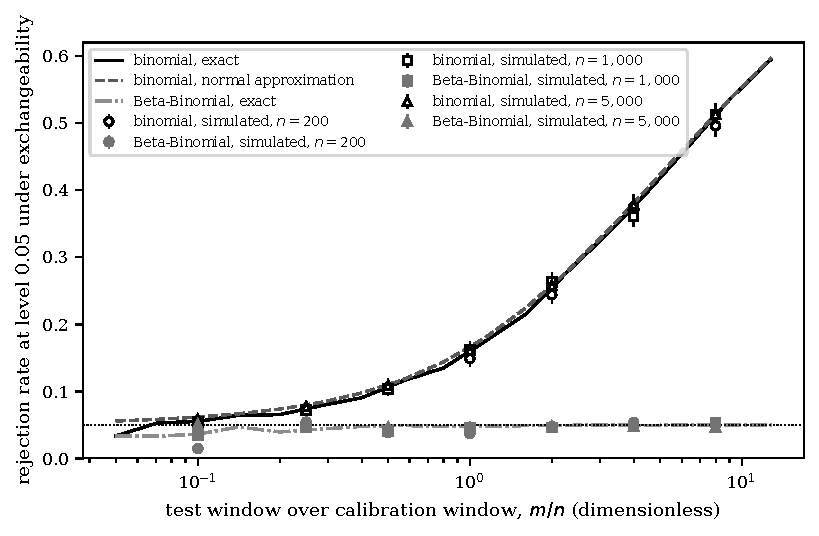
\includegraphics[width=0.92\textwidth]{coverage_size}
\caption{Rejection rate of the binomial and of the Beta-Binomial coverage test at the level 0.05 on exchangeable data, against the ratio of the test window to the calibration window; curves are the exact size and the normal approximation of the binomial test for 1,000 calibration rows, and points are the simulated rates for 200, 1,000 and 5,000 rows with two-standard-error bars over 4,000 replications.}
\label{fig:coverage-size}
\end{figure}

\paragraph{The rejection regions.} The size excess has a direct reading in terms of the coverage. At $n=m=1000$ the binomial test accepts an empirical coverage between \RegionBinLo{} and \RegionBinHi{}, and the Beta-Binomial test between \RegionBBLo{} and \RegionBBHi{}: the exact law of the count is wider than the binomial law, and the corrected test accepts a band of coverages that the binomial test would call a failure. \Cref{fig:rejection-regions} draws the two p-values as functions of the coverage, with the level 0.05 as a horizontal line; the binomial p-value falls below the level on the shoulders of the Beta-Binomial one.

\begin{figure}[htbp]
\centering
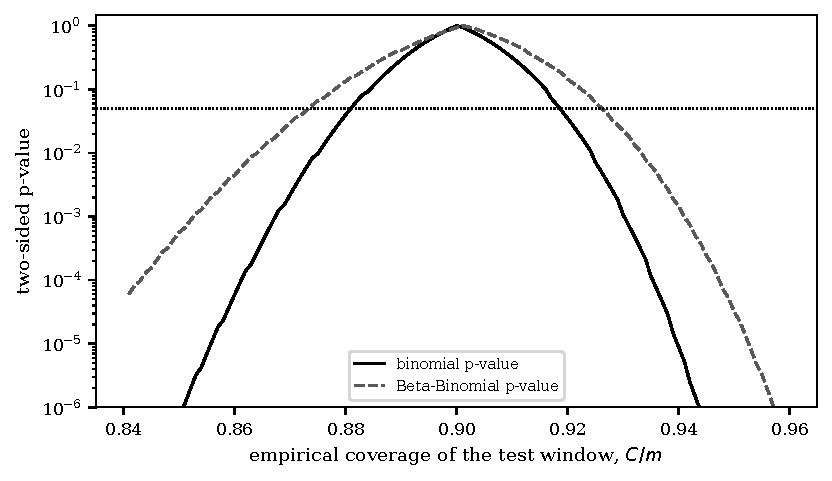
\includegraphics[width=0.92\textwidth]{rejection_regions}
\caption{The binomial and the Beta-Binomial two-sided p-value of a covered count as a function of the empirical coverage of a test window of 1,000 rows against a calibration window of 1,000 rows and the target 0.90, on a logarithmic axis, with the level 0.05 as the dotted line; the Beta-Binomial p-value stays above the level over a wider range of coverages.}
\label{fig:rejection-regions}
\end{figure}

\paragraph{Power.} With a drift of the test scores of shape $b=1.10$ the binomial test rejects in \CovPowBinBTen{} of the replications at equal windows and \CovPowBinCTen{} at four times the calibration window, against \CovPowBBBTen{} and \CovPowBBCTen{} for the Beta-Binomial test. The correction looks like a loss of power by that comparison, and \cref{fig:coverage-power} shows why the comparison is not meaningful: when the power is plotted against the coverage lost, the binomial test starts at its size excess (\CovSinBinB{} and \CovSinBinC{} at no loss) and rises on a curve that lies above the Beta-Binomial one by about the size excess, and the binomial test with the cut calibrated to the exact size 0.05 lies on the Beta-Binomial curve. At $b=1.10$ the calibrated binomial test rejects in \CovPowOracleBTen{} and \CovPowOracleCTen{} of the replications at the two windows, within \ExPowGapMax{} (exact) of the Beta-Binomial test over every window pair and drift shape of the exact power curves, as \cref{conj:power} states. The power that the binomial test appears to have in excess of the Beta-Binomial test is its size.

\begin{figure}[htbp]
\centering
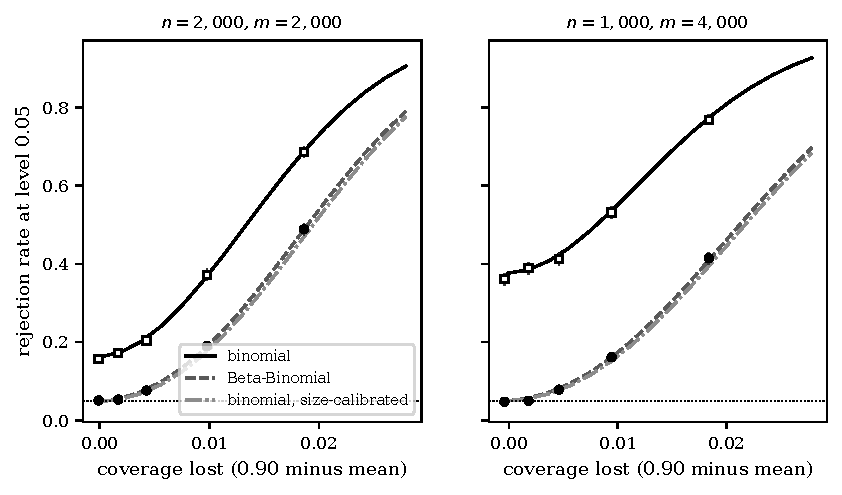
\includegraphics[width=\textwidth]{coverage_power}
\caption{Power of the binomial, the Beta-Binomial and the size-calibrated binomial coverage test against the coverage lost to the planted drift (0.90 minus the mean coverage), for equal windows of 2,000 rows (left) and for 1,000 calibration rows and 4,000 test rows (right); curves are exact, and points with two-standard-error bars are simulated over 4,000 replications.}
\label{fig:coverage-power}
\end{figure}

\subsection{The committed coverage evidence}

\Cref{tab:committed-conformal} lists the five conformal coverage rows of the committed shift variant of the credit model, with both p-values the engine returns, and \cref{fig:committed-p} draws the two p-values side by side on a logarithmic scale. The calibration window holds \CmNcal{} rows and each test window \CmBaseM{} rows (\CmPoolM{} for the pooled window), so the ratio $m/n$ is about 2.1, a ratio at which the binomial test has a size of about 0.25 (\cref{tab:exact-size}). At the baseline window, whose coverage is \CmBaseCov{}, both tests accept (p-values \CmBaseBB{} and \CmBaseBin{}) and the light is \CmBaseLight{}. At the windows shifted by 0.25 and by 0.5 times the size of the Federal Reserve higher-risk shift the coverage falls to \CmQuarterCov{} and \CmHalfCov{} and both p-values are far below $0.01$ (\CmQuarterBB{} and \CmHalfBB{} for the Beta-Binomial test), so the lights are \CmQuarterLight{} and \CmHalfLight{} whichever p-value is read; the pooled window is also \CmPoolLight{} (\CmPoolBB{}). The coverage is not monotone in the multiple of the shift (\CmQuarterCov{}, \CmHalfCov{} and then \CmOneCov{}); the three windows are the same holdout displaced by 0.25, 0.5 and 1 times one displacement of the leading features, and the committed document of the case reports the three values without a mechanism for the rise, which is not tested here. The window shifted by the full size has the coverage \CmOneCov{}, which is below the target by 0.02: the Beta-Binomial p-value is \CmOneBB{}, so the light is \CmOneLight{}, whereas the binomial p-value of the same count is \CmOneBin{}, below the red level 0.01, and a rule that read the binomial p-value would have set the light to red. This is the one window of five whose light the correction changes, and it changes it in the direction the size calculation predicts: after a calibration on \CmNcal{} rows, a coverage of \CmOneCov{} on \CmOneM{} rows is a count that the exact law of exchangeable data produces with a probability of \CmOneBB{} (the p-value), and that the binomial law, which ignores the randomness of the calibration quantile, calls \CmOneBin{} likely. Recomputing every committed p-value from its covered count with the engine function reproduces the committed value to \CmRecomputeDiff{} in the base-10 logarithm.

\begin{table}[htbp]
\centering
\small
\caption{The conformal coverage rows of the committed shift variant of the gradient-boosting model fitted on the Polish company bankruptcy data, evaluated on the locked holdout shifted by sizes taken from the Federal Reserve corporate portfolios: the calibration and test sizes, the empirical coverage against the target 0.90, both p-values of the engine and the light the Beta-Binomial p-value sets; the light never reads the binomial one.}
\label{tab:committed-conformal}
\fitwidth{\begin{tabular}{lrrcccl}
\toprule
Window & $n$ & $m$ & Coverage & $p$ Beta-Binomial & $p$ binomial & Light \\
\midrule
baseline & 1,471 & 3,151 & 0.8946 & 0.523 & 0.313 & green \\
higher risk x0.25 & 1,471 & 3,151 & 0.7509 & 2.13e-35 & 3.69e-127 & red \\
higher risk x0.5 & 1,471 & 3,151 & 0.7099 & 4.56e-52 & 1.19e-194 & red \\
higher risk x1 & 1,471 & 3,151 & 0.8800 & 0.0372 & 0.000258 & amber \\
pooled & 1,471 & 12,604 & 0.8089 & 2.86e-20 & 2.16e-207 & red \\
\bottomrule
\end{tabular}}
\end{table}


\begin{figure}[htbp]
\centering
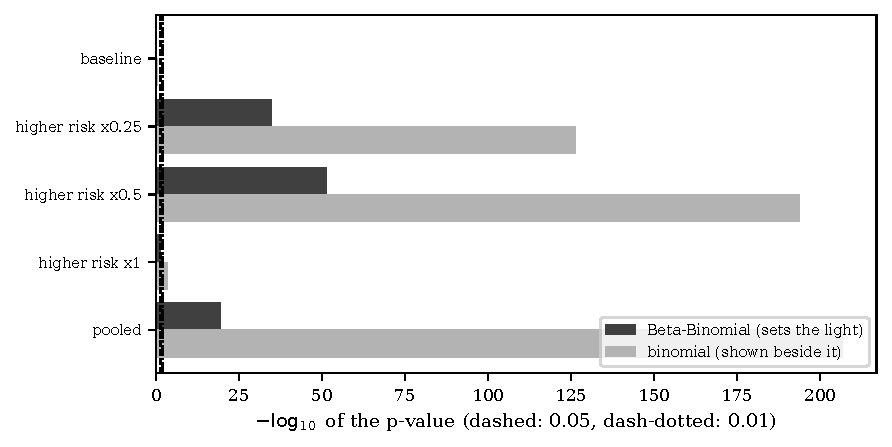
\includegraphics[width=0.92\textwidth]{committed_p}
\caption{Minus the base-10 logarithm of the Beta-Binomial and of the binomial p-value of each committed conformal coverage window of the credit-model shift case, with the levels 0.05 (dashed) and 0.01 (dash-dotted); bars longer than 8 are cut at 8, with their value printed. The two p-values set the same light on four windows; on the shifted and pooled windows both are far below 0.01 and differ by many orders of magnitude, and on the window of full Federal Reserve shift the binomial p-value (\CmOneBin{}) falls below 0.01 while the Beta-Binomial one (\CmOneBB{}) does not.}
\label{fig:committed-p}
\end{figure}

\subsection{The resilience test}

\paragraph{The null drop.} Without shift the AUC drop on the worst quarter is not centred on zero. At 500 evaluation rows its mean is \ShMeanDropCZ{}, its standard deviation \ShSdDropCZ{} and its 95th percentile \ShQNinetyFiveCZ{}, so a fixed cut of 0.05 is exceeded by \ShRateFixedFiveCZ{} of the null drops and a cut of 0.10 by \ShRateFixedTenCZ{}. \Cref{fig:shift-drops} shows the two histograms of the drops at shift 0 and shift 2. The mean of the drops that the permutation reference draws is \ShNullMeanCZ{}, close to the mean \ShMeanDropCZ{} of the observed null drops, which is what an exchangeable reference should give; the p-value reads the observed drop against the upper tail of the reference, and the rates below put its upper tail within about two standard errors of the exact grid size.

\begin{figure}[htbp]
\centering
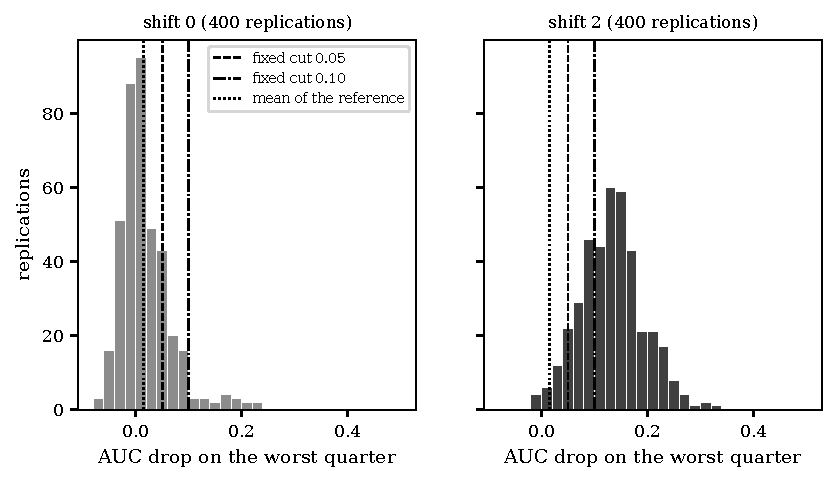
\includegraphics[width=\textwidth]{shift_drops}
\caption{Histograms of the AUC drop on the worst quarter of 500 evaluation rows over 400 replications without shift (left) and with a planted shift of two standard deviations (right), with the fixed cuts 0.05 and 0.10 and the mean of the null drops of the permutation reference as vertical lines.}
\label{fig:shift-drops}
\end{figure}

\paragraph{Size and power at 500 rows.} The fixed cut 0.05 raises a false alarm in \ShRateFixedFiveCZ{} of the shift-free replications (standard error \ShSeFixedFiveCZ{}) and the fixed cut 0.10 in \ShRateFixedTenCZ{} (\ShSeFixedTenCZ{}); the z rule gives \ShRateZruleCZ{} (\ShSeZruleCZ{}) and the permutation reference with 199 draws \ShRatePermCZ{} (\ShSePermCZ{}). At the planted shift of two standard deviations the four rules reject in \ShRateFixedFiveCT{}, \ShRateFixedTenCT{}, \ShRateZruleCT{} and \ShRatePermCT{} of the replications. The permutation reference therefore detects a planted shift less often than the fixed cut 0.05 in every cell with a shift, by at least \ShPermPowerGapMin{}, and the larger part of the difference is the false alarms of the cut. A fixed cut set at the 95th percentile of the null drops of the same cell, \ShOracleCut{} at 500 rows, has by construction the size \ShOracleRateZ{} and the power \ShOracleRateT{} at shift 2. Of the difference \ShFixedPermDiffT{} in power between the fixed cut 0.05 and the reference at shift 2, the calibrated cut also gives up \ShFixedOracleDiffT{}, and the reference gives up a further \ShOracleDiffT{}, at a standard error of \ShOracleDiffSe{}; the calibrated cut needs a simulation of the null that a validation team does not have.

\paragraph{The size of a fixed cut depends on the evaluation sample.} \Cref{tab:shift-eval-size} and \cref{fig:shift-eval-size} give the four rules at the four evaluation sizes. The fixed cut 0.05 raises a false alarm in \ShRateFixedFiveAZ{}, \ShRateFixedFiveBZ{}, \ShRateFixedFiveCZ{} and \ShRateFixedFiveDZ{} of the replications at 125, 250, 500 and 1,000 rows, and the cut 0.10 in \ShRateFixedTenAZ{}, \ShRateFixedTenBZ{}, \ShRateFixedTenCZ{} and \ShRateFixedTenDZ{}: the size falls as the evaluation sample grows, because the spread of the null drop falls, and the cut that would have size 0.05 (the 95th percentile of the null drops) is \ShQNinetyFiveAZ{}, \ShQNinetyFiveBZ{}, \ShQNinetyFiveCZ{} and \ShQNinetyFiveDZ{}. The cut 0.10 is close to calibrated at 500 rows and oversized at 125 rows, and a team that tuned it at 500 rows would carry a size of \ShRateFixedTenAZ{} to the smaller design. The permutation reference with 199 draws stays between \ShRatePermAZ{} and \ShRatePermCZ{} at every size, and the z rule between \ShRateZruleBZ{} and \ShRateZruleCZ{}.

The power of the permutation reference at shift 2 is \ShRatePermAT{}, \ShRatePermBT{}, \ShRatePermCT{} and \ShRatePermDT{} over the four sizes and the power of the fixed cut 0.05 is \ShRateFixedFiveAT{}, \ShRateFixedFiveBT{}, \ShRateFixedFiveCT{} and \ShRateFixedFiveDT{}; the difference is \ShPowGapAT{}, \ShPowGapBT{}, \ShPowGapCT{} and \ShPowGapDT{}, so it narrows as the evaluation sample grows. The z rule has less power than the reference at 125 and 250 rows (\ShRateZruleAT{} and \ShRateZruleBT{} against \ShRatePermAT{} and \ShRatePermBT{}) and more at 500 and 1,000 rows (\ShRateZruleCT{} and \ShRateZruleDT{} against \ShRatePermCT{} and \ShRatePermDT{}).

\begin{table}[htbp]
\centering
\small
\caption{The size (shift 0) and the power (shift 2) of four rules of the resilience test as the evaluation sample grows from 125 to 1,000 rows, with the development sample twice as large; rates with their standard errors over the replications of each cell.}
\label{tab:shift-eval-size}
\fitwidth{\begin{tabular}{llcccc}
\toprule
Rule & Rate & $n_{\mathrm{eval}}=125$ & 250 & 500 & 1,000 \\
\midrule
fixed 0.05 & size & $0.254 \pm 0.022$ & $0.212 \pm 0.020$ & $0.175 \pm 0.019$ & $0.125 \pm 0.017$ \\
fixed 0.05 & power & $0.709 \pm 0.023$ & $0.853 \pm 0.018$ & $0.925 \pm 0.013$ & $0.993 \pm 0.004$ \\
fixed 0.10 & size & $0.098 \pm 0.015$ & $0.068 \pm 0.013$ & $0.048 \pm 0.011$ & $0.040 \pm 0.010$ \\
fixed 0.10 & power & $0.520 \pm 0.025$ & $0.635 \pm 0.024$ & $0.703 \pm 0.023$ & $0.792 \pm 0.020$ \\
z rule & size & $0.035 \pm 0.009$ & $0.030 \pm 0.009$ & $0.065 \pm 0.012$ & $0.045 \pm 0.010$ \\
z rule & power & $0.188 \pm 0.020$ & $0.422 \pm 0.025$ & $0.723 \pm 0.022$ & $0.940 \pm 0.012$ \\
permutation, 199 & size & $0.048 \pm 0.011$ & $0.055 \pm 0.011$ & $0.062 \pm 0.012$ & $0.052 \pm 0.011$ \\
permutation, 199 & power & $0.317 \pm 0.023$ & $0.527 \pm 0.025$ & $0.680 \pm 0.023$ & $0.870 \pm 0.017$ \\
\bottomrule
\end{tabular}}
\end{table}


\begin{figure}[htbp]
\centering
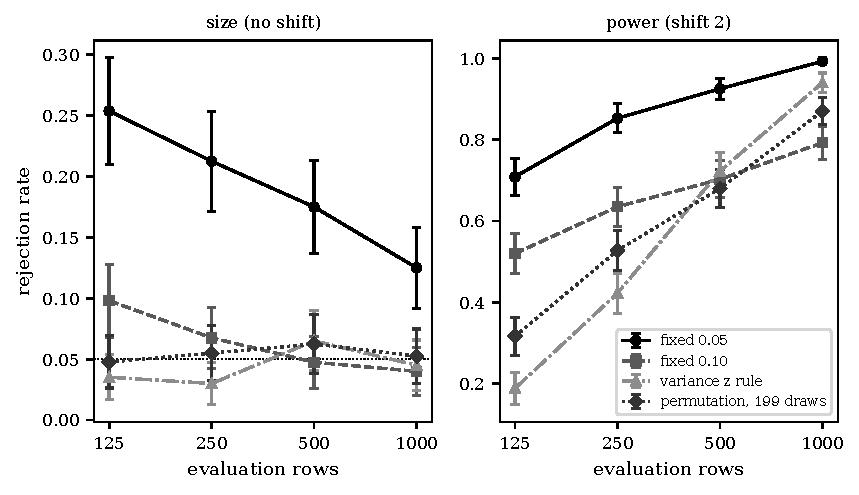
\includegraphics[width=\textwidth]{shift_eval_size}
\caption{Size at shift 0 (left) and power at a planted shift of two standard deviations (right) of four rules of the resilience test, the fixed cuts 0.05 and 0.10, the variance z rule and the permutation reference with 199 draws, against the number of evaluation rows, with two-standard-error bars over 400 replications per cell.}
\label{fig:shift-eval-size}
\end{figure}

\paragraph{The number of draws.} The permutation reference with 19 draws never rejects: the smallest attainable p-value is \GranSmallestNineteen{}, which is not below $0.05$, and the measured rate is \ShRatePermNineteenCZ{} at every size and shift. With 39, 99 and 199 draws the pooled sizes over the four evaluation sizes are \ShPermPooledThirtyNine{}, \ShPermPooledNinetyNine{} and \ShPermPooledFull{}, with standard errors of about \ShPermPooledSeFull{}, against the exact sizes \GranExactThirtyNine{}, \GranExactNinetyNine{} and \GranExactFull{} that \cref{prop:permutation} gives for an exchangeable reference; the measured sizes lie above the exact ones by \ShPermExcessThirtyNine{}, \ShPermExcessNinetyNine{} and \ShPermExcessFull{}, which is \ShPermExcessZMin{} to \ShPermExcessZMax{} of the measured standard errors and \ShPermExcessZExactMin{} to \ShPermExcessZExactMax{} of the standard error of the exact null rate. The three readings are not three observations: the references with 39 and 99 draws are the first draws of the 199 of the same replications, so they share replications and draws, and the common sign is one observation. At 500 rows the size is \ShRatePermCZ{} (\ShSePermCZ{}), within the bound of 0.05 plus two standard errors but above the exact 0.045 that an exchangeable reference gives. A possible cause, not tested here, is the approximate exchangeability of the engine's construction (a pseudo-development set of $n_d-n_e$ rows); no experiment varies the size of that set. The power rises with the number of draws, from \ShRatePermThirtyNineCT{} with 39 to \ShRatePermNinetyNineCT{} with 99 and \ShRatePermCT{} with 199 at 500 rows and shift 2 (\cref{fig:shift-draws}). The red light of the engine needs a p-value below $0.01$, which a reference with fewer than \RedMinDraws{} draws cannot give.

\begin{figure}[htbp]
\centering
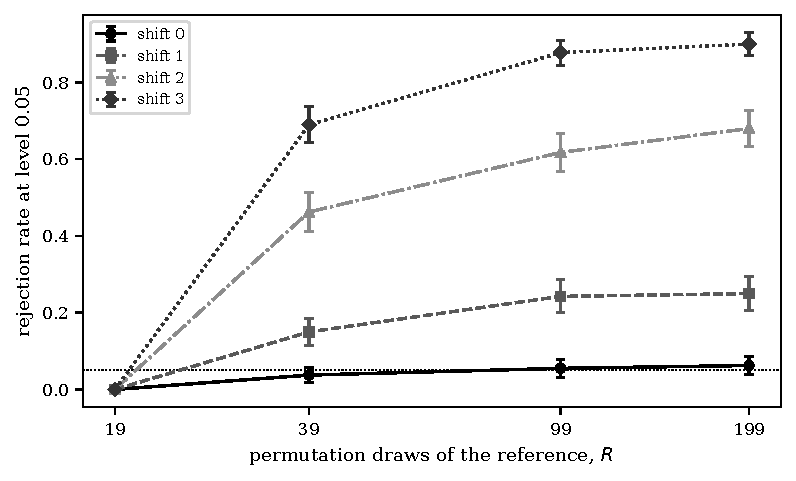
\includegraphics[width=0.85\textwidth]{shift_draws}
\caption{Rejection rate of the permutation reference at the level 0.05 as a function of its number of draws, at 500 evaluation rows and planted shifts of 0, 1, 2 and 3 standard deviations, with two-standard-error bars over 400 replications; the dotted line is the level 0.05.}
\label{fig:shift-draws}
\end{figure}

\paragraph{The committed resilience row.} The committed resilience row of the credit-model shift case has \CmResN{} evaluation rows, a worst share of 0.10 and the observed drop \CmResDrop{}. The \CmResDraws{} draws of the reference have a mean of \CmResNullMean{} and a 95th percentile of \CmResNullP{}, and none of them reaches the observed drop, so the p-value is the smallest the reference can give, \CmResP{}, and the light is red. A fixed cut of 0.05 would also have fired; the reference differs in that it says how far the drop is from what a shift-free sample of the same size gives.

\subsection{The situation-testing light}

\paragraph{The null law of the share.} With 400 applicants on the threshold-bias plant the protected group has about \SiComplainantsSmallZ{} complainants, the share of significant complainants has a mean of \SiMeanShareSmallZ{} and a standard deviation of \SiSdShareSmallZ{} without bias, and the design effect of \cref{eq:design-effect} is \SiDesignSmallZ{}; with 1,000 applicants the complainants number \SiComplainantsLargeZ{}, the mean share is \SiMeanShareLargeZ{}, the standard deviation \SiSdShareLargeZ{} and the design effect \SiDesignLargeZ{}. Independent complainants at the level 0.05 would give a standard deviation of \SiIndepSd{} at 200 complainants. \Cref{fig:situation-null-share} shows the two null histograms with the cuts 0.10 and 0.20: the distribution is right-skewed, with a tail that reaches above 0.10 at 400 applicants and almost not at 1,000.

\begin{figure}[htbp]
\centering
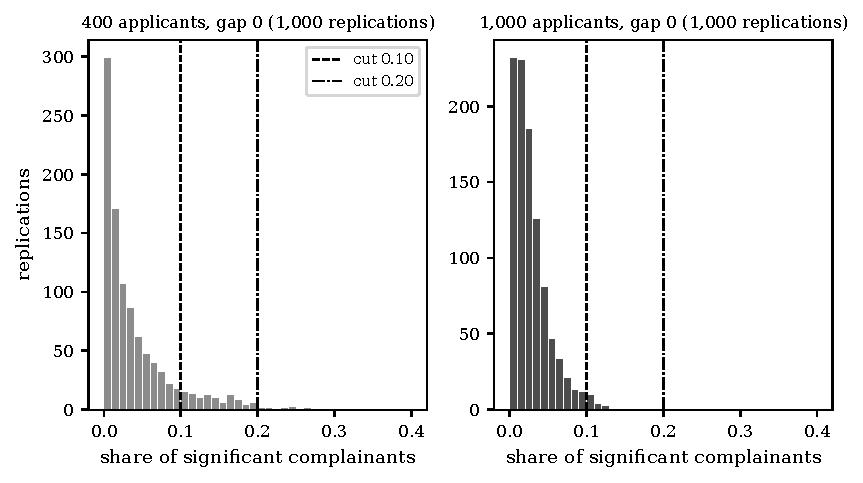
\includegraphics[width=\textwidth]{situation_null_share}
\caption{Histograms of the share of significant complainants without bias for 400 applicants over 1,000 replications (left) and 1,000 applicants over 1,000 replications (right), on the threshold-bias plant, with the amber cuts 0.10 and 0.20 as vertical lines; the right tail beyond 0.10 shrinks sharply as the number of applicants grows.}
\label{fig:situation-null-share}
\end{figure}

\paragraph{Size and power of the cuts.} With 400 applicants the cut 0.10 fires in \SiRateCutTenSmallZ{} of the null replications (standard error \SiSeCutTenSmallZ{}) and the cut 0.20 in \SiRateCutTwentySmallZ{} (\SiSeCutTwentySmallZ{}). At the planted gap 0.4 they detect the bias in \SiRateCutTenSmallC{} and \SiRateCutTwentySmallC{} of the replications and at the gap 0.8 in every replication. At the small gaps the cut 0.20 has less power: \SiRateCutTwentySmallB{} against \SiRateCutTenSmallB{} at the gap 0.2, and \SiRateCutTwentySmallA{} against \SiRateCutTenSmallA{} at the gap 0.1 (\cref{tab:situation-ablation}). With 1,000 applicants the cut 0.10 fires in \SiRateCutTenLargeZ{} of the null replications and the cut 0.20 in \SiRateCutTwentyLargeZ{}; the cut 0.20 detects the gap 0.2 in \SiRateCutTwentyLargeB{} of the replications. \Cref{fig:situation-cuts} shows the rates of the seven cuts at each gap: the curves of the null and of the planted gaps cross, so that every cut is a choice of a point on a trade between size and power that depends on the number of applicants.

\begin{figure}[htbp]
\centering
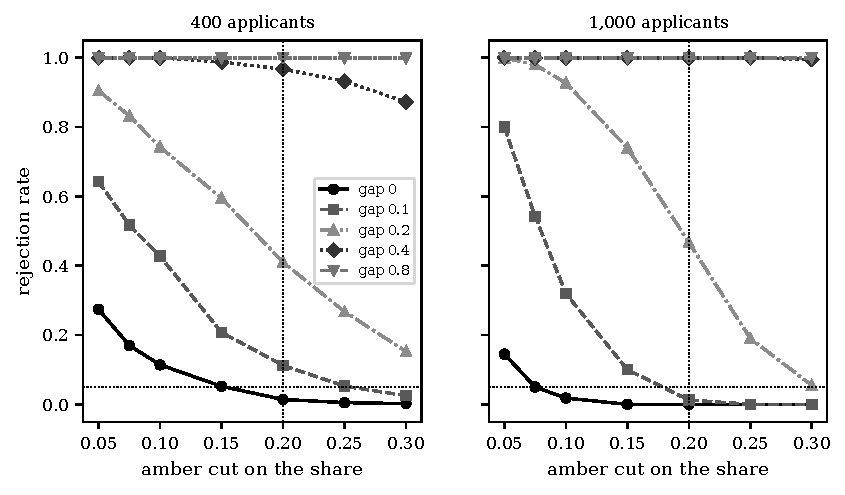
\includegraphics[width=\textwidth]{situation_cuts}
\caption{Rejection rate of the share cut as a function of the cut for 400 applicants (left) and 1,000 applicants (right) and the planted gaps 0, 0.1, 0.2, 0.4 and 0.8, over 1,000 replications at gap 0 and 400 at the others; the vertical dotted line is the engine's cut 0.20 and the horizontal dotted line the level 0.05.}
\label{fig:situation-cuts}
\end{figure}

\paragraph{A second data-generating process.} On the design of the engine's own size-and-power suite, with attributes that are independent of the decision, the null law of the share is different (\cref{tab:situation-designs}). At 400 applicants the cut 0.10 fires in \SiInRateCutTenSmallZ{} of the null replications (\SiInSeCutTenSmallZ{}) and the cut 0.20 in \SiInRateCutTwentySmallZ{} (\SiInSeCutTwentySmallZ{}), against \SiRateCutTenSmallZ{} and \SiRateCutTwentySmallZ{} on the threshold-bias plant. The engine's suite records a size of \EngSiSizeTwenty{} (standard error \EngSiSeTwenty{}) for the cut 0.20 and \EngSiSizeTen{} for the former cut 0.10 at 400 applicants and 30 neighbours on that design, and the values measured here, \SiInRateCutTwentySmallZ{} and \SiInRateCutTenSmallZ{}, reproduce them. At 1,000 applicants the sizes on the second design are \SiInRateCutTenLargeZ{} and \SiInRateCutTwentyLargeZ{}. The two designs differ in the size of the same cut by a factor of about two at 400 applicants, and the size of a cut at one number of applicants does not carry to another on either design. The cut chosen by \cref{eq:cut-rule} on the grid of the experiments is therefore \SiChosenThrSmall{} on the threshold-bias plant at 400 applicants (size \SiRateCutFifteenSmallZ{}, standard error \SiSeCutFifteenSmallZ{}) and \SiChosenIndSmall{} on the second design, where the cut 0.15 has size \SiInRateCutFifteenSmallZ{}.

\begin{table}[htbp]
\centering
\small
\caption{The null law of the share of significant complainants and the size of the amber cuts 0.10 and 0.20 on two planted designs without bias, for 400 and for 1,000 applicants: the mean number of complainants, the mean and standard deviation of the share, the variance of the count over the binomial variance, and the size with its Monte Carlo standard error over 1,000 and 2,000 replications.}
\label{tab:situation-designs}
\fitwidth{\begin{tabular}{llrrrrcc}
\toprule
Design & Applicants & Complainants & Mean share & SD of share & Design effect & Size, cut 0.10 & Size, cut 0.20 \\
\midrule
threshold-bias plant & 400 & 200 & 0.041 & 0.050 & 10.6 & $0.114 \pm 0.010$ & $0.014 \pm 0.004$ \\
threshold-bias plant & 1,000 & 500 & 0.028 & 0.023 & 5.8 & $0.018 \pm 0.004$ & $0 \text{ of } 1{,}000\ (<0.0030)$ \\
independent attributes & 400 & 160 & 0.055 & 0.062 & 12.8 & $0.195 \pm 0.009$ & $0.035 \pm 0.004$ \\
independent attributes & 1,000 & 400 & 0.055 & 0.038 & 12.3 & $0.128 \pm 0.007$ & $0.0005 \pm 0.0005$ \\
\bottomrule
\end{tabular}}
\end{table}


\paragraph{The other rules.} The one-sided binomial test of the count, which treats the complainants as independent, has size \SiRateCountBinSmallZ{} at 400 applicants on the threshold-bias plant and \SiInRateCountBinSmallZ{} on the second design, three to five times the level; the rule that rejects when one complainant is significant at the Bonferroni level has size \SiRateBonfSmallZ{} and \SiInRateBonfSmallZ{} and detects the gap 0.2 in \SiRateBonfSmallB{} of the replications, close to the share cut 0.20 (\SiRateCutTwentySmallB{}, within the error) and less than the share cut 0.10 (\SiRateCutTenSmallB{}).

\subsection{The committed fairness evidence}

\Cref{tab:committed-fair} lists the situation-testing row of each of the six committed year pairs of the mortgage decisions of Delaware. The number of complainants is between \CmFairQMin{} and \CmFairQMax{}, an order of magnitude or more above the \SiComplainantsSmallZ{} and \SiComplainantsLargeZ{} of the plants, and the shares of significant complainants are between \CmFairMin{} and \CmFairMax{}. With the amber cut 0.20, \CmFairAmber{} pairs are amber and \CmFairGreen{} are green; with the former cut 0.10 all \CmFairAboveTen{} pairs, whose share exceeds it, would be amber. The two green pairs have shares of \CmFairGreenLo{} and \CmFairGreenHi{}, just below the cut. The cut 0.20 was measured at 400 applicants, and the null share narrows as the complainants become more numerous (\cref{tab:situation-designs}), so at the committed size a null share at 0.20 is rarer than the measured size suggests; how much rarer is not measured here. The size of neither cut is measured at the committed number of complainants, so the two green pairs are not shown to be a gain: the null mean share of the plants is at most \SiNullMeanMax{}, and the green pairs have shares at least \CmFairGreenOverNull{} times that value. The cut 0.10 has the higher power at small gaps (\cref{tab:situation-ablation}), and at 1,000 applicants on the threshold-bias plant its size is \SiRateCutTenLargeZ{}, below the level, so setting the two pairs green may cost sensitivity and is not shown to improve the light.

\begin{table}[htbp]
\centering
\small
\caption{The situation-testing row of each committed Delaware mortgage year pair: the complainants of the protected group, how many are significant at level 0.05 with thirty neighbours, their share, the amber cut point the engine applies and the light that follows; the light is never red.}
\label{tab:committed-fair}
\fitwidth{\begin{tabular}{lrrccl}
\toprule
Year pair & Complainants & Significant & Share & Amber cut & Light \\
\midrule
2018-19 & 4,485 & 1,179 & 0.2629 & 0.20 & amber \\
2019-20 & 4,655 & 1,123 & 0.2412 & 0.20 & amber \\
2020-21 & 5,644 & 1,056 & 0.1871 & 0.20 & green \\
2021-22 & 8,113 & 1,616 & 0.1992 & 0.20 & green \\
2022-23 & 6,421 & 1,442 & 0.2246 & 0.20 & amber \\
2023-24 & 4,919 & 1,199 & 0.2437 & 0.20 & amber \\
\bottomrule
\end{tabular}}
\end{table}


\subsection{The predictions}

\Cref{tab:hypotheses} gives the outcome of each prediction. \HypHeld{} of the \HypTotal{} held: the binomial test rejects far above the level at equal windows and at four times the calibration window (H1a), the Beta-Binomial test stays within the bound of the level on the whole grid (H1b), the fixed cut 0.05 fires above the level without shift and the cut 0.10 at the smallest design (H2a), the reference stays within the bound of the level (H2b) and detects less than the fixed cut, by a margin that narrows with the sample (H2c), the cut 0.20 holds the level at 400 applicants and the cut 0.10 does not (H3a), and the cut 0.20 detects the largest planted gap (H3b). Of the rest, \HypRefuted{} were refuted. The cut 0.20 does lose power against the cut 0.10 at the small gaps (H3c): \SiRateCutTwentySmallB{} against \SiRateCutTenSmallB{} at the gap 0.2. The size of the cut 0.10 measured at 400 applicants does not carry to 1,000 applicants (H3d): \SiRateCutTenSmallZ{} at 400 and \SiRateCutTenLargeZ{} at 1,000. And the sizes are not the same on a second design (H3e): \SiRateCutTenSmallZ{} and \SiInRateCutTenSmallZ{} for the cut 0.10, \SiRateCutTwentySmallZ{} and \SiInRateCutTwentySmallZ{} for the cut 0.20. \HypPartial{} are held in part. The refuted ones all concern the situation light, which says that the corrections of the two other tests are on firmer ground than the cut of the third.


\section{Ablation}
\label{sec:ablation}
Each correction has components, and the ablation removes or changes them one at a time on the same replications, so that the contribution of each is a difference of paired rates. \Cref{tab:coverage-ablation}, \cref{tab:shift-ablation} and \cref{tab:situation-ablation} give the variants of the coverage test, the resilience test and the situation light.

\subsection{Components of the coverage test}

\begin{table}[htbp]
\centering
\small
\caption{The components of the coverage test removed or changed one at a time on the same covered counts: the size and the power at two shapes of drift for equal windows (the first three columns) and for a test window four times the calibration window (the last three); simulated rates with their standard errors.}
\label{tab:coverage-ablation}
\fitwidth{\begin{tabular}{p{5.2cm}cccccc}
\toprule
Variant & Size & Power, $b=1.05$ & Power, $b=1.10$ & Size  & Power, $b=1.05$  & Power, $b=1.10$  \\
\midrule
binomial p-value (published practice) & $0.157 \pm 0.006$ & $0.204 \pm 0.006$ & $0.372 \pm 0.008$ & $0.361 \pm 0.008$ & $0.412 \pm 0.008$ & $0.532 \pm 0.008$ \\
Beta-Binomial p-value, minimum-likelihood rule (proposed) & $0.051 \pm 0.003$ & $0.076 \pm 0.004$ & $0.190 \pm 0.006$ & $0.048 \pm 0.003$ & $0.079 \pm 0.004$ & $0.162 \pm 0.006$ \\
Beta-Binomial, equal-tail p-value & $0.052 \pm 0.004$ & $0.069 \pm 0.004$ & $0.179 \pm 0.006$ & $0.046 \pm 0.003$ & $0.070 \pm 0.004$ & $0.146 \pm 0.006$ \\
normal test with the variance ratio of Proposition 2 & $0.051 \pm 0.003$ & $0.076 \pm 0.004$ & $0.190 \pm 0.006$ & $0.047 \pm 0.003$ & $0.079 \pm 0.004$ & $0.162 \pm 0.006$ \\
Beta-Binomial with the calibration size halved & $0.018 \pm 0.002$ & $0.033 \pm 0.003$ & $0.102 \pm 0.005$ & $0.007 \pm 0.001$ & $0.020 \pm 0.002$ & $0.055 \pm 0.004$ \\
Beta-Binomial with the calibration size doubled & $0.089 \pm 0.005$ & $0.122 \pm 0.005$ & $0.264 \pm 0.007$ & $0.124 \pm 0.005$ & $0.164 \pm 0.006$ & $0.286 \pm 0.007$ \\
binomial with the exact size-calibrated cut & $0.052 \pm 0.004$ & $0.069 \pm 0.004$ & $0.179 \pm 0.006$ & $0.048 \pm 0.003$ & $0.072 \pm 0.004$ & $0.151 \pm 0.006$ \\
\bottomrule
\end{tabular}}
\end{table}


The first component is the law. Replacing the binomial law by the Beta-Binomial law lowers the size from \CovSinBinB{} to \CovSinBBB{} at equal windows and from \CovSinBinC{} to \CovSinBBC{} at four times the calibration window (\cref{tab:coverage-ablation}), and it lowers the power at the drift $b=1.10$ from \CovPowBinBTen{} to \CovPowBBBTen{} and from \CovPowBinCTen{} to \CovPowBBCTen{}. The second component is the rule that turns the law into a p-value. The equal-tail rule, which doubles the smaller tail, has the size \CovSinEqB{} and \CovSinEqC{} and the power \CovPowEqBTen{} and \CovPowEqCTen{} at $b=1.10$; the minimum-likelihood rule has a little more power (\CovPowBBBTen{} and \CovPowBBCTen{}), by a difference of about one to two standard errors, which does not separate the two rules. The third component is the exactness of the law. A normal test whose variance is the binomial variance times the factor of \cref{prop:variance} has the size \CovSinZinfB{} and \CovSinZinfC{} and the power \CovPowZinfBTen{} and \CovPowZinfCTen{}, indistinguishable from the exact law at these window sizes: the whole correction is carried by the variance factor, and the exact law matters for small windows, where the normal approximation of \cref{tab:exact-size} is off by as much as \CovNormalMaxErr{}.

The fourth component is the knowledge of the calibration size, which the law needs and the binomial test does not. A test that reads the law with half the true calibration size is conservative, with the size \CovSinHalfB{} and \CovSinHalfC{} and the power \CovPowHalfBTen{} and \CovPowHalfCTen{}; a test that reads it with double the size is oversized, \CovSinDoubleB{} and \CovSinDoubleC{}, though less than the binomial test at the same windows. An error of one rank in the quantile is nearly harmless: a test of rank $k$ applied to a calibration whose true rank is $k+1$ has the exact size \RankOffBBOne{} and \RankOffBBFour{} at the two windows, against \RankOffBinOne{} and \RankOffBinFour{} for the binomial test. The correction therefore needs the right calibration size, and the value of $n$ must be recorded with the conformal set, as the engine does; it does not need the rank to be right to the last unit. The fifth variant, the binomial test with its cut moved until the exact size is $0.05$, needs a p-value cut of \CovOracleCutB{} at equal windows and \CovOracleCutC{} at four times the calibration window instead of $0.05$; it has the size \CovSinOracleB{} and \CovSinOracleC{} and the power \CovPowOracleBTen{} and \CovPowOracleCTen{}, the power of the Beta-Binomial test within its error. A binomial test can be corrected by a cut that depends on $n$ and $m$, and the Beta-Binomial test gives the same behaviour without a cut that has to be computed for each pair $(n,m)$.

\subsection{Components of the resilience test}

\begin{table}[htbp]
\centering
\small
\caption{The rejection rate of each rule of the resilience test with 500 evaluation rows, 1,000 development rows and the worst quarter as the subsample: the size without shift and the power at three planted shifts, with the permutation reference read at four numbers of draws; rates with their standard errors.}
\label{tab:shift-ablation}
\fitwidth{\begin{tabular}{lcccc}
\toprule
Rule & Size (shift 0) & Power (shift 1) & Power (shift 2) & Power (shift 3) \\
\midrule
fixed drop above 0.05 & $0.175 \pm 0.019$ & $0.552 \pm 0.025$ & $0.925 \pm 0.013$ & $0.993 \pm 0.004$ \\
fixed drop above 0.10 & $0.048 \pm 0.011$ & $0.235 \pm 0.021$ & $0.703 \pm 0.023$ & $0.927 \pm 0.013$ \\
variance z rule & $0.065 \pm 0.012$ & $0.223 \pm 0.021$ & $0.723 \pm 0.022$ & $0.965 \pm 0.009$ \\
permutation reference, 19 draws & $0.000 \pm 0.000$ & $0.000 \pm 0.000$ & $0.000 \pm 0.000$ & $0.000 \pm 0.000$ \\
permutation reference, 39 draws & $0.037 \pm 0.009$ & $0.150 \pm 0.018$ & $0.463 \pm 0.025$ & $0.690 \pm 0.023$ \\
permutation reference, 99 draws & $0.055 \pm 0.011$ & $0.242 \pm 0.021$ & $0.618 \pm 0.024$ & $0.877 \pm 0.016$ \\
permutation reference, 199 draws & $0.062 \pm 0.012$ & $0.250 \pm 0.022$ & $0.680 \pm 0.023$ & $0.900 \pm 0.015$ \\
fixed drop above the 95th percentile of the null drops & $0.050 \pm 0.011$ & $0.242 \pm 0.021$ & $0.720 \pm 0.022$ & $0.927 \pm 0.013$ \\
\bottomrule
\end{tabular}}
\end{table}


\Cref{tab:shift-ablation} varies the rule at 500 evaluation rows. Standardising the drop with the variance of the structural components of the area, the z rule, brings the size from \ShRateFixedFiveCZ{} to \ShRateZruleCZ{} and keeps a power of \ShRateZruleCT{} at shift 2, close to the \ShRateFixedTenCT{} of the cut 0.10 and above the \ShRatePermCT{} of the reference. The reference does not use a closed-form variance; it measures the null law of the drop with the model, the selection of the worst subsample and the resemblance score all inside it, so it does not depend on the normal approximation of the area, which is the weaker the smaller the worst subsample. At 125 and 250 rows, where the worst quarter holds 32 and 63 rows, the reference has more power than the z rule (\cref{tab:shift-eval-size}), and at 500 and 1,000 rows less. The second component is the number of draws. With 39 draws the power at shift 2 is \ShRatePermThirtyNineCT{}, with 99 it is \ShRatePermNinetyNineCT{} and with 199 it is \ShRatePermCT{}, and the size rises from \ShRatePermThirtyNineCZ{} to \ShRatePermNinetyNineCZ{} and \ShRatePermCZ{} toward the level, as \cref{prop:permutation} predicts for a p-value grid that gets finer. The third component is the calibration of the cut by the null: the fixed cut at the 95th percentile of the null drops, the cut that needs a simulation the validation team does not have, has the size \ShOracleRateZ{} and the powers \ShOracleRateO{}, \ShOracleRateT{} and \ShOracleRateH{} at the shifts 1, 2 and 3, against \ShRatePermCO{}, \ShRatePermCT{} and \ShRatePermCH{} for the reference with 199 draws. The reference therefore reaches, within the error, the operating point of a cut that is calibrated on the null of the same cell, without the cell's null being simulated beforehand.

\subsection{Components of the situation-testing light}

\begin{table}[htbp]
\centering
\small
\caption{The rejection rate of nine rules of the situation-testing light: the size (gap 0) and the power at two planted gaps for 400 and for 1,000 applicants, with the standard error of every rate at most 0.025 over 1,000 replications at gap 0 and 400 at the others.}
\label{tab:situation-ablation}
\fitwidth{\begin{tabular}{lcccccc}
\toprule
Rule & $n=400$, gap 0 & gap 0.2 & gap 0.4 & $n=1{,}000$, gap 0 & gap 0.2 & gap 0.4 \\
\midrule
share cut 0.05 & 0.274 & 0.905 & 1.000 & 0.145 & 1.000 & 1.000 \\
share cut 0.075 & 0.170 & 0.833 & 1.000 & 0.050 & 0.980 & 1.000 \\
share cut 0.10 & 0.114 & 0.743 & 1.000 & 0.018 & 0.927 & 1.000 \\
share cut 0.15 & 0.052 & 0.595 & 0.988 & 0.000 & 0.740 & 1.000 \\
share cut 0.20 & 0.014 & 0.410 & 0.968 & 0.000 & 0.468 & 1.000 \\
share cut 0.25 & 0.005 & 0.268 & 0.932 & 0.000 & 0.190 & 1.000 \\
share cut 0.30 & 0.002 & 0.152 & 0.873 & 0.000 & 0.055 & 0.995 \\
binomial test of the count & 0.156 & 0.823 & 1.000 & 0.070 & 0.990 & 1.000 \\
one significant at the Bonferroni level & 0.079 & 0.453 & 0.938 & 0.053 & 0.760 & 1.000 \\
\bottomrule
\end{tabular}}
\end{table}


\Cref{tab:situation-ablation} varies the cut and the form of the rule. Moving the cut from 0.05 to 0.30 moves the size at 400 applicants from \SiRateCutFiveSmallZ{} to \SiRateCutThirtySmallZ{} and the power at the gap 0.2 from \SiRateCutFiveSmallB{} to \SiRateCutThirtySmallB{}; at 1,000 applicants the size is \SiRateCutFiveLargeZ{} at the cut 0.05 and zero from the cut 0.15, and the power at the gap 0.2 is \SiRateCutFiveLargeB{} and \SiRateCutThirtyLargeB{} at the two ends. The cut is the only parameter of the rule, so these are points on one operating curve, and the ablation of the cut is the curve. The binomial test of the count, which treats the complainants as independent, sits above the share cuts on that curve at 400 applicants: its size is \SiRateCountBinSmallZ{} and its power at the gap 0.2 is \SiRateCountBinSmallB{}, and the share cut 0.10 has the size \SiRateCutTenSmallZ{} and the power \SiRateCutTenSmallB{}, so that the binomial test buys its power with a size above the level, as the independence assumption predicts. The rule that fires when one complainant is significant at the Bonferroni level has the size \SiRateBonfSmallZ{} and the power \SiRateBonfSmallB{} at the same gap, and at 1,000 applicants the size \SiRateBonfLargeZ{} and the power \SiRateBonfLargeB{}. On this plant the share cuts dominate it: at 400 applicants the cut 0.15 has the smaller size (\SiRateCutFifteenSmallZ{}) and the larger power (\SiRateCutFifteenSmallB{}), and at 1,000 applicants the cut 0.10 has the size \SiRateCutTenLargeZ{} and the power \SiRateCutTenLargeB{}. The cut 0.20 is not on the efficient part of the curve at 1,000 applicants: its size is \SiRateCutTwentyLargeZ{}, like that of the cut 0.15, and its power at the gap 0.2 is \SiRateCutTwentyLargeB{} against \SiRateCutFifteenLargeB{}. The choice among these points is a choice of the error to avoid. The rule of \cref{eq:cut-rule} selects \SiChosenThrSmall{} on the threshold-bias plant at 400 applicants and \SiChosenThrLarge{} at 1,000, and \SiChosenIndSmall{} and \SiChosenIndLarge{} on the plant with independent attributes; the engine's cut of 0.20 is the choice of the second plant at 400 applicants, and it is conservative on the others.


\section{Discussion}
\label{sec:discussion}
The three corrections remove false alarms. They do so for three different reasons, and the reasons say how far each result extends.

\subsection{Why the rules behave as they do}

The binomial coverage test is oversized because it treats the nominal coverage as the coverage of the set. The coverage of a conformal set is a random variable that has the Beta law of \cref{prop:law}, and a test window that is long against the calibration window sees the fluctuation of that variable many times over: the variance of the count is the binomial variance times $(m+n+1)/(n+2)$ (\cref{prop:variance}), which is \VarRatioC{} at equal windows of 1,000 rows and \VarRatioD{} at a test window four times the calibration window. The size of the binomial test is therefore a function of the ratio $m/n$ and not of the calibration size alone, as \cref{fig:coverage-size} shows, and the exact size converges to the limit of \cref{prop:binomial-size}. The false alarms of the binomial test are not noise around a small error: at a ratio of 4 the test rejects more than a third of the exchangeable windows, and a validation team reading it on out-of-time windows that are longer than the calibration sample would conclude that most stable models have drifted.

The fixed AUC-drop cut is oversized at small evaluation samples for a different reason. The drop on the worst subsample has a positive mean and a standard deviation that falls with the evaluation sample (\cref{conj:scale}), so a fixed cut has a size that depends on the sample size: \ShRateFixedFiveAZ{} at 125 rows and \ShRateFixedFiveDZ{} at 1,000 rows for the cut 0.05, and the cut 0.10 changes from over-sized to nearly calibrated to slightly conservative over the same range. The permutation reference removes the dependence because its null law is drawn at the sample size of the evaluation set, and its size stays between \ShRatePermAZ{} and \ShRatePermCZ{}. The fixed cuts have more power, and the reason is size: a cut calibrated to the size 0.05 has the power of the reference to within the error.

The amber cut of the situation light is the least transferable of the three. The share of significant complainants has a null law that depends on the number of applicants and on the structure of the data (\cref{tab:situation-designs}), so the false-alarm rate of a cut is a property of a cut, a size of portfolio and a design of the data, and the proposition that bounds it from the mean alone is attained by laws that the data do not realise (\cref{prop:share}). The cut 0.20 has a size below the level on both plants at 400 and 1,000 applicants. That is a consequence of a conservative choice at 400 applicants and not a property of the cut: at 1,000 applicants on the threshold-bias plant the size is \SiRateCutTwentyLargeZ{} and the power at the gap 0.2 is \SiRateCutTwentyLargeB{}, against \SiRateCutTenLargeB{} for the cut 0.10 at the size \SiRateCutTenLargeZ{}.

\subsection{What the product should do}

Four practices follow from the measurements, and the corrected tests of the engine already follow the first three. The calibration size must be recorded with a conformal set, because the law needs it and a wrong value shifts the size (\cref{tab:coverage-ablation}); the engine stores \texttt{n\_cal} beside the covered count. The Beta-Binomial p-value sets the light and the binomial p-value is kept beside it, so that a reader who has used the binomial rule can see where the two differ; on the committed windows they differ in the light of one of five. The permutation reference needs at least \RedMinDraws{} draws to be able to set a red light, and the default 199 allows a p-value of 0.005. The fourth practice is not yet followed: the amber cut of the situation light is set from a measurement at one number of applicants and one design, and it should be re-measured, by \cref{eq:cut-rule}, on a plant that has the size and the neighbour structure of each portfolio to which the light is applied. At the committed sizes of \CmFairQMin{} to \CmFairQMax{} complainants, the null share is narrower than at 400 applicants, so the cut 0.20 is likely conservative there and the amber light is less sensitive than it could be at the same size; the measurement of that size is the next step.

\subsection{Negative and partial results}

Three of the predictions are refuted. The cut 0.20 loses power against the cut 0.10 at small gaps (H3c); the size measured at 400 applicants does not carry to 1,000 (H3d) or to a second design (H3e). The permutation reference has less power than the fixed cut 0.05 in every cell, by at least \ShPermPowerGapMin{}, and it has less than the z rule at 500 and 1,000 evaluation rows; its advantage is in the size at small samples and in the absence of a calibration, and not in power. The measured size of the permutation reference lies above the exact size of its p-value grid by about 0.01 at 39, 99 and 199 draws (\ShPermExcessZMin{} to \ShPermExcessZMax{} standard errors), so the reference is not exactly valid in the engine's construction, even if its size stays within the bound of the predictions. The Beta-Binomial correction does not lose power in the sense of \cref{conj:power}, but it is not powerful: at a coverage lost of 0.01 with equal windows of 2,000 rows it rejects \CovPowBBBTen{} of the replications at $b=1.10$, so a validation team that needs to detect a loss of 0.01 in coverage reliably needs longer windows.

\subsection{Position against the published methods}

The Beta law of the conditional coverage and the Beta-Binomial law of the empirical coverage on a validation window are published \citep{vovk2012,angelopoulos2021}, and the variance factor of \cref{prop:variance} is the published variance of that law. What the measurement adds is that the test a validation team would write from the binomial law, which is the natural one, has the sizes of \cref{tab:exact-size}, and that its apparent advantage in power is its size. The permutation reference is a Monte Carlo test with valid p-values \citep{phipson2010,davison1997}; what is added is its use on the worst-subsample drop of a resilience test \citep{sudjianto2023} with development rows as the null, and the measurement of what it costs. The situation-testing light uses the per-complainant test of Alvarez and Ruggieri \citep{alvarez2025} and adds nothing to it; the measurement concerns the portfolio-level share and its cut point. The corrections are ordinary statistical practice applied to a validation battery; the contribution is the measurement and the decision rules that it supports.


\section{Limitations}
\label{sec:limitations}
The results hold for the plants, the sample sizes and the parameters of the experiments, and the threats to their validity are of three kinds.

\subsection{Internal validity}

Every rate is a Monte Carlo estimate with a standard error of at most 0.025 (the resilience and situation rates near 0.5) and of about 0.003 to 0.008 for the coverage rates, so differences smaller than twice the standard error of the difference are not claimed. Several predictions are judged by comparing a rate with the level plus twice its standard error, a bound that has a false-rejection probability of about one in forty on each comparison; the manuscript reports the ranges over grids and names the cells where a difference is within the error, but it applies no correction for the number of comparisons. The coverage experiment evaluates the variants on the covered count, which is the only statistic that the tests read; the vectorised p-value tables are checked against the engine function on every replication (\CovEngineMismatches{} mismatches over \CovTotalReps{}), and against the exact sizes by summation, so the risk of a bug that the checks do not catch is small, though the resilience and situation experiments call the engine functions directly and have no second implementation to compare with. The permutation reference may not be exactly valid in the engine's construction: its pseudo-development set has fewer rows than the real development set, and the pooled sizes exceed the exact sizes of the p-value grid by about 0.01 (one observation, its cause not tested; \cref{sec:results}).

\subsection{External validity}

The generators are plants chosen to isolate one defect each, and a bank's data realise other nulls and other defects. The coverage test is the exception for its null, which is exact for every continuous score distribution; its power is measured for one family of drifts, in which the test scores are raised to a power, and a drift that moves the scores in a different way (a change in the dispersion, a change of the correlation between the score and the label) has a different power. Ties in the scores, which discrete scores produce, are outside \cref{prop:law}: a model with few distinct scores gives a set that covers more rows than the continuous law allows, and the Beta-Binomial test is then not exact. The windows are assumed exchangeable with the calibration rows under the null; a time series of out-of-time windows has autocorrelation, and the test is then oversized by an amount that the experiments do not measure. The resilience experiment fixes the development sample at twice the evaluation sample, the worst share at 0.25 (the committed run uses 0.10), one model and one shift direction. The situation experiments use 30 neighbours, one distance and two designs, and sizes of 400 and 1,000 applicants; the committed fairness evidence has \CmFairQMin{} to \CmFairQMax{} complainants, and the behaviour of the null share between 1,000 applicants and that size is not measured.

\subsection{Construct validity}

A rejection counts as a detection when the plant has a defect, and as a false alarm when it has none, and the defects are the ones the plants plant. The shift of the resilience plant is a shift in the covariates in a region where the true model changes, so that the model fails on the shifted rows by construction; a shift that does not change the model's ranking is not a defect, and the test is not designed to detect it. The bias of the situation plants is a lower cut-off or a higher probability of a negative decision for the protected group; a bias that acts only through attributes that the test matches on is not detected by a ceteris-paribus comparator, and the manuscript does not claim that it is. The size of the situation light is measured against the absence of a group effect, and the light reports no legal conclusion; a green light is not a finding of fairness and an amber light is not a finding of discrimination.

\subsection{Scope}

The manuscript does not claim that the Beta-Binomial law is new; it is published \citep{vovk2012,angelopoulos2021}. It does not claim that the permutation reference is optimal; it compares it with four other rules on one plant. It does not claim the cut 0.20 is the best cut for any portfolio; it shows that the size of a cut has to be measured on a plant that resembles the portfolio. The committed rows of the product are shown as the behaviour of the corrected rules on the product's data and not as a measurement of any error rate, because their truth is not planted. Conformal prediction under covariate shift and under online updating \citep{tibshirani2019,gibbs2021,barber2023} changes the null of the coverage test, and the tests of this manuscript do not apply to a set that is built for a shift. The sizes of the corrected rules are measured in the generators of the engine at the settings of the experiments, and a bank that applies the rules to its own data should repeat the measurement with a plant that has the sample sizes and the structure of that data, using the protocol of \cref{alg:protocol}.


\section{Reproducibility}
\label{sec:reproducibility}
The code, the committed results and the data are in the repository of the product, in the manuscript folder that holds this source. The experiments call the engine \texttt{riskvalidation} release \EnvEngine{} with \texttt{numpy} \EnvNumpy{} and \texttt{scipy} \EnvScipy{}; the engine is published on the Python Package Index and installs with \texttt{pip install riskvalidation}. The experiments need no external data. The repository and the inputs that the evidence reads are the following.
\begin{itemize}
\item The repository: \url{https://github.com/fsantibanezleal/CAOS_Contraste}.
\item The coverage evidence: \url{data/derived/C20/fed-shift.json}.
\item The fairness evidence: the six files \url{data/derived/C21/pair-*.json}.
\item The small-design figures of the predictions, read from the saved outputs of notebook 09 in the folder \url{notebooks/en/13-ml-and-ai-risk}.
\end{itemize}

Every table, figure and number rebuilds from the repository root with the commands below, in which \texttt{FOLDER} stands for the manuscript folder. The environment variable \texttt{CAOS\_TEMP\_ROOT} names a temporary folder for the per-cell caches, or each script takes \texttt{--cache}; the compact results that the manuscript reads are committed in the subfolder \texttt{experiments/results}.
\begin{verbatim}
python manuscripts/FOLDER/experiments/exact_theory.py
python manuscripts/FOLDER/experiments/exp_coverage.py
python manuscripts/FOLDER/experiments/exp_shift.py
python manuscripts/FOLDER/experiments/exp_situation.py
python manuscripts/FOLDER/experiments/exp_situation_indep.py
python manuscripts/FOLDER/make_tables.py
python manuscripts/FOLDER/make_numbers.py
python manuscripts/FOLDER/make_figures.py
python -m pytest manuscripts/FOLDER/experiments
\end{verbatim}
The root seed of every random stream is \RootSeed{}, and a replication has its own stream built from the experiment, the cell and the replication index, so the experiments are deterministic and independent of the number of worker processes. A second run from an empty cache reproduces the committed results of the first four experiments byte for byte. On 24 worker processes the resilience experiment, the longest, runs in about 14 minutes, and each of the others in under four minutes. The tests of the experiment scripts check the vectorised p-values against the engine function and against \texttt{scipy}, the exact sizes against their guarantees, the variance factor of \cref{prop:variance} against the summed law, and the seed reproducibility of a replication.


\section{Conclusions}
\label{sec:conclusions}
The three corrections of the validation battery remove most of the false alarms of the rules they replace, and each has a price that the measurement states. The coverage test of a split-conformal set, read against the Beta-Binomial law of the covered count, has an exact size that never exceeds \CovBBMaxExact{} on a grid of \CovGridCells{} window pairs, whereas the binomial test rejects \CovSinBinB{} of exchangeable windows at equal windows and \CovSinBinC{} at four times the calibration window. The power that the binomial test seems to gain is its size: a binomial test calibrated to the exact size has the power of the Beta-Binomial test within \ExPowGapMax{}. The resilience test, read against a permutation reference built from development rows, holds the level (\ShRatePermCZ{} at 500 evaluation rows against \ShRateFixedFiveCZ{} for a fixed drop of 0.05) and detects a planted shift of two standard deviations in \ShRatePermCT{} of the replications against \ShRateFixedFiveCT{}, a difference that narrows as the evaluation sample grows. The situation-testing light with the amber cut 0.20 holds the level at 400 applicants (\SiRateCutTwentySmallZ{} against \SiRateCutTenSmallZ{} for the cut 0.10) and detects a planted gap of 0.4 in \SiRateCutTwentySmallC{} of the replications, and it costs power at small gaps.

Of the \HypTotal{} predictions, \HypRefuted{} are refuted, and they bound the claim. The size of an amber cut is not a property of the cut: it depends on the number of applicants and on the data-generating process, and a cut measured on one plant is not transferable to another. The permutation reference has less power than the fixed cut it replaces in every cell. The Beta-Binomial law is published, so what this measurement contributes is the test that the law supports, its exact size and the measured error of the binomial test that a validation team would write.

The next steps follow from the limits. The coverage test should be measured on windows with serial dependence and on discrete scores, where its null is not exact. The resilience reference should be measured with a pseudo-development set of the size of the real development set, to remove the excess of the size over its exact value. The situation light needs its cut measured on plants with the size and the neighbour structure of each portfolio, in particular at the thousands of complainants of the committed evidence, where the null share is not measured here.


\bibliographystyle{plainnat}
\bibliography{references}

\end{document}
